% \documentclass[8pt,xcolor=pdftex,table,handout]{beamer}

\documentclass[8pt,xcolor=pdftex,table]{beamer}
\mode<presentation>

\usepackage[utf8]{inputenc}
\usepackage{lmodern}
\usepackage[T1]{fontenc}


% \usepackage{mathenv}
\usepackage{array}
% \usepackage{amsmath}
\usepackage{mathtools}% Loads amsmath
\usepackage{wasysym}
\usepackage{amsfonts}
\usepackage{amssymb, amsbsy}
\usepackage[utf8]{inputenc}
\usepackage{graphicx}
\usepackage{multimedia}
\usepackage{multicol}
\usepackage{multirow}
\usepackage{fourier}
\usepackage{makecell}


% \usepackage{colortbl}

% %\usepackage{textcomp}
% \usepackage{eurosym}

% % \usepackage{color}

% \usepackage{cancel}
% \usepackage{enumitem}

%\usepackage[active,tightpage]{preview}
% \usepackage{times}
\usepackage{tikz}
\usetikzlibrary{shapes,arrows,shadows,calc, angles}
\usetikzlibrary{arrows,shapes}
\usetikzlibrary{positioning}

\usepackage{verbatim}

\tikzstyle{format} = [draw, thin, fill=blue!20]
\tikzstyle{medium} = [ellipse, draw, thin, fill=green!20, minimum height=2.5em]


\tikzstyle{box_style0}=[draw, rounded corners ,
anchor=center,text centered,text=white, font=\bfseries] % text width=33mm,

\tikzstyle{box_style}=[box_style0, fill=black!80] % text width=33mm,

% \tikzstyle{bStyle}=[draw, rounded corners , fill=black!80,
% anchor=base, text centered,text=white, text width=2.8cm,font = 33]
\tikzstyle{bStyle2}=[draw, rounded corners , fill=black!80,
anchor=base,text centered,text=white, font=\bfseries] % text width=33mm,

\tikzstyle{bStyle0}=[draw, rounded corners , fill=b1,
anchor=base,text centered,text=white, font=\bfseries, align=center] % text width=33mm,
\tikzstyle{bStyle1}=[draw, rounded corners , fill=g1,
anchor=base,text centered,text=white, font=\bfseries] % text width=33mm,

\tikzstyle{bStyle3}=[draw, rounded corners , fill=r1,
anchor=base,text centered,text=white, font=\bfseries, align=center] % text width=33mm,

\tikzstyle{myarrow0}=[->, >=triangle 60, very thick, rounded corners=1mm]
\tikzstyle{myarrow}=[->, >=stealth, very thick, rounded corners=2mm]
\tikzstyle{line}=[thick]


% \usepackage[final]{movie15}
% \usepackage{media9}

%\setbeamertemplate{mini frame in other subsection}[default][0]

% \usepackage{ulem}

% \usepackage{stackengine}
\usepackage[cm]{sfmath}
\renewcommand\dot[1]{\text{\stackon[1pt]{$#1$}{.}}}

% \usepackage{siunitx}
% \sisetup{detect-all}   % ...this to force siunitx to actually use your fonts
% \usepackage{helvet}    % set the normal font here
% \usepackage{sansmath}  % load up the sansmath so that math -> helvet
% \sansmath               % <- tricky! -- gotta actually tell tex to use!


\beamertemplatenavigationsymbolsempty

\newcommand{\RightCrlBrc}[1]{$\pmb{\left. \rule{0pt}{#1}\right\}} $}

\newcommand{\TextSoulign}[3]{\textcolor{#1}{\underline{#2\textcolor{black}{#3}}}}
\newcommand\dgs[0]{$^\circ$}
\newcommand\dgsC[0]{$\,^{\circ}{\rm C}$}

\newcommand\up[1]{$^{\text{#1}}$}
\newcommand*\dif{\mathop{}\!\textnormal{\slshape d}}


\newcommand\tbf[1]{\textbf{#1}}
\newcommand\tit[1]{\textit{#1}}
\newcommand\tcit[2]{\textcolor{#1}{\textit{#2}}}

\newcommand{\chckmrk}[0]{\Large \textcolor{mygreen}{\checkmark}}

\definecolor{myOrng}{rgb}{0.9,0.5,0}
\renewcommand{\alert}[1]{\textcolor{myOrng}{\tbf{#1}}}




\PassOptionsToPackage{unicode}{hyperref}
\PassOptionsToPackage{naturalnames}{hyperref}

\usetheme[titleformat=smallcaps, subsectionpage=progressbar]{metropolis} % usetitleprogressbar, subsectionpage=progressbar
% default, professionalfonts, serif, structurebold, structureitalicserif, structuresmallcapsserif
% \usefonttheme{professionalfonts}

% \usetikzlibrary{calc,decorations.pathmorphing,decorations.pathreplacing}
% \usetikzlibrary{calc,trees,positioning,arrows,chains,shapes.geometric,%
%     decorations.pathreplacing,decorations.pathmorphing,shapes,%
%     matrix,shapes.symbols}
%     \usepackage{tikz-3dplot}
% \usetikzlibrary{patterns}


% \usetheme[compress]{Berlin}
\definecolor{g1}{rgb}{0,0.4,0}
\definecolor{b1}{rgb}{0,0,0.6}
\definecolor{r1}{rgb}{0.7,0,0}
\definecolor{k1}{rgb}{0.2,0.2,0.2}



\definecolor{myBckgrd}{rgb}{0,0,0}
\definecolor{myShaded}{rgb}{0.5,0.5,0.5}
\definecolor{myFnt}{rgb}{0.84,0.84,0.84}

\definecolor{clrBorders}{rgb}{0,0,0}
% \definecolor{clrBorders}{rgb}{1,1,1}

\definecolor{violetOC}{rgb}{0.455,0.318,0.922}

\definecolor{dfFirstRow}{rgb}{0.18,0.18,0.18}
\definecolor{dfEvenRow}{rgb}{0.118,0.118,0.118}
\definecolor{dfOddRow}{rgb}{0.149,0.149,0.149}




\definecolor{myCyan}{rgb}{0,0.8,0.99}
\definecolor{mygreen}{rgb}{0,0.35,0}
\definecolor{myGreen}{rgb}{0,0.8,0}
\definecolor{myred1}{rgb}{0.2,0,0}
\definecolor{myred2}{rgb}{0.4,0,0}
\definecolor{myred3}{rgb}{0.6,0,0}

% \setbeamercolor*{background}{c3}
% \setbeamercolor*{palette primary}{use=structure,fg=white,bg=myred3}
% \setbeamercolor*{palette secondary}{use=structure,fg=white,bg=myred2}
% \setbeamercolor*{palette tertiary}{use=structure,fg=white,bg=myred1}
% \setbeamercolor*{palette quaternary}{use=structure,fg=white,bg=myred1}
% \setbeamercolor{father}{fg=red}
% \setbeamercolor{mother}{fg=black}
% %\setbeamercolor{child}{parent={father,mother}}
% % \setbeamercolor{enumerate item}{parent=item} \setbeamercolor{enumerate subitem}{parent=subitem} \setbeamercolor{enumerate subsubitem}{parent=subsubitem}
% \setbeamercolor{item}{use={father,mother text},fg=father.fg!55!mother text.fg}





\setbeamercolor{button}{bg=myred3,fg=black}


% \author[Durand-Texte]{Thomas Durand-Texte - thomas.durand-texte@univ-lemans.fr}}


%\pgfdeclareimage[height=0,25cm]{logoCNAM}{/users/LABO/recherche/Completion/figures/Logo_cnam.jpg}
%\pgfdeclareimage[height=0,25cm]{logoCNAM}{Logo_cnam}
%\logo{\pgfuseimage{logoCNAM}}
\linespread{1.4}


% background image
% \pgfdeclareimage[height=96mm,width=128mm]{nombidon}{ploum}
% \setbeamertemplate{background}{\pgfuseimage{nombidon}}




\setbeamertemplate{footline}[frame number]



\makeatletter
\let\beamer@writeslidentry@miniframeson=\beamer@writeslidentry
\def\beamer@writeslidentry@miniframesoff{%
	\expandafter\beamer@ifempty\expandafter{\beamer@framestartpage}{}% does not happen normally
	{%else
		% removed \addtocontents commands
		\clearpage\beamer@notesactions%
	}
}
\newcommand*{\miniframeson}{\let\beamer@writeslidentry=\beamer@writeslidentry@miniframeson}
\newcommand*{\miniframesoff}{\let\beamer@writeslidentry=\beamer@writeslidentry@miniframesoff}
\makeatother

\defbeamertemplate*{headline}{miniframes theme no subsection}
{%
	\begin{beamercolorbox}[colsep=1.5pt]{upper separation line head}
	\end{beamercolorbox}
	% \begin{beamercolorbox}{section in head/foot}
	% 	\vskip2pt\insertnavigation{\paperwidth}\vskip2pt
	% \end{beamercolorbox}%
	% \begin{beamercolorbox}[colsep=1.5pt]{lower separation line head}
	% \end{beamercolorbox}
}

\setbeamertemplate{footline}[miniframes theme no subsection]

\setbeamerfont{subsubsection in toc}{size=\normalsize}
\setbeamercolor{section in toc}{fg=black}
\setbeamercolor{subsection in toc}{fg=black}

\makeatletter
\setbeamertemplate{footline}{%
	\begin{beamercolorbox}[colsep=1.5pt]{upper separation line foot}
	\end{beamercolorbox}
	% \begin{beamercolorbox}[ht=2.5ex,dp=1.125ex,%
	% 	leftskip=.3cm,rightskip=.3cm plus1fil]{author in head/foot}%
	% 	\leavevmode{\usebeamerfont{author in head/foot}\insertshortauthor}%
	% 	\hfill%
	% 	{\usebeamerfont{institute in head/foot}\usebeamercolor[fg]{institute in head/foot}\insertshortinstitute}%
	% \end{beamercolorbox}%
	\begin{beamercolorbox}[ht=2.5ex,dp=1.125ex,%
		leftskip=.3cm,rightskip=.3cm plus1fil]{title in head/foot}%
		{\usebeamerfont{title in head/foot}\insertshorttitle\hfill\insertframenumber}%
	\end{beamercolorbox}%
	\begin{beamercolorbox}[colsep=1.5pt]{lower separation line foot}
	\end{beamercolorbox}
}
\makeatletter


% \tiny
% \scriptsize
% \footnotesize
% \small
% \normalsize
% \large
% \Large
% \LARGE
% \huge
% \Huge




%
% \definecolor{myBckGrd}{rgb}{0.9,0.9,0.9}



% \setbeamercolor{palette quaternary}{bg=black,fg=white}

% \setbeamercolor{background canvas}{bg=black}
% \color{white}


\newcommand\bsqr{\rule{0.7ex}{0.7ex}\hspace{0.74mm}}



\newcommand\shdd[1]{\textcolor{myShaded}{#1}}
\newcommand\shdng[4]{\only<#1>{\textcolor{myBckgrd}{#4}}%
									\only<#2>{#4}%
									% #3}
									\only<#3>{\shdd{#4}}}

\newcommand\clrItmz[1]{\setbeamercolor{itemize/enumerate body}{fg=#1} \setbeamercolor{item}{fg=#1}}
\newcommand\shdItmz[0]{\clrItmz{myShaded}}


\setbeamercolor{palette primary}{bg=myBckgrd,fg=black!60}
\setbeamercolor{normal text}{fg=myFnt,bg=myBckgrd}
\setbeamercolor{structure}{fg=white}

\newcommand\Wider[2][3em]{%
\makebox[\linewidth][c]{%
  \begin{minipage}{\dimexpr\textwidth+#1\relax}
  \raggedright#2
  \end{minipage}%
  }%
}

\setbeamerfont{frametitle}{size=\small}


\usepackage{listings}

% \usepackage{amsmath}
% \usepackage{unicode-math}
% \setmathfont{Fira Math}


\usepackage{animate}

% ------------------------------------------- %

\graphicspath{{Figures/} {Figures/Logos/} {../Figures/}}
% \graphicspath{{../Figures/} {../Figures/Logos/}}

\title[]{\vspace{22mm}Formation \alert{Ingénieur Machine Learning}\\\vspace{6mm}Projet:\\Concevez une application au service de la santé publique}
\date[]{12 Février 2023\\\vspace{18mm}\\\tit{thomas.durandtexte@protonmail.com}}


\titlegraphic{\hfill
\def\arraystretch{.1}%  1 is the default, change whatever you need
	\begin{tabular}{ >{\centering}m{7mm} m{39mm} }
		
\includegraphics[height=7mm]{Logo_OpenClassrooms.png }
		&
		\Large{\textbf{OPENCLASSROOMS}}
	\end{tabular}
}

\definecolor{clrE1}{rgb}{1,0.7,0}
\definecolor{clrE2}{rgb}{1,0.6,0}
\definecolor{clrE3}{rgb}{1,0.5,0}
\definecolor{clrE4}{rgb}{1,0.4,0}
\definecolor{clrE5}{rgb}{1,0.3,0}

\definecolor{clrData}{rgb}{0.9,0.5,0}

\tikzstyle{box_style00}=[draw, rounded corners,anchor=center,text centered,text=white]
\tikzstyle{diagram0}=[box_style00, text width=22mm, minimum height=12mm]
\tikzstyle{dataset}=[box_style00,diagram0, fill=blue]
\tikzstyle{filtrage}=[box_style00,diagram0, fill=red!80]
\tikzstyle{doublons}=[box_style00,diagram0, fill=magenta!80]
\tikzstyle{datavoisins}=[box_style00,diagram0, fill=cyan!80]
\tikzstyle{outliers}=[box_style00,diagram0, fill=magenta!80]

% \includeonlyframes{diagram,diagramDoublons,diagramFiltrageKwEmptyCols,diagramValeursAberrantes,diagramRemplissage,diagramEnergy,diagramFiltrageNaN,diagramFiltrageValAberrantes}
% \includeonlyframes{contexte,dataSetInitial}

% \includeonlyframes{applicationProposition,CCL,CCL2,Merci}
% \includeonlyframes{}


\begin{document}
% ------------------------------------------- %

\begin{frame}
	\titlepage{}
\end{frame}

\section{CONTEXTE}
\begin{frame}[t, label=contexte]
	\vspace{0mm}
	\begin{tikzpicture}
		% \node at (0.1\textwidth,0.95\textheight) {\shdd{CONTEXTE}} ;

		\linespread{1}% <--- locally defined vertical line spacing in nodes
		\draw[clrBorders] (0,0mm) rectangle (\textwidth,\textheight) ;

		\node[box_style00, minimum height=10mm, text width=70mm] (A) at (0.5\textwidth,0.75\textheight) {{\alert{Appel à projet} "Santé Publique France"\\autour de l'\alert{alimentation}}} ;

		\visible<2->{
		\node[box_style00, minimum height=10mm, text width=70mm] (B) at (0.5\textwidth,0.5\textheight) {{Proposition d'\alert{application}}} ;
		\draw[myarrow] (A) -- (B) ;
		}

		\visible<3>{
			\node[box_style00, minimum height=10mm, text width=70mm] (C) at (0.5\textwidth,0.25\textheight) {{Vérification de la \alert{faisabilité}}} ;
			\draw[myarrow] (B) -- (C) ;
		}

	\end{tikzpicture}
\end{frame}


\subsection{Application proposée}
\begin{frame}[t, label=applicationProposition]
	\vspace{0mm}
	\begin{tikzpicture}
		\linespread{1}% <--- locally defined vertical line spacing in nodes
		\draw[clrBorders] (0,0) rectangle (\textwidth,\textheight) ;

		\node[box_style00, text width=25mm, minimum height=7mm] at (0.15\textwidth,0.8\textheight) (FF) {Données \alert{Food Facts}} ;

		\visible<2->{
			\node[box_style00, text width=25mm, minimum height=7mm] at (0.475\textwidth,0.8\textheight) (Process) {Processus} ;
			\draw[myarrow] (FF) -- (Process);
			}

		\visible<3->{
			\node[box_style00, text width=25mm, minimum height=7mm] at (0.8\textwidth,0.8\textheight) (Recom) {\alert{Recommandations}} ;
			\draw[myarrow] (Process) -- (Recom);
			\node[below=of Recom, xshift=-10mm, yshift=12.2mm] (Recom2) {} ;
		}

		\visible<4->{
			\begin{scope}[xshift=0.75\textwidth, yshift=0.73\textheight]
				\foreach \i/\x/\A in {0/composition/A , 1/nutriscore/B , 2/allergènes/C }
				{
					\node[font=\fontsize{6}{6}\selectfont, anchor=west] (\A)
						at (0,-\i*3mm) { $\bullet$ \x } ;
					\draw[myarrow] (Recom2) |- (\A) ;
				}
			\end{scope}
		}

		\visible<5->{
			\node[box_style00, text width=40mm, minimum height=13mm] (Cardiaques)
				at (0.25\textwidth,0.57\textheight) {Augmentation des \alert{pathologies cardiaques}} ;
		}

		\visible<6->{
			\node[box_style00, text width=40mm, minimum height=13mm, below=of Cardiaques, yshift=9mm] (Diabetes)
				{Augmentation de l'\alert{obésité} et des \alert{diabètes} de type II} ;
		}

		\visible<7->{
			\node[box_style00, text width=40mm, minimum height=13mm] (Aide)
				at (0.25\textwidth,0.18\textheight) {\alert{Aide} au choix alimentaire éclairé et \alert{accompagnement} } ;
			\draw[myarrow] (Diabetes) -- (Aide) ;
		}

		\visible<8->{
			\node[box_style00, right=of Aide, xshift=0mm, yshift=4mm, text width=35mm] (Target1) {Régimes alimentaires stricts} ;
			\node[box_style00, right=of Aide, xshift=0mm, yshift=-4mm, text width=35mm] (Target2) {Perte de poids} ;
			\draw[myarrow] (Aide.east) -- ++ (5mm,0) |- (Target1) ;
			\draw[myarrow] (Aide.east) -- ++ (5mm,0) |- (Target2) ;
			% \draw[myarrow] (48mm,18.5mm) -- ++ (10mm,0) ;
			% \draw[myarrow] (48mm,12.5mm) -- ++ (10mm,0) ;
		}

		\visible<10->{
			\begin{scope}[xshift=0.75\textwidth, yshift=0.5\textheight]
				\visible<10>{
					\node[draw, rounded corners, very thick, myOrng, text width=21mm, minimum height=24mm]
						at (9mm,-5.5mm) {} ;
				}
				\node[text centered] at (5mm,3mm) {\alert{Ciblage}:} ;
				\foreach \i/\x/\A in {0/teneur en sel/A , 1/énergie/B , 2/\% sucres/C, 3/\% graisses/D, 4/IG ?/E, 5/acido-basique ?/F }
				{
					\node[font=\fontsize{6}{6}\selectfont, anchor=west] (\A)
						at (0,-\i*3mm) { $\bullet$ \x } ;
					% \draw[myarrow] (Recom2) |- (\A) ;
				}
			\end{scope}
		}

		\visible<9->{
			\draw[myarrow] (Recom.east) -- ++ (3mm,0) |- (Target1) ;
			\draw[myarrow] (Recom.east) -- ++ (3mm,0) |- (Target2) ;
		}

	\end{tikzpicture}
\end{frame}

\begin{frame}[t, label=applicationVisuel]
	\vspace{0mm}
	\begin{tikzpicture}
		\linespread{1}% <--- locally defined vertical line spacing in nodes
		\draw[clrBorders] (0,0) rectangle (\textwidth,\textheight) ;

		\begin{scope}[xshift=0.25\textwidth, yshift=0.55\textheight]
			\node[draw, ultra thick, rounded corners, text width=0.4\textwidth, minimum height=0.8\textheight]
				at (0,0) {} ;
			\node[draw, thick, black!60, fill=black!70, rounded corners, text width=0.38\textwidth, minimum height=0.73\textheight]
				at (0,2mm) {} ;
			\node[draw, very thick, black!10, fill=black!30, rounded corners, text width=4mm, minimum height=3mm]
				at (0,-34mm) {} ;

			\node[ text centered ] at (0, 29mm ) {\underline{Profil utilisateur:}} ;

			\node[font=\fontsize{6}{6}\selectfont, anchor=west] (NOM) at (-20mm,22mm) { Nom / pseudo: } ;
			\node[black, font=\fontsize{6}{6}\selectfont, draw, rounded corners, fill=white, text width=20mm, right=of NOM, xshift=-10mm] (ENTRY1) {Toto} ;

			\node[font=\fontsize{6}{6}\selectfont, anchor=west] (PATHO) at (-20mm,17mm) {Pathologies:} ;
			\node[black, font=\fontsize{6}{6}\selectfont, draw, rounded corners, fill=white, text width=20mm, below=of ENTRY1, yshift=8.8mm] (ENTRY2) {\alert{type liste}} ;
			% \node[black, font=\fontsize{6}{6}\selectfont, draw, rounded corners, fill=white, text width=20mm, right=of PATHO, xshift=-10mm] {\alert{type liste}} ;

			\node[font=\fontsize{6}{6}\selectfont, anchor=west] (ALLERGENS) at (-20mm,12mm) {Allergènes:} ;
			\node[black, font=\fontsize{6}{6}\selectfont, draw, rounded corners, fill=white, text width=20mm, below=of ENTRY2, yshift=8.8mm] (ENTRY3) {gluten, oeuf} ;
			% \node[black, font=\fontsize{6}{6}\selectfont, draw, rounded corners, fill=white, text width=20mm, right=of ALLERGENS, xshift=-10mm] {gluten, oeuf} ;

			\node[font=\fontsize{6}{6}\selectfont, anchor=west] (INTERDITS) at (-20mm,7mm) {Alim. interdits:} ;
			\node[black, font=\fontsize{6}{6}\selectfont, draw, rounded corners, fill=white, text width=20mm, below=of ENTRY3, yshift=8.8mm] (ENTRY4) {beurre} ;

			\node[font=\fontsize{6}{6}\selectfont, anchor=west] (TAILLE) at (-20mm,2mm) {Taille:} ;
			\node[black, font=\fontsize{6}{6}\selectfont, draw, rounded corners, fill=white, text width=20mm, below=of ENTRY4, yshift=8.8mm] (ENTRY5) {1~m~70} ;

			\node[font=\fontsize{6}{6}\selectfont, anchor=west] (POIDS) at (-20mm,-3mm) {Poids:} ;
			\node[black, font=\fontsize{6}{6}\selectfont, draw, rounded corners, fill=white, text width=20mm, below=of ENTRY5, yshift=8.8mm] (ENTRY6) {80~kg} ;

			\node[font=\fontsize{6}{6}\selectfont, anchor=west] (POIDSCIBLE) at (-20mm,-8mm) {Poids cible:} ;
			\node[black, font=\fontsize{6}{6}\selectfont, draw, rounded corners, fill=white, text width=20mm, below=of ENTRY6, yshift=8.8mm] (ENTRY7) {70kg / 6 mois} ;

		\end{scope}

		\visible<2->{
		\begin{scope}[xshift=0.75\textwidth, yshift=0.55\textheight]
			\node[draw, ultra thick, rounded corners, text width=0.4\textwidth, minimum height=0.8\textheight]
				at (0,0) {} ;
			\node[draw, thick, black!60, fill=black!70, rounded corners, text width=0.38\textwidth, minimum height=0.73\textheight]
				at (0,2mm) {} ;
			\node[draw, very thick, black!10, fill=black!30, rounded corners, text width=4mm, minimum height=3mm]
				at (0,-34mm) {} ;

			\node[ text centered ] at (0, 29mm ) {\underline{Affichage produit:}} ;

			\node[font=\fontsize{6}{6}\selectfont, anchor=west] (NUTRISCORE) at (-20mm,22mm) { Nutriscore: } ;
			\node[green, font=\fontsize{6}{6}\selectfont, text width=20mm, right=of NUTRISCORE, xshift=-10mm, align=right] (ENTRY12) { \textbf{A}} ;

			\node[font=\fontsize{6}{6}\selectfont, anchor=west] (NRJ) at (-20mm,17mm) {Énergie pour 100g (kJ):} ;
			\node[red, font=\fontsize{6}{6}\selectfont, text width=20mm, below=of ENTRY12, yshift=8.7mm, align=right] (ENTRY22) {3700} ;

			\node[font=\fontsize{6}{6}\selectfont, anchor=west] (Sugars) at (-20mm,12mm) {Sucres pour 100g:} ;
			\node[myOrng, font=\fontsize{6}{6}\selectfont, text width=20mm, below=of ENTRY22, yshift=8.7mm, align=right] (ENTRY32) {20g} ;
			% \node[black, font=\fontsize{6}{6}\selectfont, draw, rounded corners, fill=white, text width=20mm, right=of ALLERGENS, xshift=-10mm] {gluten, oeuf} ;

			\node[font=\fontsize{6}{6}\selectfont, anchor=west] (FAT) at (-20mm,7mm) {Graisses pour 100g:} ;
			\node[green, font=\fontsize{6}{6}\selectfont, text width=20mm, below=of ENTRY32, yshift=8.7mm, align=right] (ENTRY42) {10g} ;

			\node[font=\fontsize{6}{6}\selectfont, anchor=west] (Salt) at (-20mm,2mm) {Teneur en sel:} ;
			\node[font=\fontsize{6}{6}\selectfont, text width=20mm, below=of ENTRY42, yshift=8.7mm, align=right, red] (ENTRY52) {2\%} ;

			\node[font=\fontsize{6}{6}\selectfont, anchor=west] (PresenceAllergens) at (-20mm,-3mm) {Présence d'allergènes:} ;
			\node[font=\fontsize{6}{6}\selectfont, text width=20mm, below=of ENTRY52, yshift=8.7mm, align=right] (ENTRY62) {Aucun} ;

			\node[font=\fontsize{6}{6}\selectfont, anchor=west] (Labels) at (-20mm,-8mm) {Labels:} ;
			\node[font=\fontsize{6}{6}\selectfont, text width=20mm, below=of ENTRY62, yshift=8.7mm, align=right] (ENTRY72) {bio, non-OGM	} ;


			\node[draw, rounded corners, text centered, minimum height=16mm, minimum width=30mm]
				at (0,-21mm) {Produits similaires recommandés} ;
		\end{scope}
		}

		\visible<3>{
			\node[text width=80mm] at (0.5\textwidth,7mm) {
				$\bullet$ \alert{Courbes} IMC/poids fonction du temps\\\vspace{1mm}
				$\bullet$ \alert{Recommandations} de produits en fonction de l'IMC, de la charge calorique et d'un objectif et d'un temps choisi
			} ;
		}

	\end{tikzpicture}
\end{frame}


\subsection{Data set}

\begin{frame}[t, label=dataSetInitial]
	\vspace{0mm}
	\begin{tikzpicture}
		\linespread{1}% <--- locally defined vertical line spacing in nodes
		\draw[clrBorders] (0,0mm) rectangle (\textwidth,\textheight) ;

		% \node at (0.1\textwidth,0.95\textheight) {\shdd{DATA SET}} ;

		\begin{scope}[yshift=2mm]
			\node at (0.5\textwidth,0.8\textheight) { {\huge \alert{800~000}} } ;
			\visible<2->{
				\node at (0.5\textwidth,0.75\textheight) {produits référencés} ;
				\node[text width=25mm, text centered] at (0.71\textwidth,0.75\textheight) {\tiny $\left(\begin{array}{c} \text{pour les}\\\text{données étudiées} \end{array} \right)$} ;
			}

			\visible<3->{
				\node at (0.5\textwidth,0.68\textheight) { {\huge \alert{191}} } ;
			}
			\visible<4->{
				\node at (0.5\textwidth,0.63\textheight) { variables} ;
			}

			% INFOS GENERALES
			\visible<5->{
			\begin{scope}[xshift=0.15\textwidth, yshift=0.4\textwidth]
					\node[text width=20mm, text centered] (A)
						at (0, 0)
						{\alert{Informations générales}} ;

					\node at (0, -0.1\textheight) {
						$\begin{array}[t]{l}
							\bullet \text{ \textit{code}}\\
							\bullet \text{ \textit{nom}}\\
							\bullet \text{ \textit{...}}
						\end{array}$
					} ;
			\end{scope}
			\draw[myarrow] (35mm,55mm) -- (A) ;
			}

			% MARQUEURS
			\visible<6->{
			\begin{scope}[xshift=0.33\textwidth, yshift=0.3\textwidth]
					\node[text width=20mm, text centered] (B)
						at (0, 0)
						{\alert{Marqueurs}} ;

					\node at (-1mm, -0.1\textheight) {
						$\begin{array}[t]{l}
							% \bullet \text{ \textit{origines}}\\
							\bullet \text{ \textit{pays de vente}}\\
							\bullet \text{ \textit{labels}}\\
							\bullet \text{ \textit{...}}
						\end{array}$
					} ;
			\end{scope}
			\draw[myarrow] (45mm,50mm) -- (B) ;
			}


			% INGREDIENTS ET TRACES
			\visible<7->{
			\begin{scope}[xshift=0.5\textwidth, yshift=0.2\textwidth]
				\node[text width=20mm, text centered] (C)
					at (0, 0)
					{\alert{Ingrédients et traces}} ;

				\node at (0mm, -0.1\textheight) {
					$\begin{array}[t]{l}
						% \bullet \text{ \textit{origines}}\\
						\bullet \text{ \textit{ingredients text}}\\
						\bullet \text{ \textit{traces (allergènes)}}\\
						\bullet \text{ \textit{...}}
					\end{array}$
					} ;
			\end{scope}

			\draw[myarrow] (0.5\textwidth,48mm) -- (C) ;
			}


			% DIVERS
			\visible<8->{
			\begin{scope}[xshift=0.67\textwidth, yshift=0.3\textwidth]
					\node[text width=20mm, text centered] (D)
						at (0, 0)
						{\alert{Divers}} ;

					\node at (2mm, -0.1\textheight) {
						$\begin{array}[t]{l}
							\bullet \text{ \textit{catégories}}\\
							\bullet \text{ \textit{additifs}}\\
							\bullet \text{ \textit{...}}
						\end{array}$
					} ;
			\end{scope}
			\draw[myarrow] (\textwidth-45mm,50mm) -- (D) ;
			}

			% INFOS NUTRITIONNELLES
			\visible<9->{
			\begin{scope}[xshift=0.85\textwidth, yshift=0.4\textwidth]
					\node[text width=20mm, text centered] (E)
						at (0, 0)
						{\alert{Informations nutritionnelles}} ;

					\node at (0, -0.1\textheight) {
						$\begin{array}[t]{l}
							\bullet \text{ \textit{protéines}}\\
							\bullet \text{ \textit{graisses}}\\
							\bullet \text{ \textit{...}}
						\end{array}$
					} ;
			\end{scope}
			\draw[myarrow] (\textwidth-35mm,55mm) -- (E) ;
			}

		\end{scope}

	\end{tikzpicture}
\end{frame}

\section{NETTOYAGE}
\begin{frame}[t, label=diagram]
	\vfill
	\begin{center}
	\begin{tikzpicture}
		\linespread{1}% <--- locally defined vertical line spacing in nodes
		% \draw[clrBorders] (0,0) rectangle (\textwidth,\textheight) ;

		\begin{scope}[yshift=-10mm]
			\node[text width=18mm, dataset] (A) at (0.22\textwidth,0.9\textheight) {Data~set\\\textbf{initial}} ;

			\visible<2->{
			\node[text width=18mm, doublons, right=of A] (B) {Gestion des \textbf{doublons}} ;
			\draw[myarrow] (A) -- (B) ;
			}

			\visible<3->{
			\node[text width=18mm, filtrage, right=of B] (C) {Filtrages par \textbf{mots-clefs} / des \textbf{colonnes~vides}} ; % france + nom produit
			\draw[myarrow] (B) -- (C) ;
			}

			\visible<4->{
			\node[text width=18mm, outliers, below=of C] (D) {Gestion~des \textbf{valeurs aberrantes}} ;
			\draw[myarrow] (C) -- (D) ;
			}

			\visible<5->{
			\node[text width=18mm, datavoisins, left=of D] (E) {Remplissage grâce aux \textbf{données} \textbf{voisines}} ;
			\draw[myarrow] (D) -- (E) ;
			}

			\visible<6->{
			\node[text width=18mm, datavoisins, left=of E] (F) {Gestion de la variable \textbf{énergie}} ;
			\draw[myarrow] (E) -- (F) ;
			}

			\visible<7->{
			\node[text width=18mm, filtrage, below=of F] (G) {Filtrages par \textbf{décompte} des \textbf{NaN}} ; % france + nom produit
			\draw[myarrow] (F) -- (G) ;
			}

			\visible<8->{
			\node[text width=18mm, filtrage, right=of G] (H) {Filtrage selon les \textbf{valeurs aberrantes}} ; % france + nom produit
			\draw[myarrow] (G) -- (H) ;
			}

			\visible<9->{
			\node[text width=18mm, dataset, right=of H] (I) {Data~set\\\textbf{nettoyé}} ; % france + nom produit
			\draw[myarrow] (H) -- (I) ;
			}
		\end{scope}

	\end{tikzpicture}
	\end{center}
	\vfill
\end{frame}



\begin{frame}[t, label=diagramDoublons]
	\vfill
	\begin{center}
	\begin{tikzpicture}
		\linespread{1}% <--- locally defined vertical line spacing in nodes
		% \draw[clrBorders] (0,0) rectangle (\textwidth,\textheight) ;

		\begin{scope}[yshift=-10mm]
			\node[diagram0] (A) at (0.22\textwidth,0.9\textheight) {Data~set\\\textbf{initial}} ;

			\node[text width=18mm, doublons, right=of A] (B) {Gestion des \textbf{doublons}} ;
			\draw[myarrow] (A) -- (B) ;

			\node[diagram0, right=of B] (C) {Filtrages par \textbf{mots-clefs} / des \textbf{colonnes~vides}} ; % france + nom produit
			\draw[myarrow] (B) -- (C) ;

			\node[diagram0, below=of C] (D) {Gestion~des \textbf{valeurs aberrantes}} ;
			\draw[myarrow] (C) -- (D) ;

			\node[diagram0, left=of D] (E) {Remplissage grâce aux \textbf{données} \textbf{voisines}} ;
			\draw[myarrow] (D) -- (E) ;

			\node[diagram0, left=of E] (F) {Gestion de la variable \textbf{énergie}} ;
			\draw[myarrow] (E) -- (F) ;

			\node[diagram0, below=of F] (G) {Filtrages par \textbf{décompte} des \textbf{NaN}} ; % france + nom produit
			\draw[myarrow] (F) -- (G) ;

			\node[text width=18mm, diagram0, right=of G] (H) {Filtrage selon les \textbf{valeurs aberrantes}} ; % france + nom produit
			\draw[myarrow] (G) -- (H) ;

			\node[text width=18mm, diagram0, right=of H] (I) {Data~set\\\textbf{nettoyé}} ; % france + nom produit
			\draw[myarrow] (H) -- (I) ;
		\end{scope}



		% \begin{scope}[xshift=0.5\textwidth, yshift=0.75\textheight]
		% 	\draw[fill=myFnt,ultra thick] (-10mm,0) circle [x radius=5mm, y radius=10mm];
		% 	\draw[fill=myFnt,ultra thick] (10mm,0) circle [x radius=5mm, y radius=10mm];

		% 	\draw[fill=black,ultra thick] (-9.5mm,0) circle [x radius=2mm, y radius=2mm];
		% 	\draw[fill=black,ultra thick] (10.5mm,0) circle [x radius=2mm, y radius=2mm];

		% 	\draw[ultra thick] (2mm, -15mm) -- ++ (4mm,-10mm) -- ++ (-8mm,0mm) ;
		% \end{scope}

	\end{tikzpicture}
	\end{center}
	\vfill
\end{frame}

\begin{frame}[t, label=doublons]
	\vspace{0mm}
	\begin{tikzpicture}
		\draw[clrBorders] (0,0) rectangle (\textwidth,\textheight) ;

		\node[text centered, text width=60mm] at (0.5\textwidth,0.8\textheight) {
			\alert{Détection} et tri ascendant par valeurs:\\
			(création d'un DataFrame temporaire)
		} ;

		\visible<6->{
		% \node at (0.5\textwidth,0.2\textheight) { \alert{abandon} des lignes \alert{impaires}} ;
		% \node at (0.5\textwidth,0.145\textheight) { \huge =} ;
		\node[text centered]
			(A) at (0.5\textwidth,0.2\textheight)
			{\alert{4 entrées} supprimées} ;
		\draw[myarrow, ultra thick] (26mm,0.34\textheight) |- (A.west) ;
		}

		\visible<2->{
		\node[font=\fontsize{6}{6}\selectfont] at (0.5\textwidth,0.5\textheight) {
			\begin{tabular}{cccc}
				\rowcolor{dfFirstRow}
				index & \alert{code} & last modified datetime & n filled \tabularnewline
				\rowcolor{dfEvenRow}
				421527 & 31843340000818 & 2021-08-17t06:35:03z & 28 \tabularnewline
				\rowcolor{dfOddRow}
				349035 & 31843340000818 & 2022-02-11t08:47:36z & 30 \tabularnewline
				\rowcolor{dfEvenRow}
				61995 & 3560070278831 & 2021-04-17t07:44:17z & 41 \tabularnewline
				\rowcolor{dfOddRow}
				188851 & 3560070278831 & 2022-02-10t18:03:06z & 47 \tabularnewline
				\rowcolor{dfEvenRow}
				270028 & 3700320230572 & 2021-08-24t12:58:09z & 16 \tabularnewline
				\rowcolor{dfOddRow}
				749882 & 3700320230572 & 2021-08-24t12:58:58z & 33 \tabularnewline
				\rowcolor{dfEvenRow}
				480000 & 7071688002962 & 2021-07-13t14:26:35z & 40 \tabularnewline
				\rowcolor{dfOddRow}
				477267 & 7071688002962 & 2021-07-13t14:26:35z & 45
			\end{tabular}
			} ;
			}

			\visible<3>{
			\begin{scope}[xshift=32mm, yshift=50.5mm]
				\draw[green, rounded corners, thick] (0mm,0mm) rectangle (19mm, 5.5mm) ;
				\node[green, text centered ] at (9.5mm, 11mm) {même code} ;
			\end{scope}
			}

			\visible<4>{
				\begin{scope}[xshift=52mm, yshift=50.5mm]
					\draw[green, rounded corners, thick] (0mm,0mm) rectangle (24mm, 5.5mm) ;
					\node[green, text centered ] at (12mm, 11mm) {+ ancien / + récent} ;
				\end{scope}
				}

				\visible<5>{
					\begin{scope}[xshift=77.5mm, yshift=50.5mm]
						\draw[green, rounded corners, thick] (0mm,0mm) rectangle (9mm, 5.5mm) ;
						\node[green, text centered ] at (4.5mm, 11mm) {- rempli / + rempli} ;
			\end{scope}
			}

			\visible<6>{
			\foreach \x in {0,1,2,3}{
				\begin{scope}[xshift=21mm, yshift=53.4mm-\x*5.9mm]
					\draw[red, rounded corners, thick] (0mm,0mm) rectangle (66mm, 2.75mm) ;
				\end{scope}
				}
			}

	\end{tikzpicture}
\end{frame}

\begin{frame}[t, label=diagramFiltrageKwEmptyCols]
	\vfill
	\begin{center}
	\begin{tikzpicture}
		\linespread{1}% <--- locally defined vertical line spacing in nodes
		% \draw[clrBorders] (0,0) rectangle (\textwidth,\textheight) ;

		\begin{scope}[yshift=-10mm]
			\node[diagram0] (A) at (0.22\textwidth,0.9\textheight) {Data~set\\\textbf{initial}} ;

			\node[diagram0, right=of A] (B) {Gestion des \textbf{doublons}} ;
			\draw[myarrow] (A) -- (B) ;

			\node[text width=18mm, filtrage, right=of B] (C) {Filtrages par \textbf{mots-clefs} / des \textbf{colonnes~vides}} ; % france + nom produit
			\draw[myarrow] (B) -- (C) ;

			\node[diagram0, below=of C] (D) {Gestion~des \textbf{valeurs aberrantes}} ;
			\draw[myarrow] (C) -- (D) ;

			\node[diagram0, left=of D] (E) {Remplissage grâce aux \textbf{données} \textbf{voisines}} ;
			\draw[myarrow] (D) -- (E) ;

			\node[diagram0, left=of E] (F) {Gestion de la variable \textbf{énergie}} ;
			\draw[myarrow] (E) -- (F) ;

			\node[diagram0, below=of F] (G) {Filtrages par \textbf{décompte} des \textbf{NaN}} ; % france + nom produit
			\draw[myarrow] (F) -- (G) ;

			\node[text width=18mm, diagram0, right=of G] (H) {Filtrage selon les \textbf{valeurs aberrantes}} ; % france + nom produit
			\draw[myarrow] (G) -- (H) ;


			\node[text width=18mm, diagram0, right=of H] (I) {Data~set\\\textbf{nettoyé}} ; % france + nom produit
			\draw[myarrow] (H) -- (I) ;

		\end{scope}

	\end{tikzpicture}
	\end{center}
	\vfill
\end{frame}

\begin{frame}[t, label=FiltrageKwEmptyCols]
	\vspace{0mm}
	\begin{tikzpicture}
		\linespread{1}% <--- locally defined vertical line spacing in nodes
		\draw[clrBorders] (0,0) rectangle (\textwidth,\textheight) ;

		\begin{scope}[xshift=38mm, yshift=0.8\textheight]
			\visible<2->{
				\node[text width=25mm, text centered, draw, rounded corners]
					(KW) at (0,0)
					{Mots-clefs /\\variables à \alert{négliger}} ;
				\node[font=\fontsize{6}{6}\selectfont]
					at (2mm, -11.5mm) {
					$\begin{array}[t]{ll}
						\bullet~image & \bullet~brand\\
						\bullet~url & \bullet~packaging\\
						\bullet~emb\_code & \bullet~cities\\
						\bullet~purchase & \bullet~stores\\
						\bullet~serving & \bullet~states\\
						\bullet~creator & \bullet~created
					\end{array}$
				} ;
			}

			\node (A) at (-25mm,0) {} ; % 191
			\node (B) at (35mm,0) {} ; % 162
			\node (C) at (50mm,-15mm) {} ; % Supp colonnes
			\node (D) at (50mm,-35mm) {} ; % 123
			\node (120var) at (50mm,-65mm) {} ; % 120

			\node(800k) at (-24mm,-50mm) {} ; % 800 000
			\node(France) at (0mm,-50mm) {} ; % Contexte France
			\node(321k) at (24mm,-50mm) {} ; % 321 630
			\node(G) at (50mm,-50mm) {} ; % Sup variables pays

			\node[below=of A, yshift=6mm] {\small \textit{variables}} ;
			\visible<6->{\node[below=of 800k, yshift=6mm] {\small \textit{entrées}} ;}
			\visible<8->{\node[below=of 321k, yshift=6mm, text centered, text width=15mm] {\small \textit{entrées restantes}} ;}
			\visible<10->{\node[right=of 120var, xshift=-9mm, text centered, text width=15mm] {\small \textit{variables restantes}} ;}

			% Suppression colonnes vides
			\visible<4->{
				\node[text width=22mm, text centered, draw, rounded corners]
					(C2) at (C.center) {Suppression des \alert{variables vides}} ;
				\draw[myarrow] (B) -| (C2) ;
			}

			% context france
			\visible<7->{
				\node[text width=18mm, text centered, draw, rounded corners]
				(F2) at (France.center) {Contexte:\\vendu en\\\alert{France}} ;
				\draw[myarrow] (800k) -- (F2) ;
			}

			% Suppression variables pays
			\visible<9->{
				\node[text width=22mm, text centered, draw, rounded corners]
					(G2) at (G.center) {Suppression des \alert{variables pays}} ;
				\draw[myarrow] (D) -- (G2) ;
				\draw[myarrow] (321k) -- (G2) ;
			}

			% 191
			\visible<2->{
				\draw[myarrow] (A) -- (KW) ;
			}
				\filldraw[clrData] (A.center) circle (5mm) ;
				\node[text centered, font=\bfseries\fontsize{10}{10}\selectfont]
				at (A.center) {191} ;


			% 162
			\visible<3->{
				\draw[myarrow] (KW.east) -- ++ (16.4mm,0) ;
				\filldraw[clrData] (B.center) circle (5mm) ;
				\node[text centered, font=\bfseries\fontsize{10}{10}\selectfont]
				at (B.center) {162} ;
			}

			% 123
			\visible<5->{
				\draw[myarrow] (C2.south) -- ++ (0,-11.2mm) ;
				\filldraw[clrData] (D.center) circle (5mm) ;
				\node[text centered, font=\bfseries\fontsize{10}{10}\selectfont]
				at (D.center) {123} ;
			}

			% 120
			\visible<10->{
				\draw[myarrow] (G2.south) -- ++ (0,-5.9mm) ;
				\filldraw[clrData] (120var.center) circle (5mm) ;
				\node[text centered, font=\bfseries\fontsize{10}{10}\selectfont]
				at (120var.center) {120} ;
			}

			% 800 000
			\visible<6->{
				\filldraw[clrData] (800k.center) circle [x radius=8.5mm, y radius=5mm] ;
				\node[text centered, font=\bfseries\fontsize{10}{10}\selectfont]
				at (800k.center) {800 000} ;
			}

			% 321 630
			\visible<8->{
				\filldraw[clrData] (321k.center) circle [x radius=8.5mm, y radius=5mm] ;
				\node[text centered, font=\bfseries\fontsize{10}{10}\selectfont]
				at (321k.center) {321 630} ;
				\draw[myarrow] (F2.east) -- ++ (5.4mm,0) ;
			}
		\end{scope}
	\end{tikzpicture}
\end{frame}

\begin{frame}[t, label=diagramValeursAberrantes]
	\vfill
	\begin{center}
	\begin{tikzpicture}
		\linespread{1}% <--- locally defined vertical line spacing in nodes
		% \draw[clrBorders] (0,0) rectangle (\textwidth,\textheight) ;

		\begin{scope}[yshift=-10mm]
			\node[diagram0] (A) at (0.22\textwidth,0.9\textheight) {Data~set\\\textbf{initial}} ;

			\node[diagram0, right=of A] (B) {Gestion des \textbf{doublons}} ;
			\draw[myarrow] (A) -- (B) ;

			\node[diagram0, right=of B] (C) {Filtrages par \textbf{mots-clefs} / des \textbf{colonnes~vides}} ; % france + nom produit
			\draw[myarrow] (B) -- (C) ;

			\node[text width=18mm, outliers, below=of C] (D) {Gestion~des \textbf{valeurs aberrantes}} ;
			\draw[myarrow] (C) -- (D) ;

			\node[diagram0, left=of D] (E) {Remplissage grâce aux \textbf{données} \textbf{voisines}} ;
			\draw[myarrow] (D) -- (E) ;

			\node[diagram0, left=of E] (F) {Gestion de la variable \textbf{énergie}} ;
			\draw[myarrow] (E) -- (F) ;

			\node[diagram0, below=of F] (G) {Filtrages par \textbf{décompte} des \textbf{NaN}} ; % france + nom produit
			\draw[myarrow] (F) -- (G) ;

			\node[text width=18mm, diagram0, right=of G] (H) {Filtrage selon les \textbf{valeurs aberrantes}} ; % france + nom produit
			\draw[myarrow] (G) -- (H) ;

			\node[text width=18mm, diagram0, right=of H] (I) {Data~set\\\textbf{nettoyé}} ; % france + nom produit
			\draw[myarrow] (H) -- (I) ;
		\end{scope}

	\end{tikzpicture}
	\end{center}
	\vfill
\end{frame}

\begin{frame}[t, label=ValeursAberrantes]
	\vspace{0mm}
	\begin{tikzpicture}
		\linespread{1.2}% <--- locally defined vertical line spacing in nodes
		\draw[clrBorders] (0,0) rectangle (\textwidth,\textheight) ;

		\node[text centered, text width=25mm] (A) at (0.15\textwidth,0.61	5\textheight) {\alert{Détection} des valeurs aberrantes} ;

		\visible<2->{
			\node[box_style00, text width=35mm] (B) at (0.5\textwidth,0.85\textheight) {\alert{Bornages} des valeurs "pour 100g"} ;
			\draw[myarrow] (A) |- (B) ;
		}

		\visible<4->{
			\node[box_style00, text width=35mm] (C) at (0.5\textwidth,0.38\textheight) {\alert{Comparaison} des variables \alert{connexes} "pour 100g"} ;
			\draw[myarrow] (A) |- (C) ;
		}
		\visible<6>{
			\node[text centered, text width=25mm] (D) at (0.85\textwidth,0.61	5\textheight) {\alert{Remplacement} des valeurs aberrantes (NaN)} ;
			\draw[myarrow] (B) -| (D) ;
			\draw[myarrow] (C) -| (D) ;
		}

		\shdng{1-2}{3}{4-}{
			\node at (0.5\textwidth,0.65\textheight) {
		$\begin{array}[t]{l}
			\bullet~\text{Général:}~ 0 \leqslant valeurs \leqslant 100\\
			\bullet~\text{Nutriscore:}~ -15 \leqslant valeurs \leqslant 40\\
			\bullet~\text{ph:}~ 0 \leqslant valeurs \leqslant 14\\
			\bullet~\text{Énergie:}~ 0 \leqslant valeurs \leqslant 3700
		\end{array}$
		} ;
		}

		\shdng{1-4}{5}{6-}{
			\node at (0.5\textwidth,0.22\textheight) {
			$\begin{array}[t]{l}
				\bullet~carbohydrates \geqslant sugars\\
				\bullet~salt \geqslant sodium\\
				\bullet~fat > other~fats
			\end{array}$
		} ;
		}

	\end{tikzpicture}
\end{frame}

\begin{frame}[t, label=diagramRemplissage]
	\vfill
	\begin{center}
	\begin{tikzpicture}
		\linespread{1}% <--- locally defined vertical line spacing in nodes
		% \draw[clrBorders] (0,0) rectangle (\textwidth,\textheight) ;

		\begin{scope}[yshift=-10mm]
			\node[diagram0] (A) at (0.22\textwidth,0.9\textheight) {Data~set\\\textbf{initial}} ;

			\node[diagram0, right=of A] (B) {Gestion des \textbf{doublons}} ;
			\draw[myarrow] (A) -- (B) ;

			\node[diagram0, right=of B] (C) {Filtrages par \textbf{mots-clefs} / des \textbf{colonnes~vides}} ; % france + nom produit
			\draw[myarrow] (B) -- (C) ;

			\node[diagram0, below=of C] (D) {Gestion~des \textbf{valeurs aberrantes}} ;
			\draw[myarrow] (C) -- (D) ;

			\node[text width=18mm, datavoisins, left=of D] (E) {Remplissage grâce aux \textbf{données} \textbf{voisines}} ;
			\draw[myarrow] (D) -- (E) ;

			\node[diagram0, left=of E] (F) {Gestion de la variable \textbf{énergie}} ;
			\draw[myarrow] (E) -- (F) ;

			\node[diagram0, below=of F] (G) {Filtrages par \textbf{décompte} des \textbf{NaN}} ; % france + nom produit
			\draw[myarrow] (F) -- (G) ;

			\node[text width=18mm, diagram0, right=of G] (H) {Filtrage selon les \textbf{valeurs aberrantes}} ; % france + nom produit
			\draw[myarrow] (G) -- (H) ;

			\node[text width=18mm, diagram0, right=of H] (I) {Data~set\\\textbf{nettoyé}} ; % france + nom produit
			\draw[myarrow] (H) -- (I) ;
		\end{scope}

	\end{tikzpicture}
	\end{center}
	\vfill
\end{frame}

\begin{frame}[t, label=Remplissage]
	\vspace{0mm}
	\begin{tikzpicture}
		\linespread{1.2}% <--- locally defined vertical line spacing in nodes
		\draw[clrBorders] (0,0) rectangle (\textwidth,\textheight) ;

		\begin{scope}[xshift=0.2\textwidth, yshift=0.78\textwidth]
			\node[text centered, text width=30mm] at (0,0) {\alert{Détection} des \alert{NaN} pour les variables:} ;

			\visible<2->{
				\node[box_style0, minimum height=13mm, text width=15mm] (A) at (-9mm,-12mm) {product name\\\alert{8576}} ;
				\node[box_style0, minimum height=13mm, text width=15mm] (B) at (9mm,-12mm) {nutriscore\\\phantom{}\\\alert{116~701}} ;
			}
			\node[below=of A, yshift=-13.7mm] (A2) {} ;
			\node[below=of B, yshift=-13.7mm] (B2) {} ;

			\visible<8>{
				\node[box_style0, minimum height=13mm, text width=15mm] (A3) at (-9mm,-65mm) {product\\name\\\alert{185}} ;
				\node[box_style0, minimum height=13mm, text width=15mm] (B3) at (9mm,-65mm) {nutriscore\\\phantom{}\\\alert{1}} ;
				\draw[myarrow] (A2) -- (A3) ;
				\draw[myarrow] (B2) -- (B3) ;
			\node[text centered, text width=30mm] at (0,-77mm) {valeurs \alert{remplies}} ;
			}

			\visible<3->{
				\node[box_style0, text width=30mm] at (0mm,-38.5mm) {\alert{Récupération} de \alert{valeurs} dans des variables connexes} ;
				\draw[myarrow] (A) -- ++ (0,-20.4mm) ;
				\draw[myarrow] (B) -- ++ (0,-20.4mm) ;
			}
		\end{scope}


		\visible<4-5>{
		\node[font=\fontsize{6}{6}\selectfont] at (0.7\textwidth,0.6\textheight) {
			\begin{tabular}{>{\centering}m{10mm}>{\centering}m{10mm}>{\centering}m{10mm}>{\centering}m{10mm}}
				\rowcolor{dfFirstRow}
				$\sim$isna\textbackslash isna & product name & abbreviated product name & generic name \tabularnewline
				\rowcolor{dfEvenRow}
				product name & 0 & 310337 & 282502 \tabularnewline
				\rowcolor{dfOddRow}
				abbreviated product name & 141 & 0 & 344 \tabularnewline
				\rowcolor{dfEvenRow}
				generic name & 57 & 28095 & 0
			\end{tabular}
		} ;
		}

		\visible<5>{
		\begin{scope}[xshift=63.5mm, yshift=43.2mm]
			\draw[green, thick, rounded corners]
				(0,0) rectangle (10mm, 11mm) ;
		\end{scope}
		}

		\visible<6->{
		\node[font=\fontsize{6}{6}\selectfont] at (0.68\textwidth,0.6\textheight) {
			\begin{tabular}{>{\centering}m{10mm}>{\centering}m{8mm}>{\centering}m{8mm}>{\centering}m{8mm}>{\centering}m{8mm}}
				\rowcolor{dfFirstRow}
				$\sim$isna\textbackslash isna & nutriscore score & nutriscore grade & nutrition-score-fr 100g & nutrition-score-uk 100g \tabularnewline
				\rowcolor{dfEvenRow}
				nutriscore score & 0 & 0 & 91 & 117088 \tabularnewline
				\rowcolor{dfOddRow}
				nutriscore grade & 0 & 0 & 91 & 117088 \tabularnewline
				\rowcolor{dfEvenRow}
				nutrition-score-fr 100g & 1 & 1 & 0 & 116997 \tabularnewline
				\rowcolor{dfOddRow}
				nutrition-score-uk 100g & 1 & 1 & 0 & 0
			\end{tabular}
		} ;
		}

		\visible<7->{
		\begin{scope}[xshift=59.7mm, yshift=48mm]
			\draw[green, thick, rounded corners]
				(0,0) rectangle (5mm, 4mm) ;
		\end{scope}
		}

	\end{tikzpicture}
\end{frame}

\begin{frame}[t, label=Remplissage2]
	\vspace{0mm}
	\begin{tikzpicture}
		\linespread{1}% <--- locally defined vertical line spacing in nodes
		\draw[clrBorders] (0,0) rectangle (\textwidth,\textheight) ;

		\node at (0.5\textwidth,0.85\textheight) {Création de \alert{maps} à partir de \alert{tableaux de contingences}} ;
		\visible<2->{
			\node at (0.5\textwidth,0.75\textheight) {\alert{179~241} NaN pour la variable pnns groups 1} ;
		}


		\visible<4->{
			\node[box_style00, text width=38mm] (A) at (0.23\textwidth,18mm) {food groups $\rightarrow$ pnns groups} ;
			\node[box_style00, text width=38mm] (B) at (0.23\textwidth,10mm) {main category $\rightarrow$ pnns groups} ;
		}
		\visible<5>{
			\node[text centered]
			(C) at (0.75\textwidth,14mm) {Remplissage de \alert{9~401}~valeurs} ;
			\draw[myarrow] (A.east) -| ++ (8mm,-4mm) -- (C) ;
			\draw[myarrow] (B.east) -| ++ (8mm,4mm) -- (C) ;
		}

		\visible<3->{
			\node at (0.5\textwidth,0.5\textheight) {
				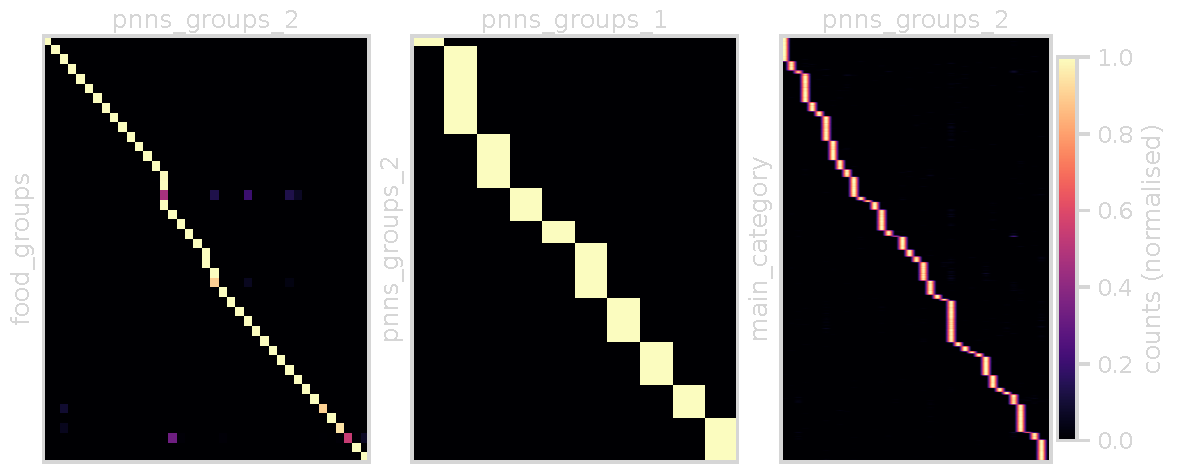
\includegraphics[width=90mm]{groups_mapping.pdf}
			} ;
		}

	\end{tikzpicture}
\end{frame}

\begin{frame}[t, label=diagramEnergy]
	\vfill
	\begin{center}
	\begin{tikzpicture}
		\linespread{1}% <--- locally defined vertical line spacing in nodes
		% \draw[clrBorders] (0,0) rectangle (\textwidth,\textheight) ;

		\begin{scope}[yshift=-10mm]
			\node[diagram0] (A) at (0.22\textwidth,0.9\textheight) {Data~set\\\textbf{initial}} ;

			\node[diagram0, right=of A] (B) {Gestion des \textbf{doublons}} ;
			\draw[myarrow] (A) -- (B) ;

			\node[diagram0, right=of B] (C) {Filtrages par \textbf{mots-clefs} / des \textbf{colonnes~vides}} ; % france + nom produit
			\draw[myarrow] (B) -- (C) ;

			\node[diagram0, below=of C] (D) {Gestion~des \textbf{valeurs aberrantes}} ;
			\draw[myarrow] (C) -- (D) ;

			\node[diagram0, left=of D] (E) {Remplissage grâce aux \textbf{données} \textbf{voisines}} ;
			\draw[myarrow] (D) -- (E) ;

			\node[text width=18mm, datavoisins, left=of E] (F) {Gestion de la variable \textbf{énergie}} ;
			\draw[myarrow] (E) -- (F) ;

			\node[diagram0, below=of F] (G) {Filtrages par \textbf{décompte} des \textbf{NaN}} ; % france + nom produit
			\draw[myarrow] (F) -- (G) ;

			\node[text width=18mm, diagram0, right=of G] (H) {Filtrage selon les \textbf{valeurs aberrantes}} ; % france + nom produit
			\draw[myarrow] (G) -- (H) ;

			\node[text width=18mm, diagram0, right=of H] (I) {Data~set\\\textbf{nettoyé}} ; % france + nom produit
			\draw[myarrow] (H) -- (I) ;
		\end{scope}

	\end{tikzpicture}
	\end{center}
	\vfill
\end{frame}

\begin{frame}[t, label=Energy]
	\vspace{0mm}
	\begin{tikzpicture}
		\draw[clrBorders] (0,0) rectangle (\textwidth,\textheight) ;

		\node[text centered, text width=80mm] at (0.5\textwidth,0.88\textheight)
			{Présence de \alert{valeurs incohérentes}:\\idéalement $x$ en kJ, $y$ en kcal et $y$$\approx$$\frac{900}{3700}x$} ;

		\begin{scope}[xshift=0.47\textwidth, yshift=0.5\textheight]
			\visible<1>{
				\node at (0,0) {
					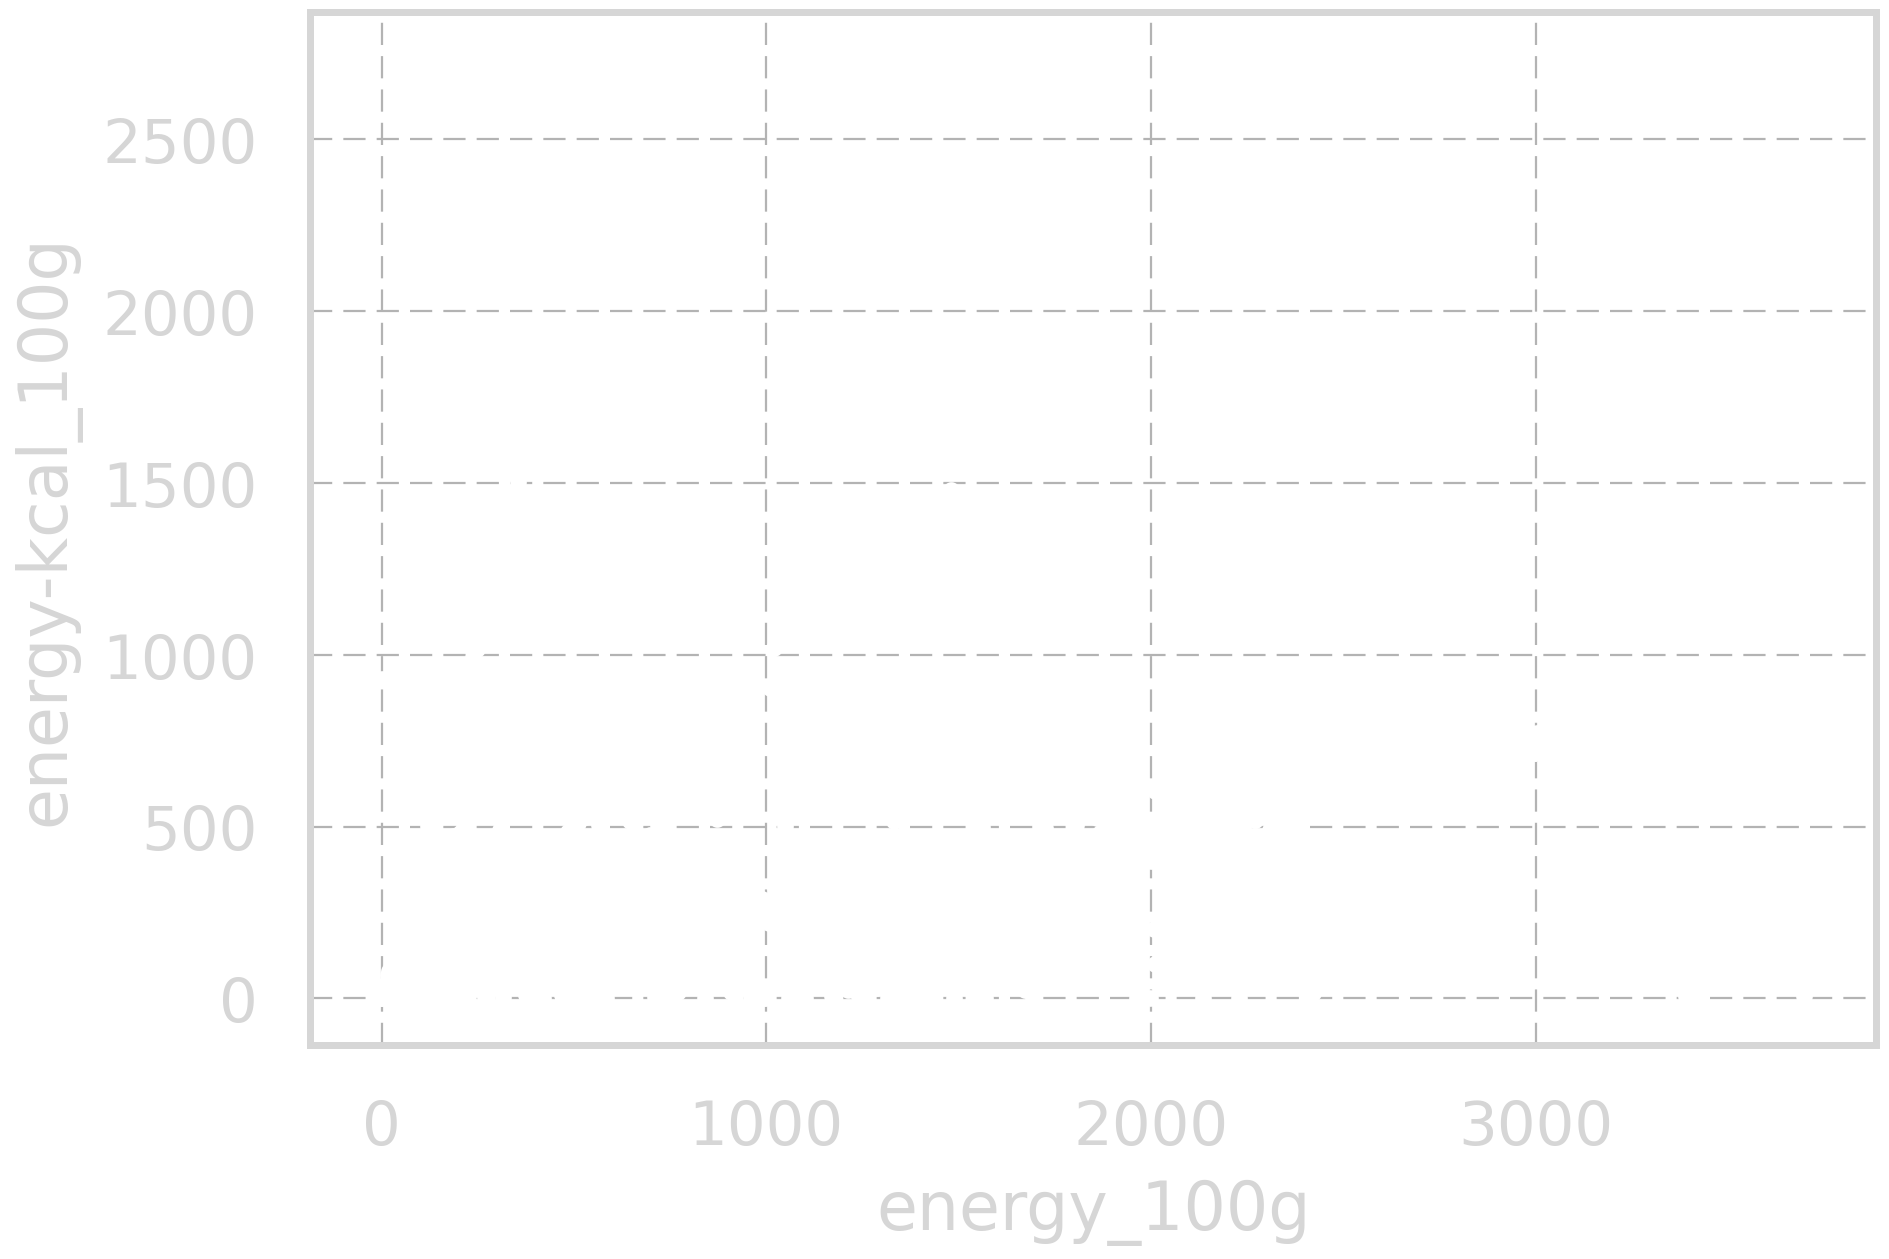
\includegraphics[width=80mm]{Energy-0.png}
					} ;
			}
			\visible<2>{
				\node at (0,0) {
					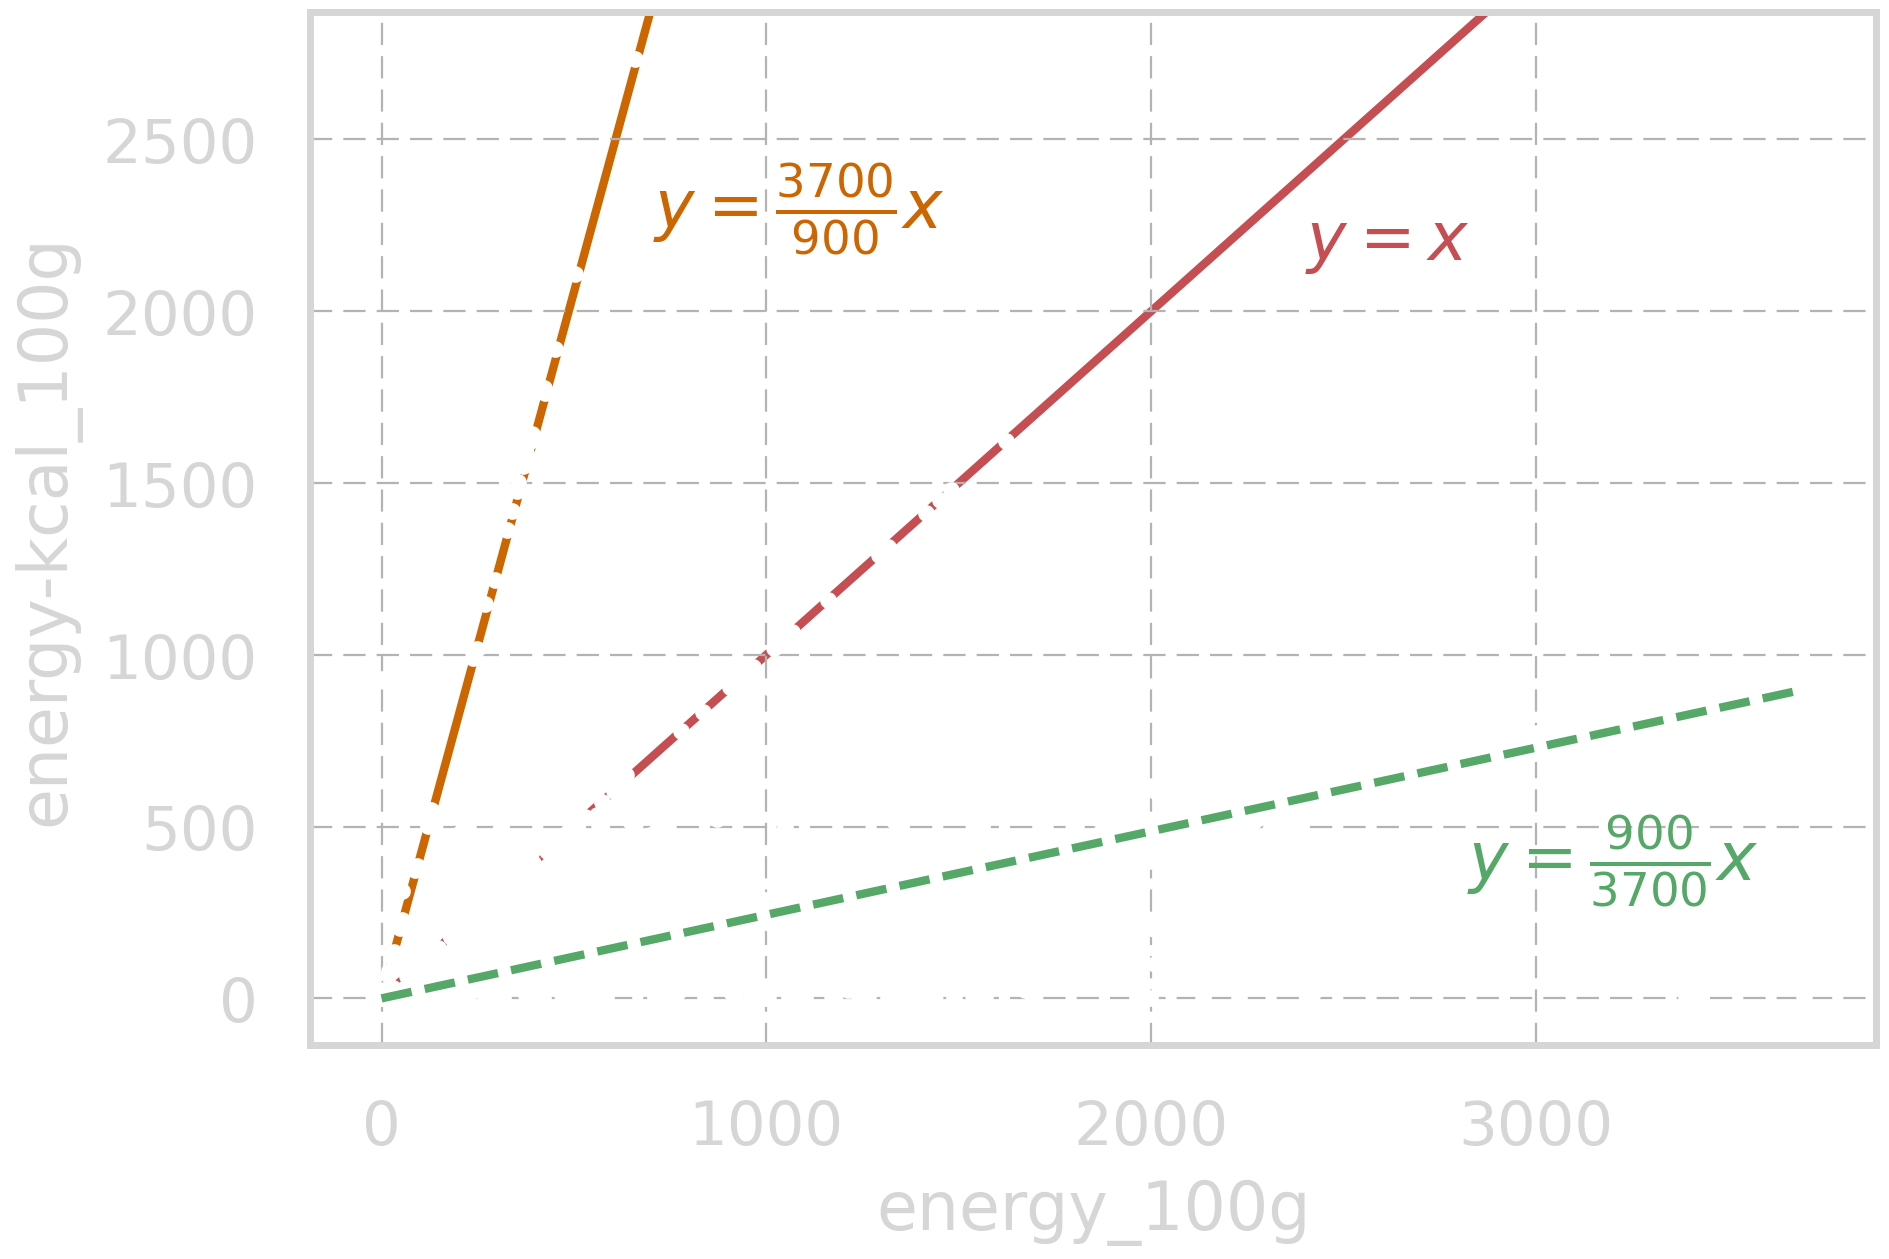
\includegraphics[width=80mm]{Energy-1.png}
					} ;
			}
			\visible<3->{
				\node at (0,0) {
					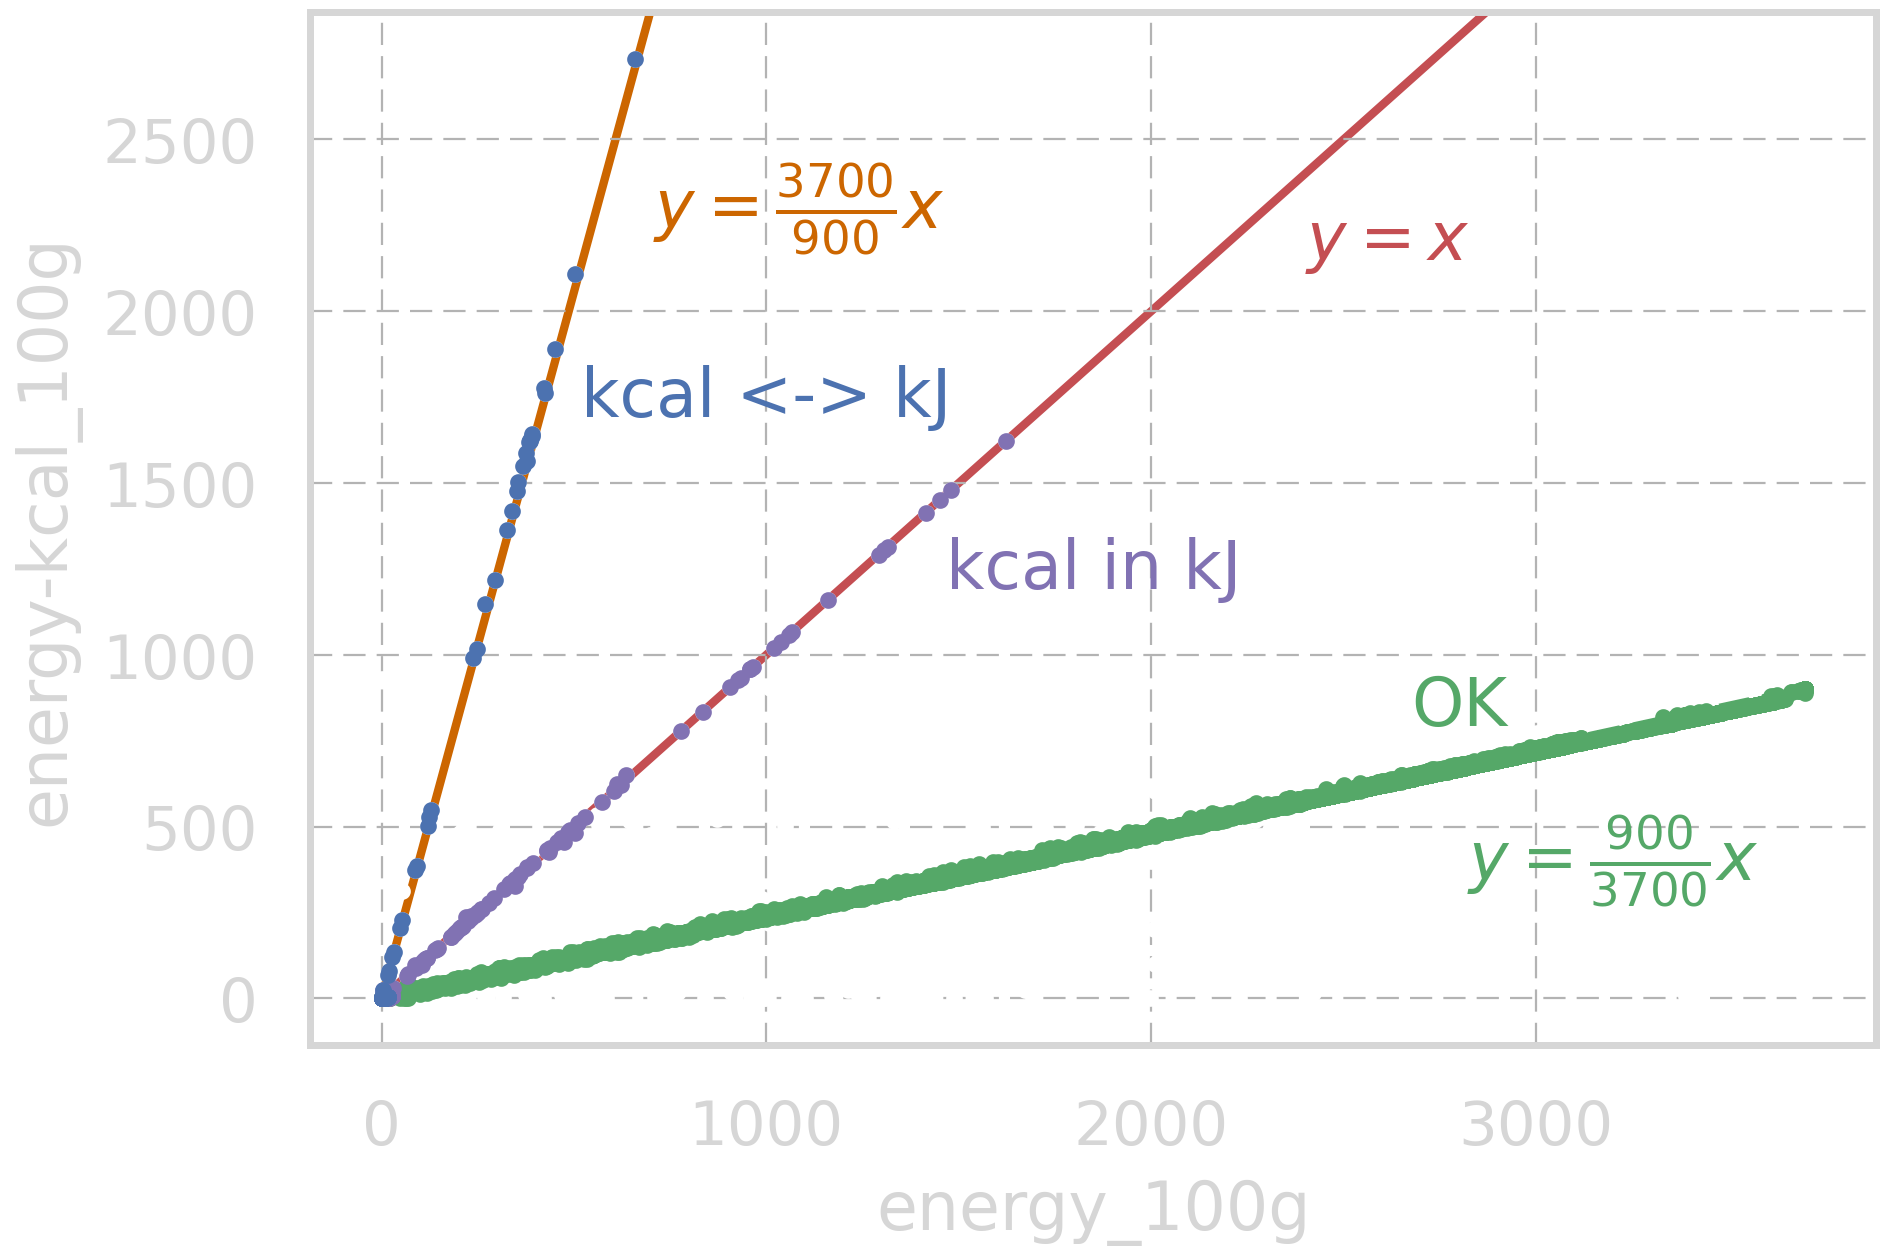
\includegraphics[width=80mm]{Energy-2.png}
					} ;
			}
		\end{scope}

		\visible<4>{
			\node[anchor=center, text centered] (B) at (0.5\textwidth,0.12\textheight) {Solution: garder la \alert{valeur maximale} (en kJ)} ;
			% \node[left=of B, xshift=2mm] (A) {} ;
			% \draw[myarrow, ultra thick, line width=1.2mm] (A) -- (B) ;
			% \draw[black, line width=.6mm] (A) -- ++ (6.2mm,0) ;
			% \node[right=of B.east, xshift=20mm, anchor=center] (C) at (0.5\textwidth,0.18\textheight) {\alert{energy-kj}} ;
			% \draw[myarrow, thick] (B) -- (C) ;
		}

	\end{tikzpicture}
\end{frame}




\begin{frame}[t, label=diagramFiltrageNaN]
	\vfill
	\begin{center}
	\begin{tikzpicture}
		\linespread{1}% <--- locally defined vertical line spacing in nodes
		% \draw[clrBorders] (0,0) rectangle (\textwidth,\textheight) ;

		\begin{scope}[yshift=-10mm]
			\node[diagram0] (A) at (0.22\textwidth,0.9\textheight) {Data~set\\\textbf{initial}} ;

			\node[diagram0, right=of A] (B) {Gestion des \textbf{doublons}} ;
			\draw[myarrow] (A) -- (B) ;

			\node[diagram0, right=of B] (C) {Filtrages par \textbf{mots-clefs} / des \textbf{colonnes~vides}} ; % france + nom produit
			\draw[myarrow] (B) -- (C) ;

			\node[diagram0, below=of C] (D) {Gestion~des \textbf{valeurs aberrantes}} ;
			\draw[myarrow] (C) -- (D) ;

			\node[diagram0, left=of D] (E) {Remplissage grâce aux \textbf{données} \textbf{voisines}} ;
			\draw[myarrow] (D) -- (E) ;

			\node[diagram0, left=of E] (F) {Gestion de la variable \textbf{énergie}} ;
			\draw[myarrow] (E) -- (F) ;

			\node[text width=18mm, filtrage, below=of F] (G) {Filtrages par \textbf{décompte} des \textbf{NaN}} ; % france + nom produit
			\draw[myarrow] (F) -- (G) ;

			\node[text width=18mm, diagram0, right=of G] (H) {Filtrage selon les \textbf{valeurs aberrantes}} ; % france + nom produit
			\draw[myarrow] (G) -- (H) ;

			\node[text width=18mm, diagram0, right=of H] (I) {Data~set\\\textbf{nettoyé}} ; % france + nom produit
			\draw[myarrow] (H) -- (I) ;
		\end{scope}

	\end{tikzpicture}
	\end{center}
	\vfill
\end{frame}

\begin{frame}[t, label=FiltrageNaN]
	\vspace{0mm}
	\begin{tikzpicture}
		\linespread{1}% <--- locally defined vertical line spacing in nodes
		\draw[clrBorders] (0,0) rectangle (\textwidth,\textheight) ;

		\node[text width=15mm]
			(A) at (0.2\textwidth,0.8\textheight)  {} ;

		\visible<2->{
			\node[box_style00, text width=25mm, right=of A] (B) { Filtrage:\\décompte des NaN > 10\% } ;
			\draw[myarrow] (A.center) -- (B) ;
		}
		\node[text width=15mm, right=of B] (C) { } ;


		\filldraw[clrData] (A.center) circle (5mm) ;
		\node[text centered, font=\bfseries\fontsize{10}{10}\selectfont]
			at (A.center) {108} ;
		\node[below=of A, yshift=6mm] {\small \textit{variables}} ;




		\visible<3->{
			\filldraw[clrData] (C.center) circle (5mm) ;
			\node[text centered, font=\bfseries\fontsize{10}{10}\selectfont]
				at (C.center) {33} ;
			\node[below=of C, yshift=6mm] {\small \textit{variables}} ;
		\draw[myarrow] (B.east) -- ++ (13.5mm,0) ;
		}

		\visible<4->{
		\node at (0.5\textwidth,0.63\textheight) {Taux de \alert{remplissage} des \alert{variables sélectionnées}:} ;
		\node at (0.5\textwidth,0.3\textheight)
			{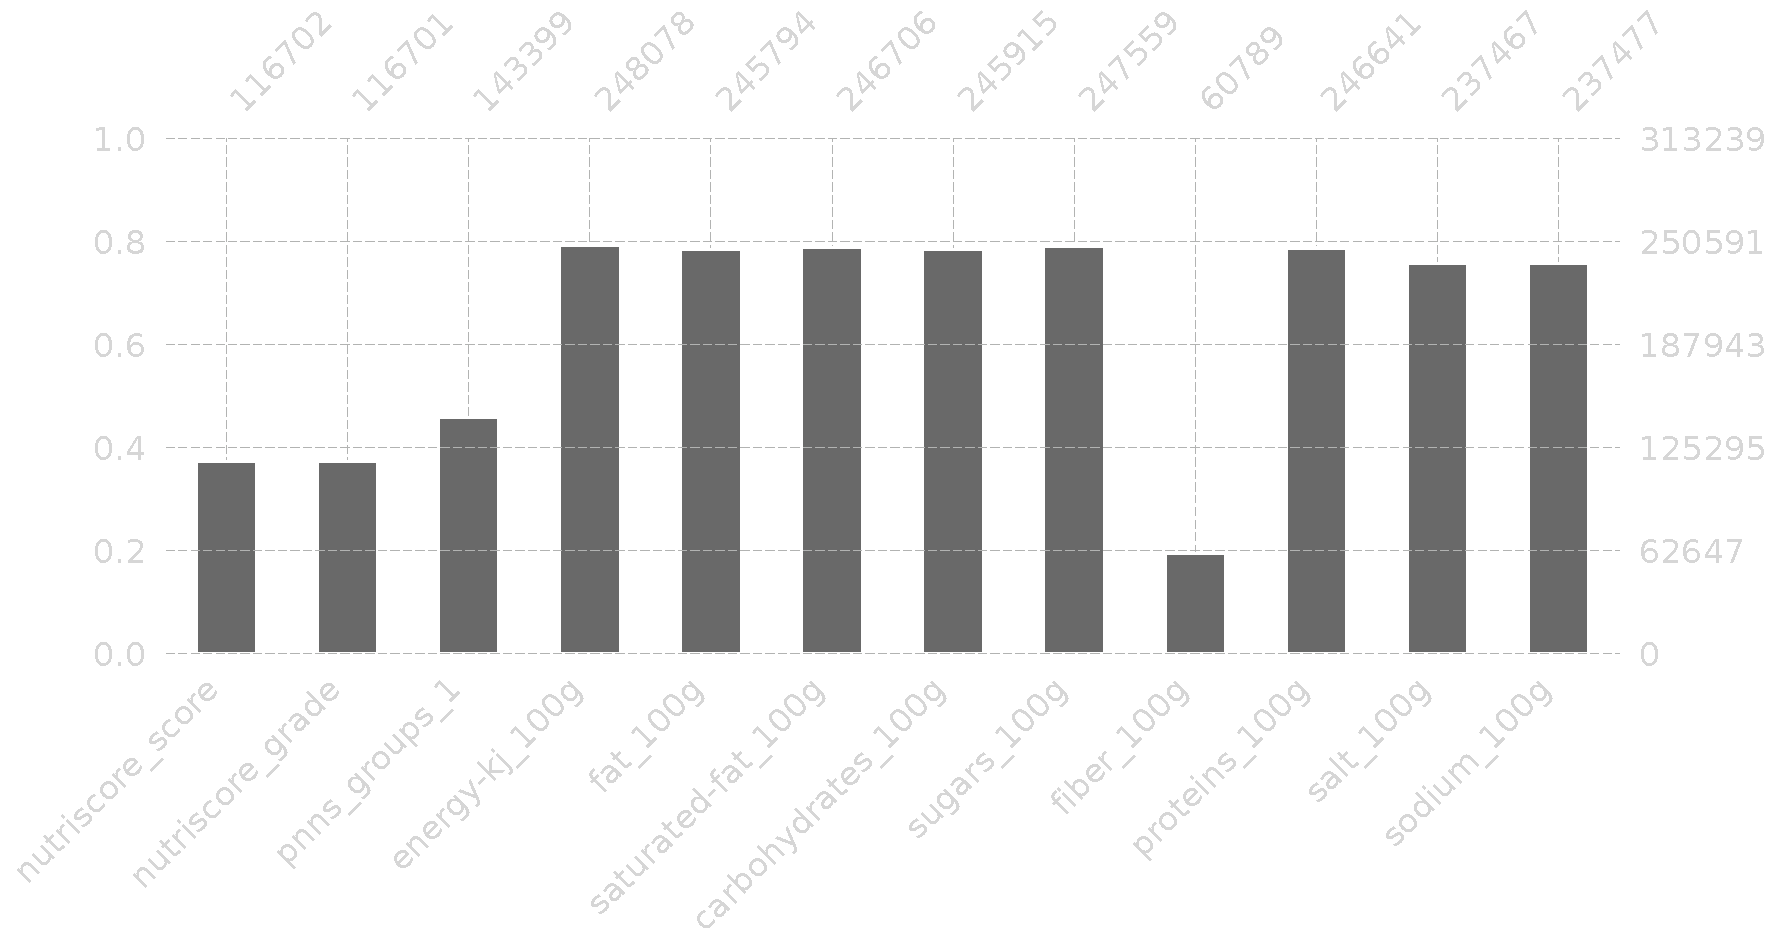
\includegraphics[width=90mm]{bar_NaN.pdf}} ;
		}
		\visible<5->{
		\begin{scope}[xshift=66.74mm, yshift=17.5mm]
			\draw[myOrng, rounded corners, thick] (0,0) rectangle (6mm, 26mm) ;
		\end{scope}
		\node[myOrng, draw, thick, rounded corners, font=\bfseries, fill=black, opacity=0.5] (D) at (41.5mm, 41.9mm) {\phantom{Remplacement des NaN avec des 0}} ;
		\node[myOrng, draw, thick, rounded corners, font=\bfseries] at (D.center) {Remplacement des NaN avec des 0} ;
		}
	\end{tikzpicture}
\end{frame}


\begin{frame}[t, label=FiltrageNaN2]
	\vspace{0mm}
	\begin{tikzpicture}
		\linespread{1}% <--- locally defined vertical line spacing in nodes
		\draw[clrBorders] (0,0) rectangle (\textwidth,\textheight) ;

		\node[text width=60mm, text centered] at (0.5\textwidth,0.9\textheight) {Matrice de \alert{remplissage} des \alert{variables sélectionnées}:\\(tri ascendant des valeurs)} ;
		\node at (0.5\textwidth,0.47\textheight)
			{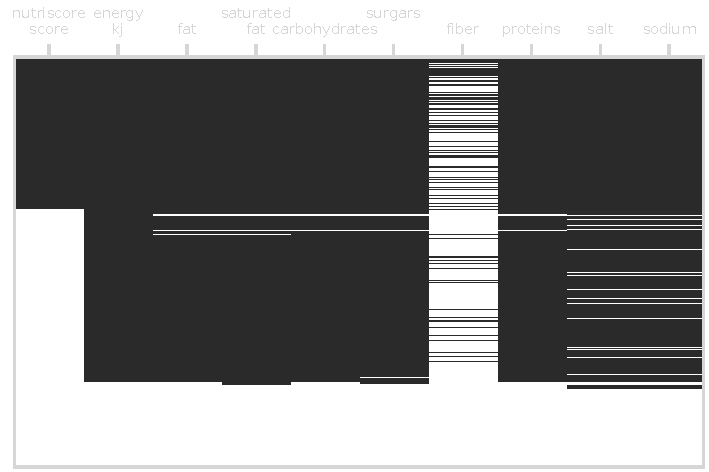
\includegraphics[width=90mm]{matrix_NaN.pdf}} ;

		\visible<2->{
		\node[myOrng, text centered, font=\bfseries] at (44mm, 58mm) {Valeurs remplies} ;
		}
		\visible<3->{
		\node[myOrng, text centered, font=\bfseries] at (0.5\textwidth, 19mm) {Valeurs NaN} ;
		}

		\visible<4->{
		\begin{scope}[xshift=10mm, yshift=12.5mm]
			\draw[myOrng, rounded corners, thick] (0,0) rectangle (90mm, 11.5mm) ;
		\end{scope}
		\node[text centered] at (0.5\textwidth, 8mm) {\alert{Suppression} des \alert{entrées vides}} ;
		}
	\end{tikzpicture}
\end{frame}



\begin{frame}[t, label=diagramFiltrageValAberrantes]
	\vfill
	\begin{center}
	\begin{tikzpicture}
		\linespread{1}% <--- locally defined vertical line spacing in nodes
		% \draw[clrBorders] (0,0) rectangle (\textwidth,\textheight) ;

		\begin{scope}[yshift=-10mm]
			\node[diagram0] (A) at (0.22\textwidth,0.9\textheight) {Data~set\\\textbf{initial}} ;

			\node[diagram0, right=of A] (B) {Gestion des \textbf{doublons}} ;
			\draw[myarrow] (A) -- (B) ;

			\node[diagram0, right=of B] (C) {Filtrages par \textbf{mots-clefs} / des \textbf{colonnes~vides}} ; % france + nom produit
			\draw[myarrow] (B) -- (C) ;

			\node[diagram0, below=of C] (D) {Gestion~des \textbf{valeurs aberrantes}} ;
			\draw[myarrow] (C) -- (D) ;

			\node[diagram0, left=of D] (E) {Remplissage grâce aux \textbf{données} \textbf{voisines}} ;
			\draw[myarrow] (D) -- (E) ;

			\node[diagram0, left=of E] (F) {Gestion de la variable \textbf{énergie}} ;
			\draw[myarrow] (E) -- (F) ;

			\node[text width=18mm, diagram0, below=of F] (G) {Filtrages par \textbf{décompte} des \textbf{NaN}} ; % france + nom produit
			\draw[myarrow] (F) -- (G) ;

			\node[text width=18mm, filtrage, right=of G] (H) {Filtrage selon les \textbf{valeurs aberrantes}} ; % france + nom produit
			\draw[myarrow] (G) -- (H) ;

			\node[text width=18mm, diagram0, right=of H] (I) {Data~set\\\textbf{nettoyé}} ; % france + nom produit
			\draw[myarrow] (H) -- (I) ;
		\end{scope}

	\end{tikzpicture}
	\end{center}
	\vfill
\end{frame}


\begin{frame}[t, label=SumWeight]
	\vspace{0mm}
	\begin{tikzpicture}
		\linespread{1}% <--- locally defined vertical line spacing in nodes
		\draw[clrBorders] (0,0) rectangle (\textwidth,\textheight) ;

		\node at (0.5\textwidth,0.92\textheight) {Calcul de la \alert{somme} des \alert{macro-nutriments}} ;
		\visible<2->{
		\node at (0.5\textwidth,0.86\textheight) {Données \alert{statistiques} sur les \alert{données brutes}:} ;

			\node at (0.5\textwidth,0.8\textheight) {
				\begin{tabular}{ccccccccc}
					\rowcolor{dfFirstRow}
					& count & mean & std & min & 25\% & 50\% & 75\% & max \tabularnewline
					\rowcolor{dfEvenRow}
					$\sum$ poids & 244025 & 51.27 & 31.43 & 0 & 23.8 & 47.5 & 83.9 & 300
				\end{tabular}
			} ;
		}

		\visible<3->{
		\node at (0.5\textwidth,0.61\textheight) {
			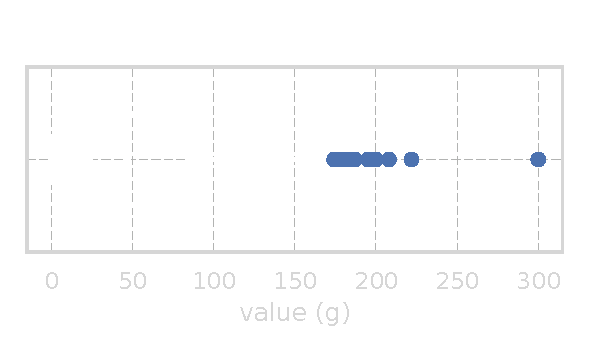
\includegraphics[width=50mm]{sumWeights_box.pdf}
		} ;
		}

		\visible<4->{
			\node[box_style00, draw, text width=40mm, text centered] (Q3IQ) at (0.25\textwidth,0.35\textheight) {
			Q3+1.5*IQ = \alert{174.05}\\$\rightarrow$ 12 outliers\\
			% vmax = 100 $\rightarrow$ 1651 outliers
		} ;
		}

		\visible<7->{
			\node[myOrng, very thick,box_style00, draw, text width=40mm, text centered] (VMAX100) at (0.25\textwidth,0.2\textheight) {
			% Q3+1.5*IQ = 174.05\\$\rightarrow$ 12 outliers\\
			vmax = 100\\$\rightarrow$ \alert{1651} outliers
		} ;
		\draw[myarrow] (Q3IQ) -- (VMAX100) ;
		}

		\visible<5->{
		\node at (0.74\textwidth,0.25\textheight) {
			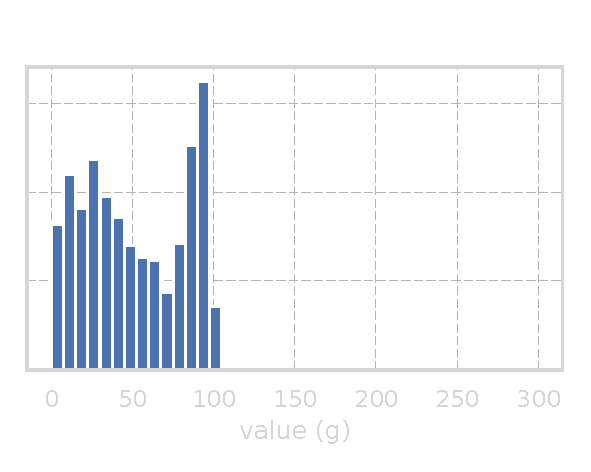
\includegraphics[width=50mm]{sumWeights_histo.pdf}
		} ;
		}
		\visible<6->{
			\node[myOrng, font=\bfseries, text centered] (2MODES) at (0.835\textwidth,0.33\textheight) {2 modes} ;
			\draw[myarrow, myOrng] (2MODES) -- (73mm, 33mm) ;
			\draw[myarrow, myOrng] (2MODES) -- (64mm, 28mm) ;
		}


	\end{tikzpicture}
\end{frame}


\section{EXPLORATION DES DONNÉES}



\subsection{Remplissage des valeurs NaN éparses}

\begin{frame}[t, label=fillMean]
	\vspace{0mm}
	\begin{tikzpicture}
		\linespread{1}% <--- locally defined vertical line spacing in nodes
		\draw[clrBorders] (0,0) rectangle (\textwidth,\textheight) ;

		\node at (0.4\textwidth,0.92\textheight) {Méthode 1: Valeur moyenne par pnns groups et par variable} ;

		\visible<2->{
		\node[box_style00, text width=35mm, minimum height=12mm] (A) at (0.25\textwidth,0.8\textheight) (A) {Calcul de la \alert{valeur moyenne} par pnns groups} ;
		}

		\visible<3->{
		\node[box_style00, text width=35mm, minimum height=12mm] (B) at (0.75\textwidth,0.8\textheight) (B) {Remplacement des \alert{NaN} par la \alert{valeur moyenne} par pnns groups} ;
		\draw[myarrow] (A) -- (B) ;
		}

		% \node[text width=70mm] at (0.5\textwidth,0.8\textheight)
		% {- Calcul valeur moyenne par pnns group et par variable\\- remplacement des NaN selon pnns group et variable\\- distribution non-gaussiennes\\- changement distribution si +sieurs modes et beaucoup de NaN} ;

		\visible<4->{
		\node at (0.32\textwidth,0.36\textheight) {
			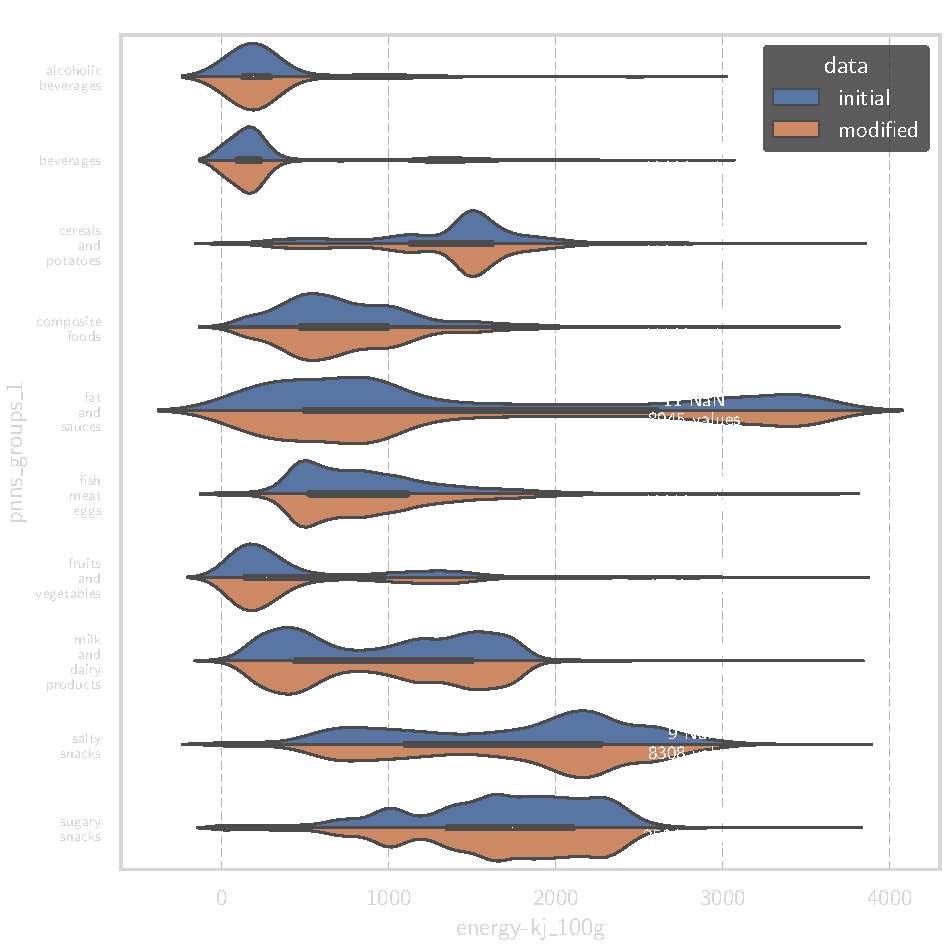
\includegraphics[width=60mm]{fillMean/energy-kj_100g.pdf}
		} ;
		}

		% \visible<5->{
		% 	\draw[myOrng, thick] (35.5mm,36.5mm) circle (3mm) ;
		% 	\node[myOrng, font=\fontsize{6}{6}\selectfont\bfseries, text centered] at (50.7mm,39.7mm) {2 modes et 12\% de NaN} ;
		% }

		\visible<5->{
			\node[anchor=west] at (0.64\textwidth,0.6\textheight) {$\bullet$ variations imperceptibles} ;
			\node[anchor=west] at (0.64\textwidth,0.55\textheight) {$\bullet$ distribution \alert{multi-modale}} ;
		}
		\visible<6->{
			\node[myOrng, very thick, box_style00, text width=20mm] (CCL) at (0.8\textwidth,0.4\textheight) {Méthode \alert{non adaptée} aux données} ;
			\draw[myarrow] (70.8mm,48mm) |- (CCL) ;
		}

	\end{tikzpicture}
\end{frame}




\begin{frame}[t, label=fillImputer]
	\vspace{0mm}
	\begin{tikzpicture}
		\linespread{1}% <--- locally defined vertical line spacing in nodes
		\draw[clrBorders] (0,0) rectangle (\textwidth,\textheight) ;

		\node at (0.5\textwidth,0.92\textheight) {Méthode 2: itérative imputer de la librairie Scikit-learn, basée sur une approche k-nn} ;

		\visible<2->{
		\node[box_style00, text width=30mm, minimum height=12mm] (A) at (0.25\textwidth,0.8\textheight) (A) {Apprentissage sur des\\\alert{données complètes}} ;
		}

		\visible<3->{
		\node[box_style00, text width=30mm, minimum height=12mm] (B) at (0.75\textwidth,0.8\textheight) (B) {Remplissage des \alert{données incomplètes}} ;
		\draw[myarrow] (A) -- (B) ;
		}

		% \node[text width=70mm] at (0.5\textwidth,0.8\textheight)
		% {- Calcul valeur moyenne par pnns group et par variable\\- remplacement des NaN selon pnns group et variable\\- distribution non-gaussiennes\\- changement distribution si +sieurs modes et beaucoup de NaN} ;

		\visible<4->{
		\node at (0.32\textwidth,0.36\textheight) {
			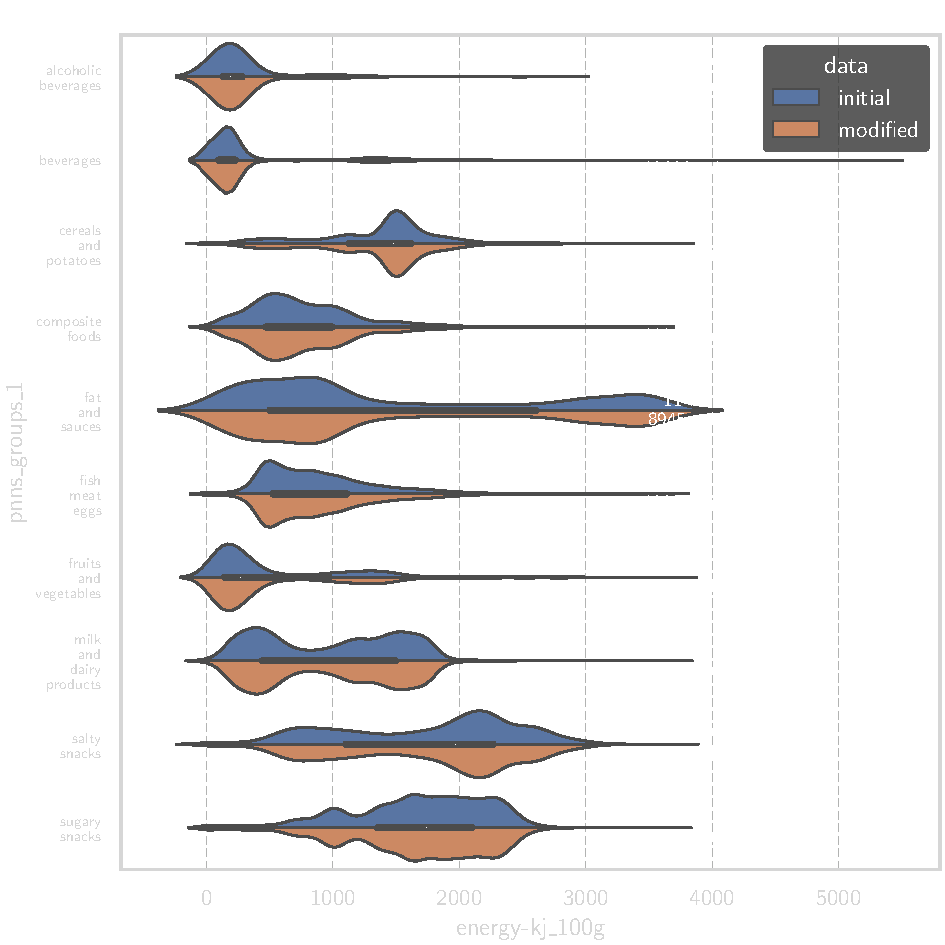
\includegraphics[width=60mm]{fillImputer/energy-kj_100g.pdf}
		} ;
		}

		\visible<5->{
			\draw[myOrng, thick] (54.5mm,52.7mm) circle [x radius=8mm, y radius=3mm] ;
			% \draw[myOrng, thick] (47mm,36.5mm) circle (3mm) ;
			% \node[myOrng, font=\fontsize{6}{6}\selectfont\bfseries, text centered] at (50.7mm,39.7mm) {2 modes et 12\% de NaN} ;
		}

		\visible<6->{
			% \node[anchor=west, text width=36mm] at (0.64\textwidth,0.6\textheight) {$\bullet$ modification de la\\\phantom{$\bullet$} distribution \alert{fat and}\\\phantom{$\bullet$} \alert{sauces} à nouveau} ;
			\node[anchor=west, text width=36mm] at (0.64\textwidth,0.51\textheight) {$\bullet$ génération de \alert{valeurs}\\\phantom{$\bullet$} \alert{hors bornes}} ;
		}
		\visible<7->{
			\node[myOrng, very thick, box_style00, text width=20mm] (CCL) at (0.8\textwidth,0.3\textheight) {Pour l'étude, \alert{suppression} des entrées \alert{incomplètes}} ;
			\draw[myarrow] (70.8mm,44.5mm) |- (CCL) ;
		}

	\end{tikzpicture}
\end{frame}


\subsection{Prédiction du nutriscore (remplissage des NaN)}


\begin{frame}[t, label=knnScaled]
	\vspace{0mm}
	\begin{tikzpicture}
		\linespread{1}% <--- locally defined vertical line spacing in nodes
		\draw[clrBorders] (0,0) rectangle (\textwidth,\textheight) ;

		\node[anchor=west] at (5mm,0.9\textheight) {{Principe:}} ;

		\begin{scope}[xshift=0.15\textwidth]
			\node[box_style00, text width=20mm] (A)
				at (0,0.75\textheight) {Données \alert{connues}} ;
				% at (0,0.75\textheight) {Calcul de la \alert{distance euclidienne} entre une \alert{entrée cible} et les \alert{entrée à sortie connue}} ;


			\visible<2->{
				\node[box_style00, text width=20mm] (B)
					at (0,0.4\textheight) {Entrée à \alert{sortie inconnue}} ;
			}

			\visible<3->{
				\node[box_style00, text width=20mm] (C)
					at (0,0.575\textheight) {Calcul des \alert{distances euclidiennes}} ;
				\draw[myarrow] (A) -- (C) ;
				\draw[myarrow] (B) -- (C) ;
			}
		\end{scope}

		\visible<4->{
			\node[box_style00, text width=20mm, anchor=center] (D)
				at (0.45\textwidth,0.75\textheight) {Sélection des \alert{k plus proches}} ;
			\draw[myarrow] (C) -| (D) ;
		}

		\visible<5->{
			\node[box_style00, text width=30mm, anchor=center] (E)
				at (0.8\textwidth,0.75\textheight) {Calcul de la \alert{valeur moyenne} pour les k éléments} ;
			\draw[myarrow] (D) -- (E) ;
		}

		\visible<6->{
		\node at (0.62\textwidth,0.35\textheight) {
			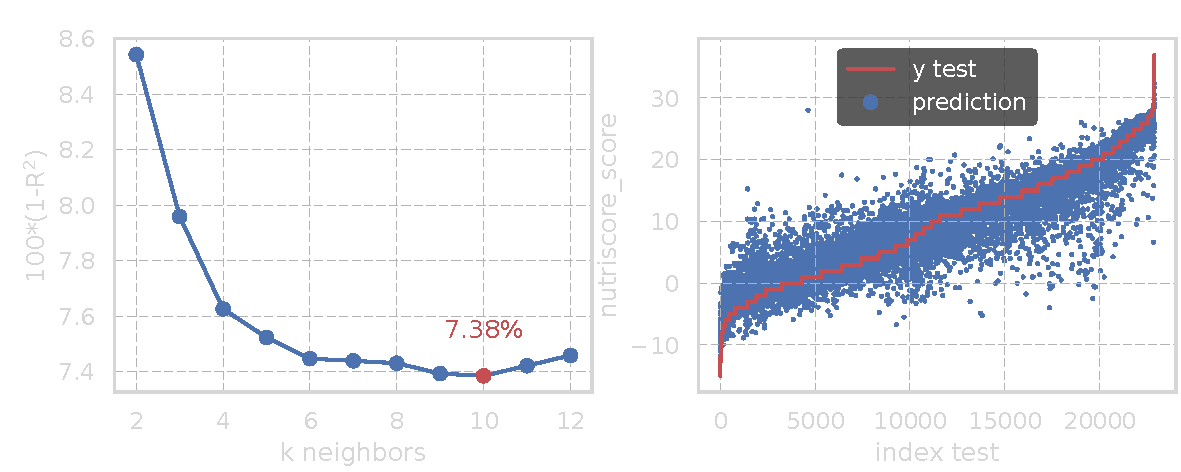
\includegraphics[width=78mm]{knn/2.pdf}
		} ;
		}

		\visible<7->{
			\node[text centered] at (0.5\textwidth,10mm) {Quid de l'\alert{hypothèse} NaN fibers = 0 ? } ;
		}

	\end{tikzpicture}
\end{frame}



\begin{frame}[t, label=knnFiber]
	\vspace{0mm}
	\begin{tikzpicture}
		\linespread{1}% <--- locally defined vertical line spacing in nodes
		\draw[clrBorders] (0,0) rectangle (\textwidth,\textheight) ;

		\node[anchor=west] at (5mm,0.9\textheight) {Vérification de l'hypothèse NaN fiber = 0:} ;

		\only<1->{
			\node at (0.48\textwidth,0.55\textheight) {
				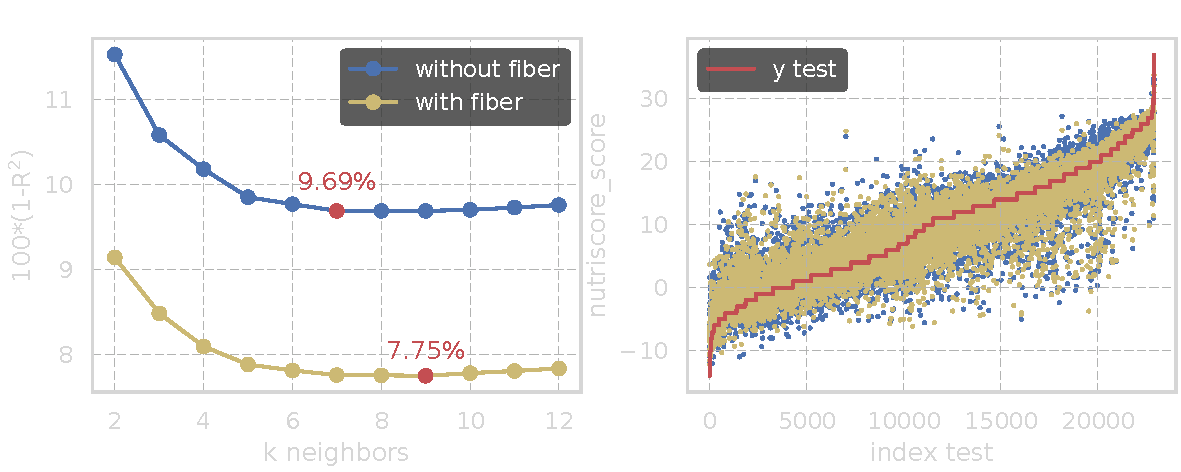
\includegraphics[width=90mm]{knn/3.pdf}
			} ;
		}
		\only<2->{
			\begin{scope}[yshift=-12mm]
				\node[anchor=west] at (0.2\textwidth,0.37\textheight) {$\rightarrow$ Hypothèse à priori \alert{validée} } ;
			\end{scope}
		}

	\end{tikzpicture}
\end{frame}


\subsection{Étude de l'inertie des valeurs - Analyse en Composantes Principales}
\begin{frame}[t, label=pca]
	\vspace{0mm}
	\begin{tikzpicture}
		\linespread{1}% <--- locally defined vertical line spacing in nodes
		\draw[clrBorders] (0,0) rectangle (\textwidth,\textheight) ;

		\node[anchor=west, text width=90mm] at (5mm,0.9\textheight) {Principe: Calcul des axes en vue d'\alert{aligner} les \alert{coordonnées} et les\\\alert{principaux axes d'inertie}} ;


		\only<2->{
			\node at (0.47\textwidth,0.55\textheight) {
				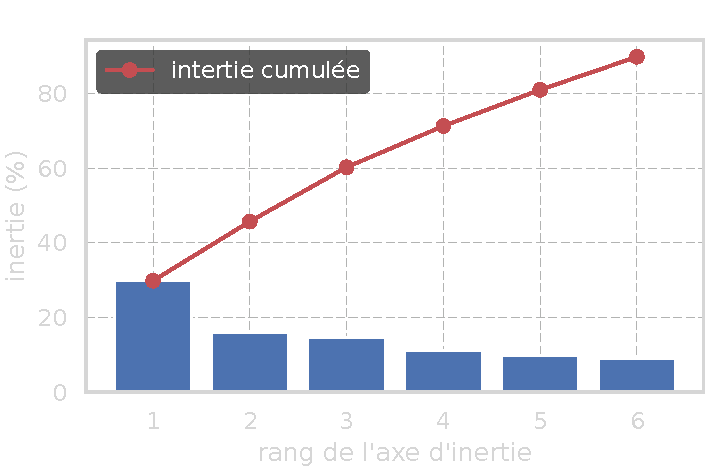
\includegraphics[width=60mm]{PCA/ebouli.pdf}
			} ;
		}

		\only<3>{
			\node[anchor=west] at (0.2\textwidth,20mm) {$\rightarrow$ \alert{90\%} de l'inertie sur \alert{6 axes}} ;
			\node[anchor=west] at (0.2\textwidth,16mm) {$\rightarrow$ Répartition relativement \alert{équilibrée}} ;
		}

	\end{tikzpicture}
\end{frame}

\begin{frame}[t, label=pca2]
	\vspace{0mm}
	\begin{tikzpicture}
		\linespread{1}% <--- locally defined vertical line spacing in nodes
		\draw[clrBorders] (0,0) rectangle (\textwidth,\textheight) ;

		\node[anchor=west, text width=90mm] at (5mm,0.9\textheight) {Projection des axes initiaux sur les axes estimés} ;


		\only<2>{
			\node at (0.47\textwidth,0.55\textheight) {
				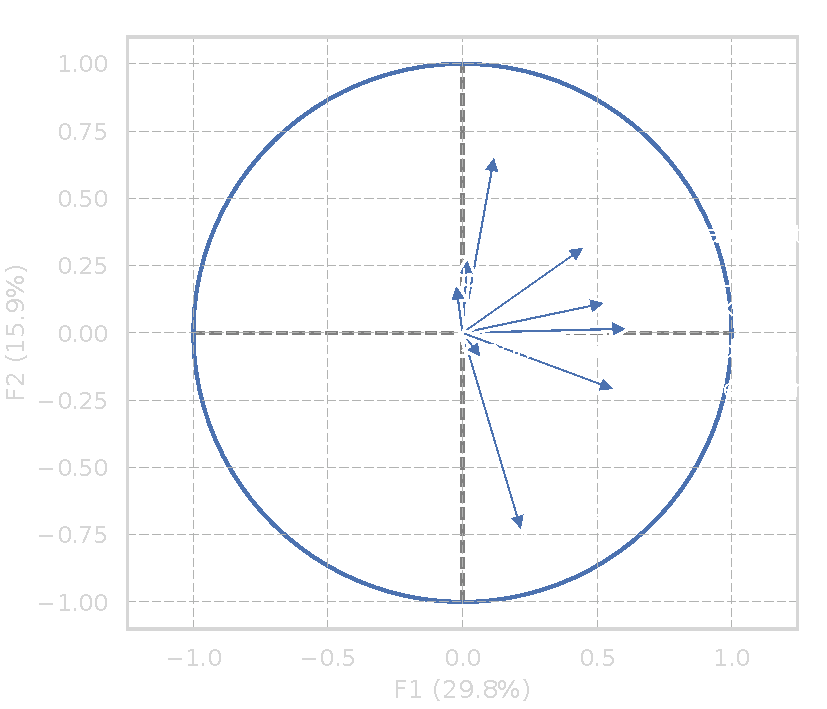
\includegraphics[width=60mm]{PCA/cercle-0.pdf}
			} ;
		}

		\only<3->{
			\node at (0.45\textwidth,0.65\textheight) {
				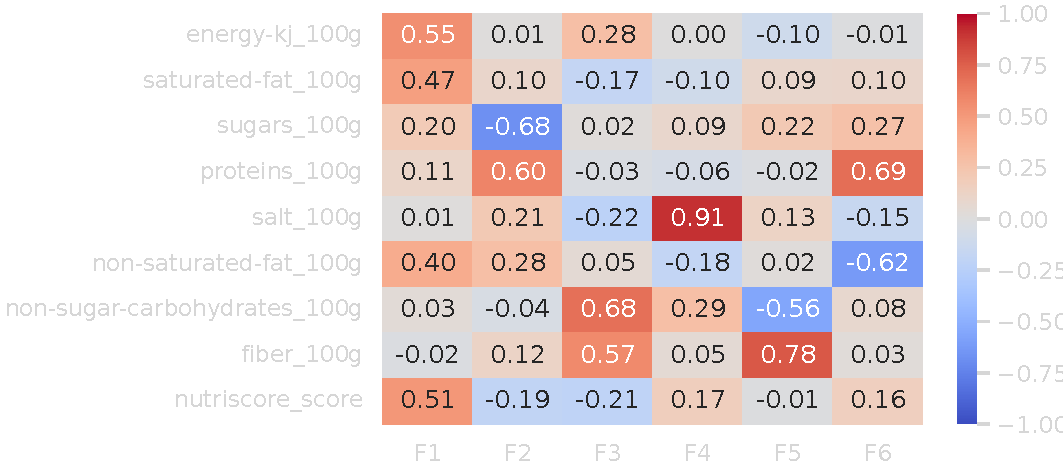
\includegraphics[width=60mm]{PCA/heatmap.pdf}
			} ;
			% \node[anchor=west] at (0.2\textwidth,20mm) {$\rightarrow$ \alert{90\%} de l'inertie sur \alert{6 axes}} ;
			% \node[anchor=west] at (0.2\textwidth,16mm) {$\rightarrow$ Répartition relativement \alert{équilibrée}} ;
		}

		\begin{scope}[xshift=0.5\textwidth, yshift=0.25\textheight]

			% \only<4>{
			% 	\node at (0,0) {
			% 		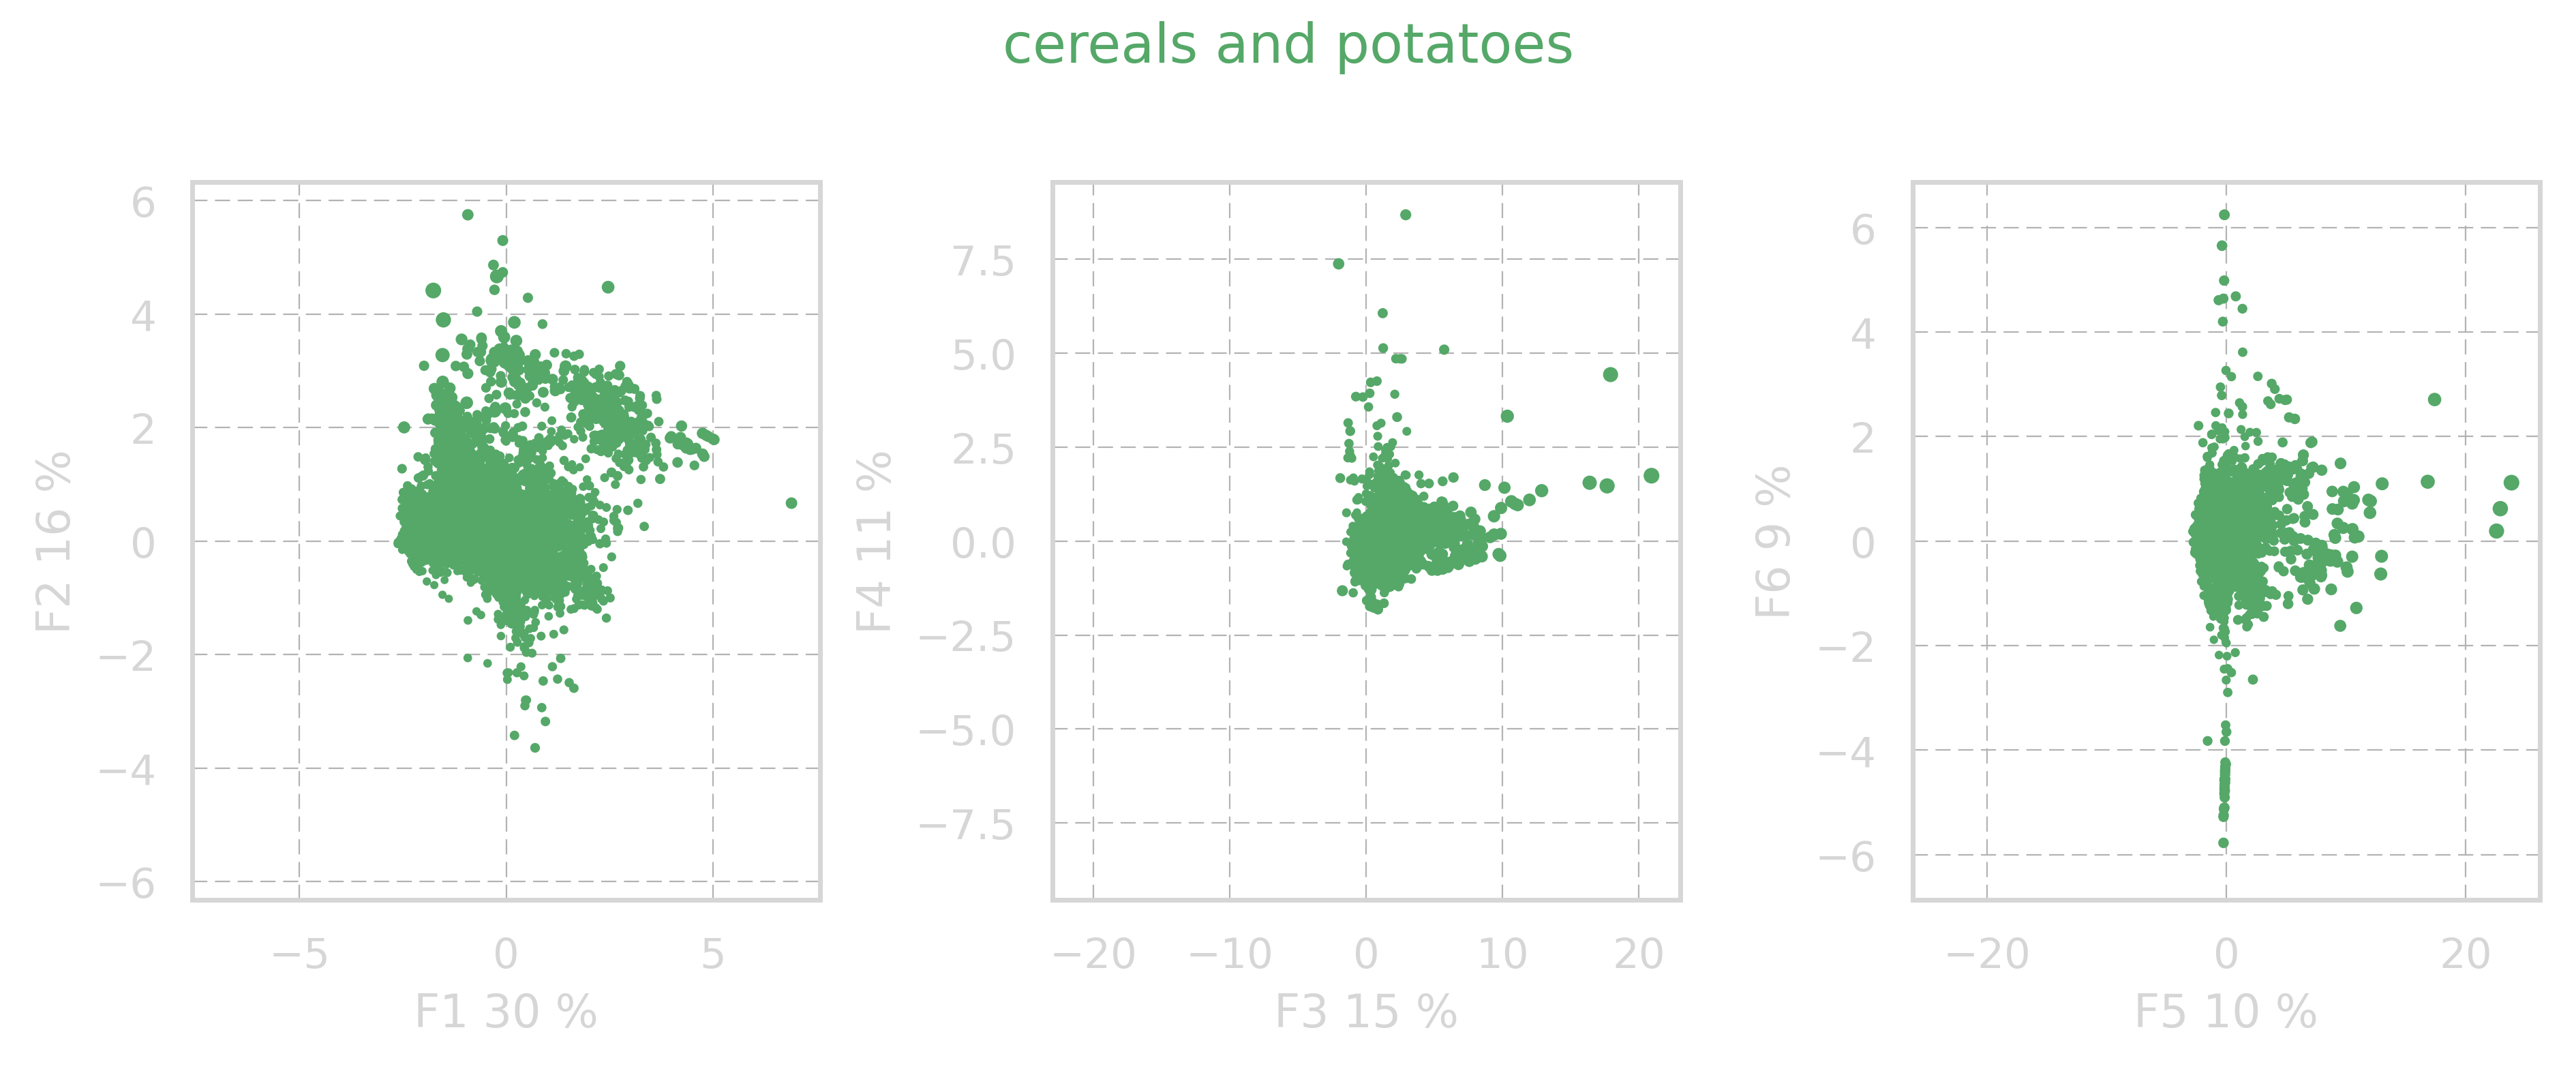
\includegraphics[width=80mm]{PCA/projection-cereals-and-potatoes.png}
			% 		} ;
			% 	}

			\only<4>{
				\node at (0,0) {
					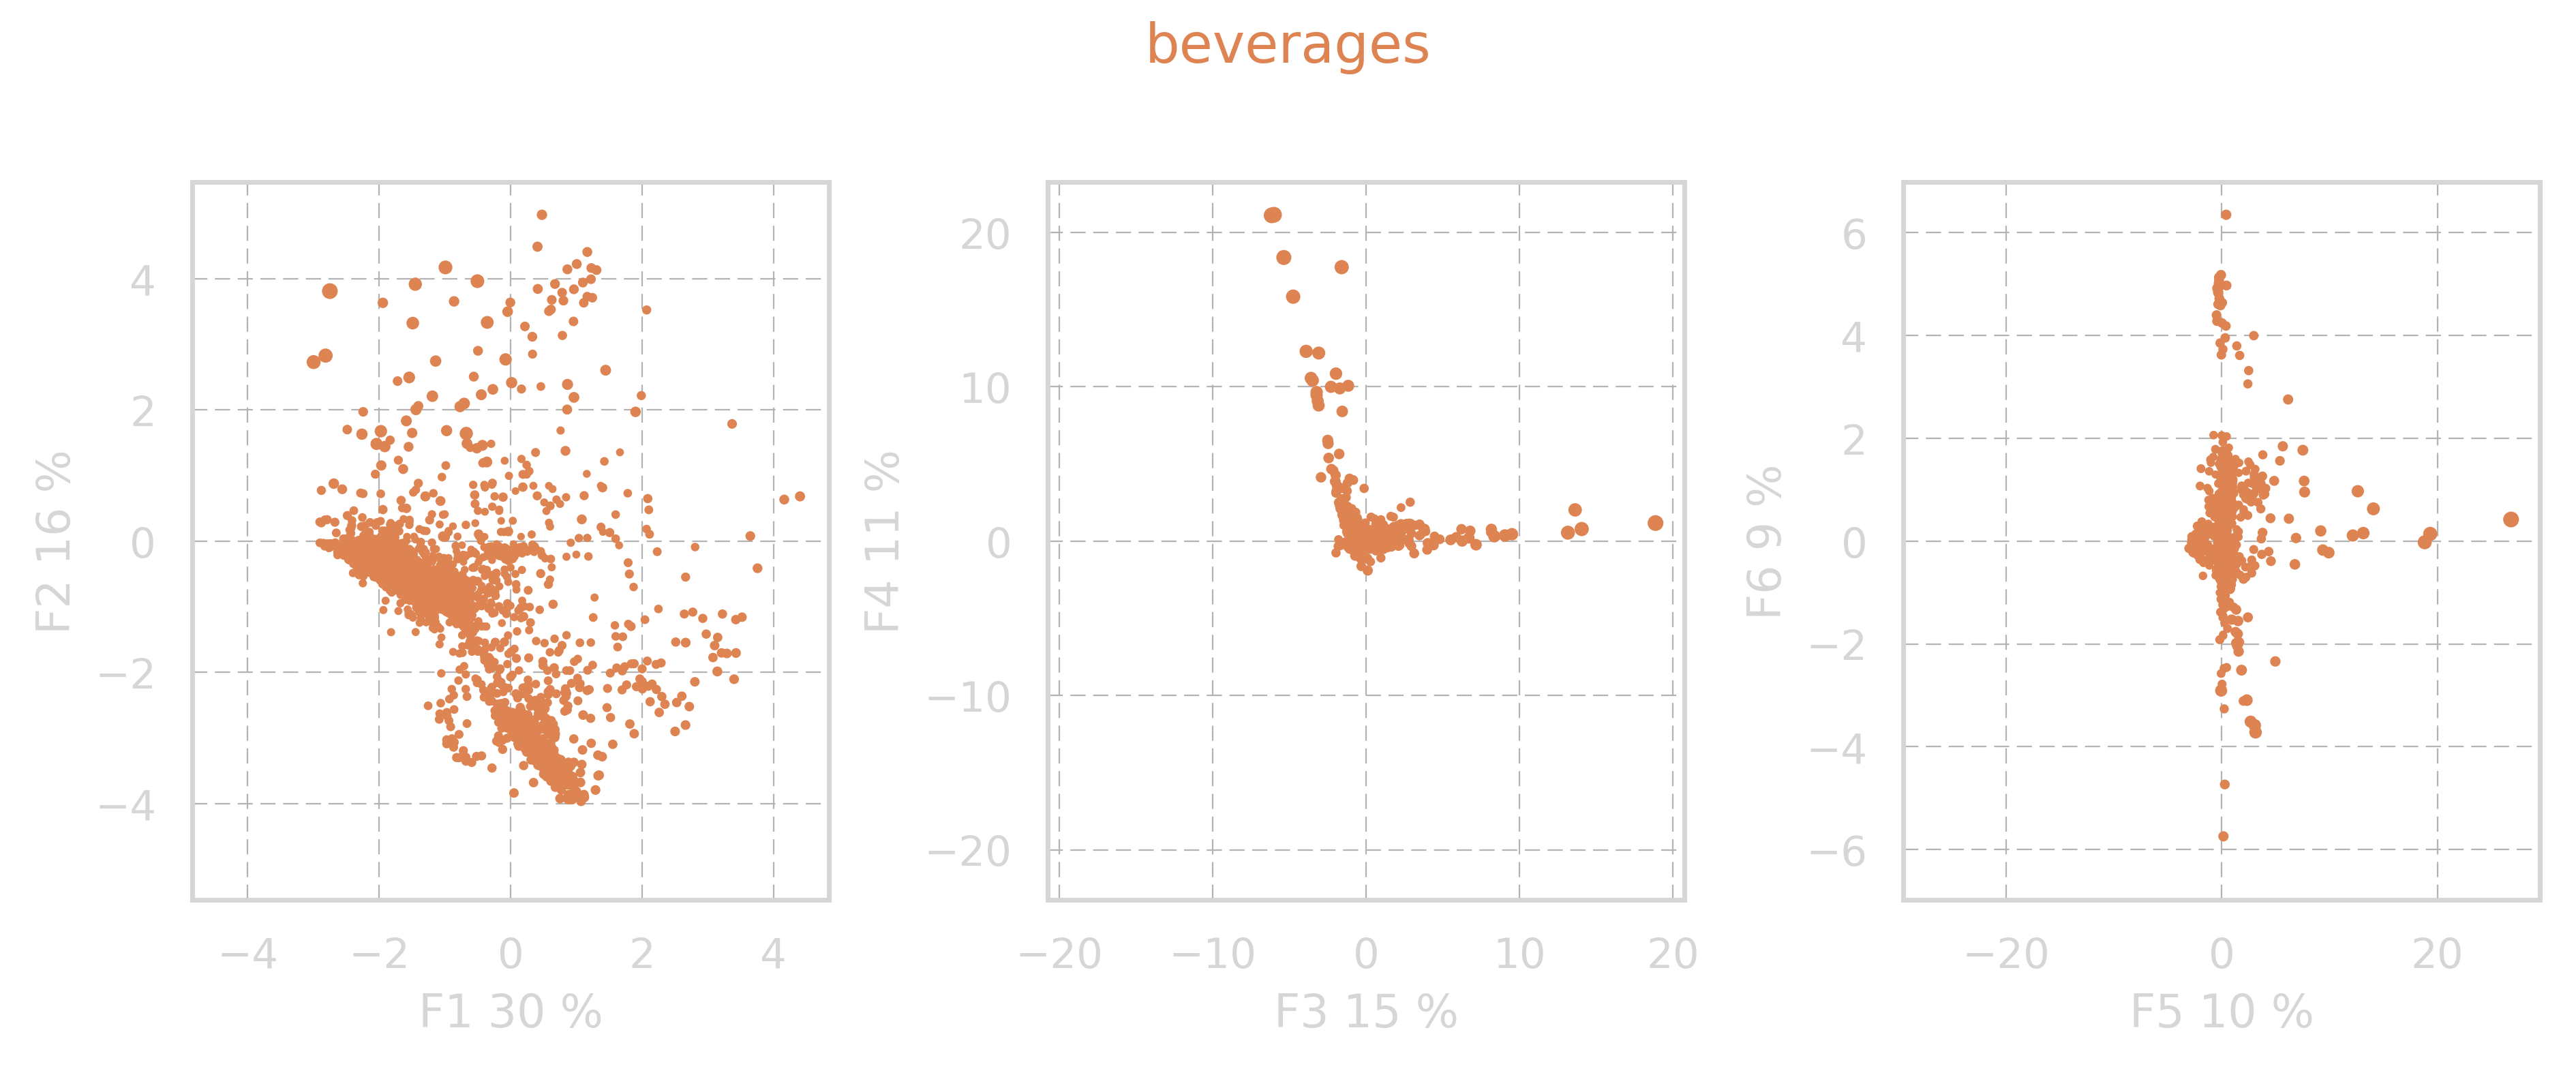
\includegraphics[width=80mm]{PCA/projection-beverages.png}
					} ;
				}

			% \only<6>{
			% 	\node at (0,0) {
			% 		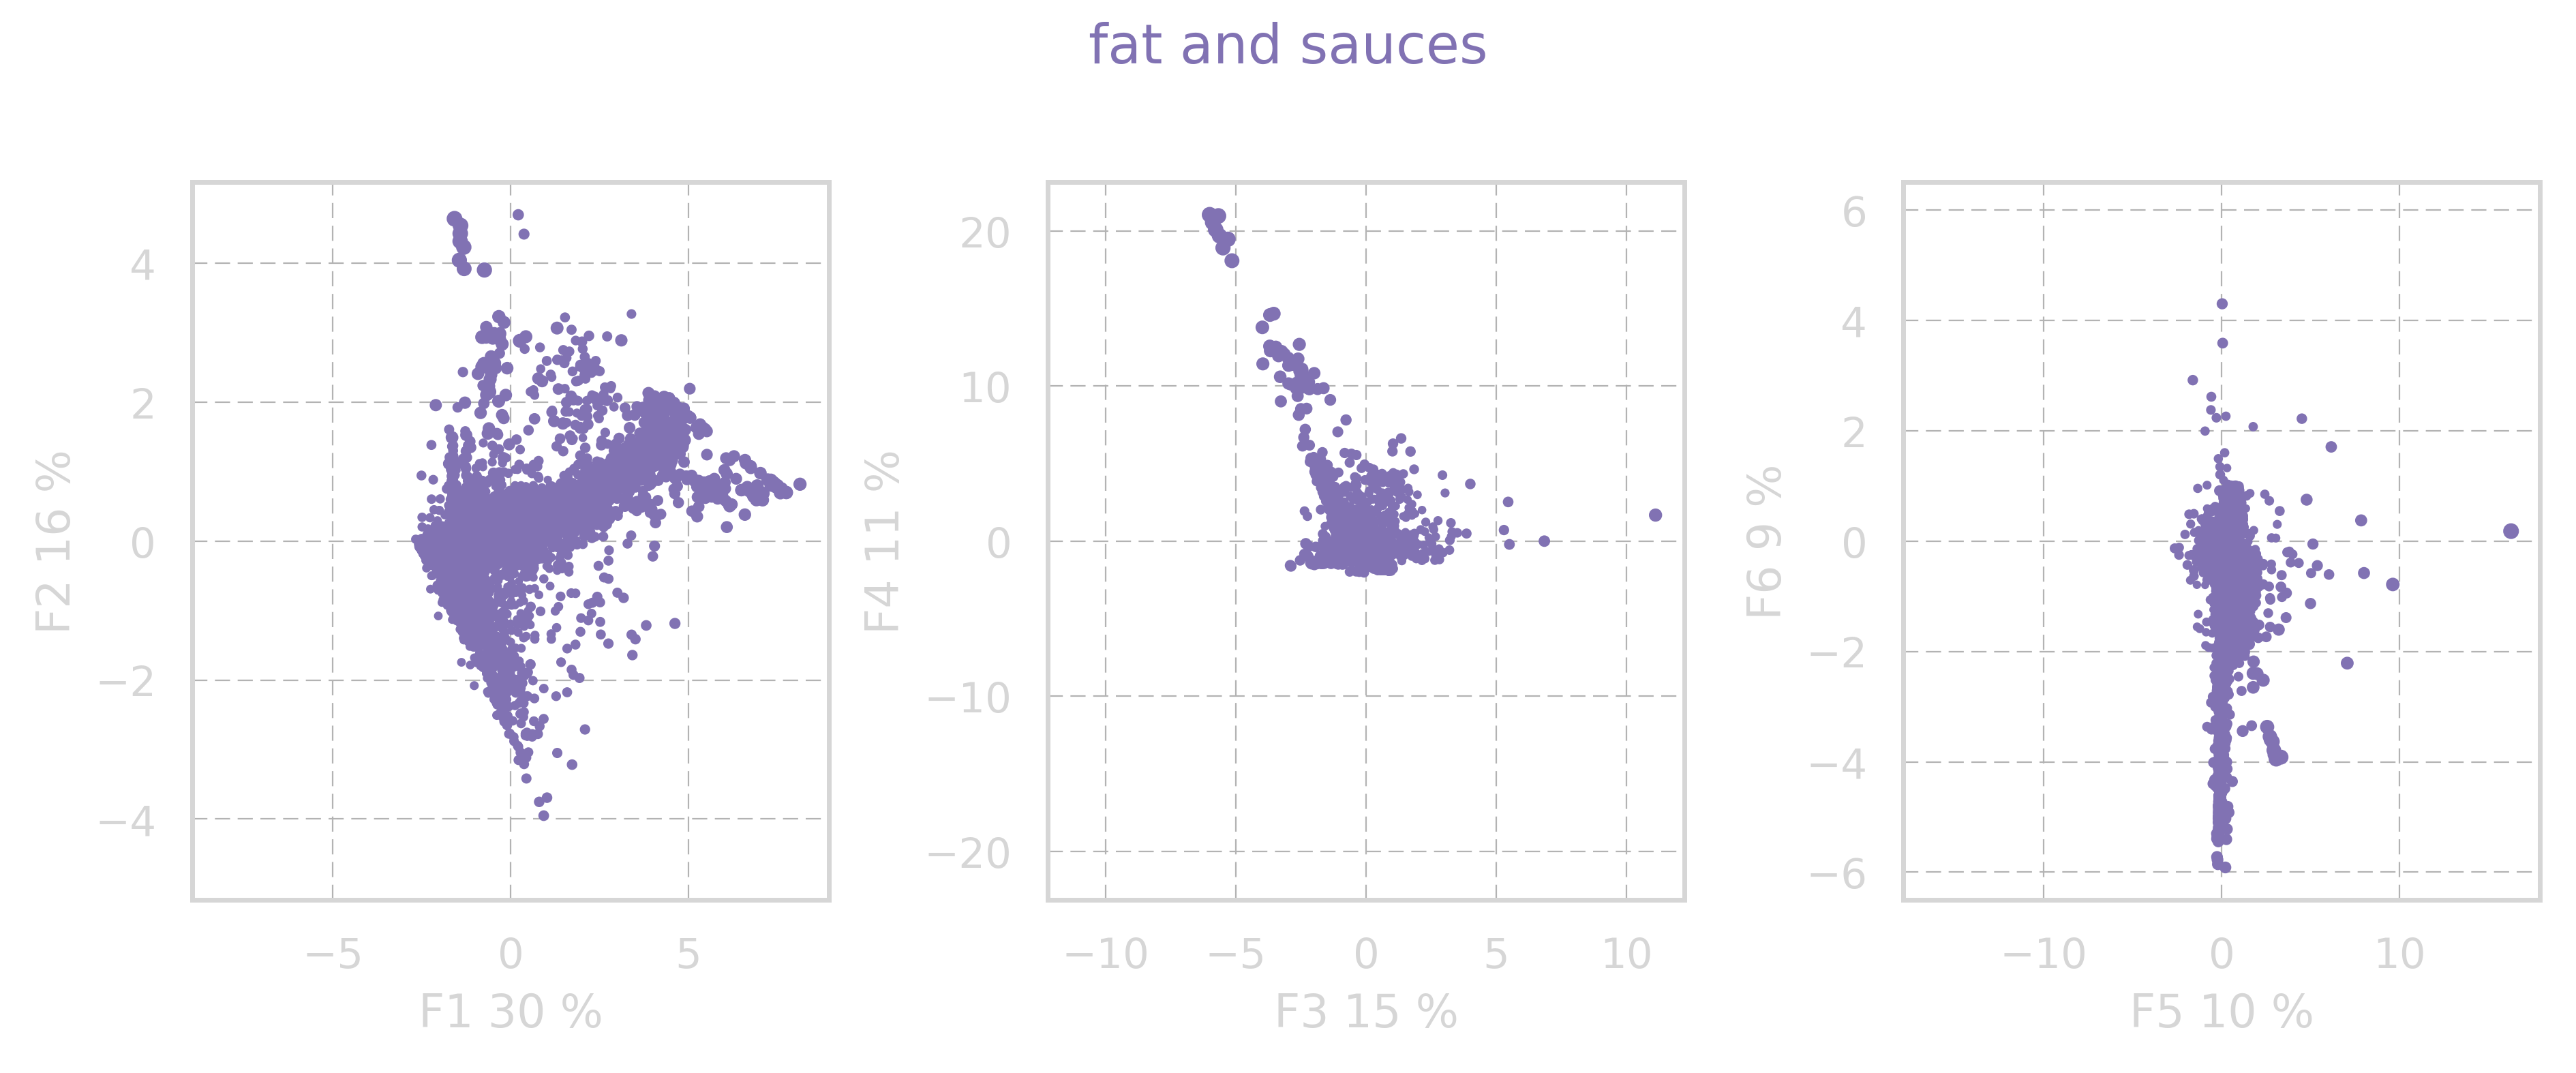
\includegraphics[width=80mm]{PCA/projection-fat-and-sauces.png}
			% 	} ;
			% }

		\end{scope}
	\end{tikzpicture}
\end{frame}


\subsection{Analyse des données en lien avec l'application}
\begin{frame}[t, label=pieCategories]
	\vspace{0mm}
	\begin{tikzpicture}
		\linespread{1}% <--- locally defined vertical line spacing in nodes
		\draw[clrBorders] (0,0) rectangle (\textwidth,\textheight) ;

		\node[anchor=west, text width=90mm] at (5mm,0.9\textheight) {Répartition pnns groups et nutriscore grade:} ;

		\only<2-4>{
			\node at (0.5\textwidth,0.5\textheight) {
				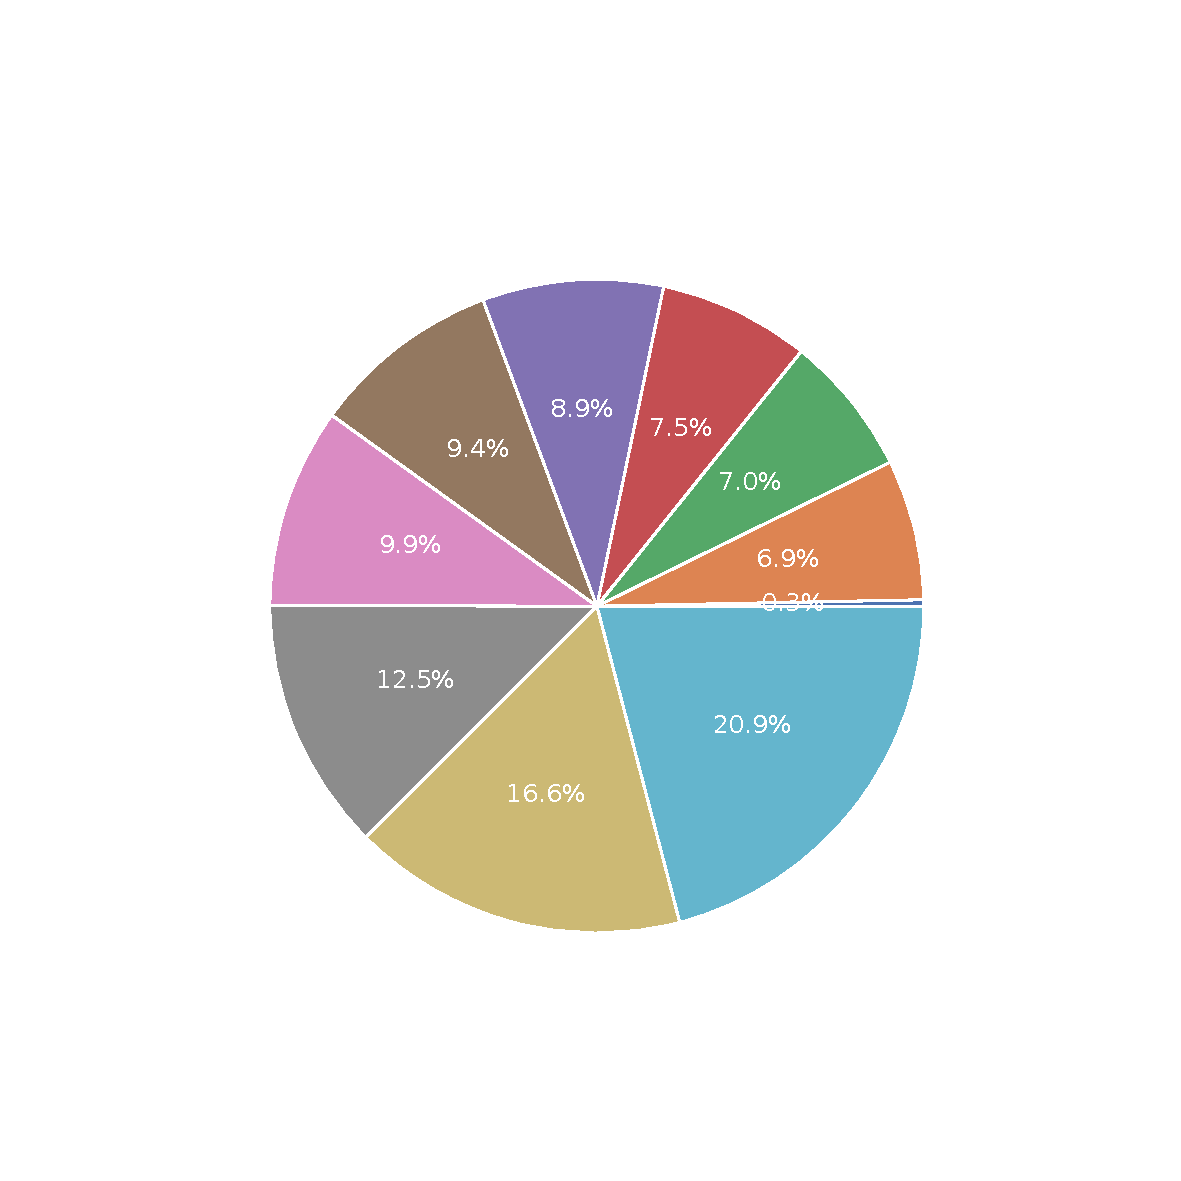
\includegraphics[width=85mm]{pie_pnns_groups_1.pdf}
			} ;
			\only<3>{
				\draw[myOrng, thick, rounded corners] (0.25\textwidth,21mm) rectangle (0.75\textwidth, 44.8mm) ;
				\node[myOrng] at (0.6\textwidth, 16mm) {Principaux éléments} ;
				}
				\only<4>{
					\draw[red, thick, rounded corners] (0.49\textwidth, 43mm) rectangle (0.75\textwidth,46mm) ;
					\node[red] at (0.85\textwidth, 40mm) {Très peu d'éléments} ;
			}
		}

		\only<5-6>{
			\node at (0.5\textwidth,0.5\textheight) {
				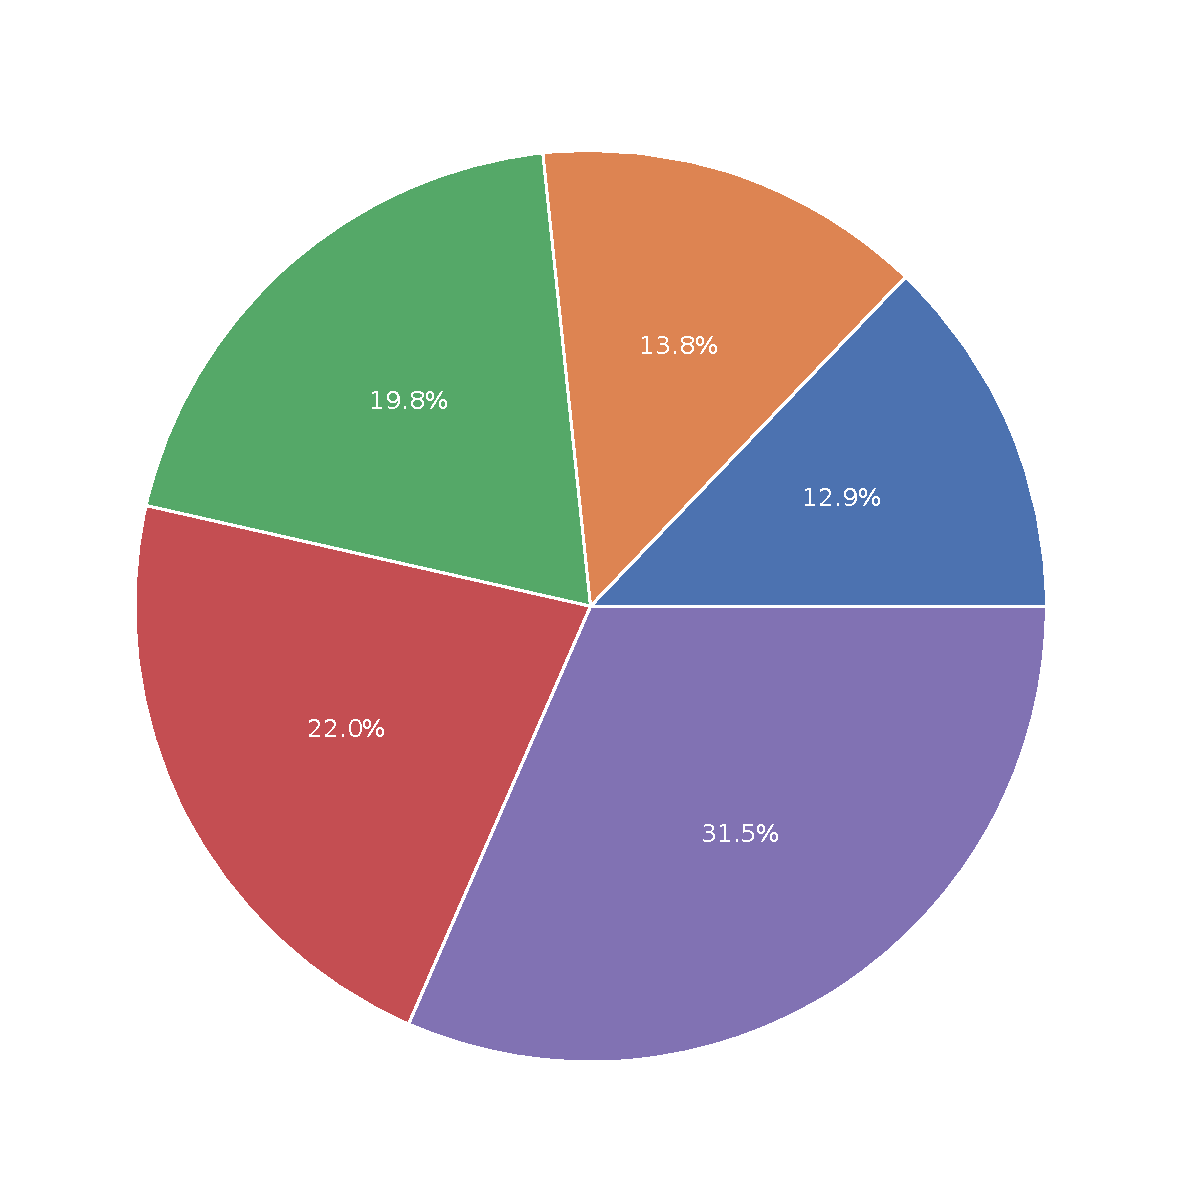
\includegraphics[width=60mm]{pie_nutriscore_grade.pdf}
			} ;
			\only<6>{
				\draw[myOrng, thick, rounded corners] (0.45\textwidth,43mm) rectangle (0.75\textwidth, 71mm) ;
				\node[myOrng] at (0.85\textwidth, 40mm) {Moindre proportion} ;
			}
		}

		% \node[text width=50mm] at (0.5\textwidth,0.8\textheight) {- Répartition inégales\\- boissones alcoolisées = peu d'entrées\\- + de C, D et E} ;

	\end{tikzpicture}
\end{frame}



\begin{frame}[t, label=ANOVA]
	\vspace{0mm}
	\begin{tikzpicture}
		\linespread{1}% <--- locally defined vertical line spacing in nodes
		\draw[clrBorders] (0,0) rectangle (\textwidth,\textheight) ;

		\node[anchor=west, text width=90mm] at (5mm,0.9\textheight) {Analyse de la corrélation entre le \alert{nutriscore grade} et la \alert{teneur en sel}:} ;

		\only<2>{
			\node at (0.5\textwidth,0.5\textheight) {
				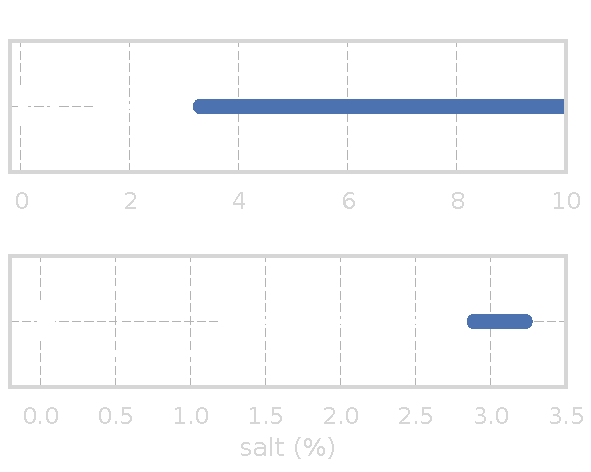
\includegraphics[width=60mm]{ANOVA/crop-outliers.pdf}
			} ;
		}

		\only<3->{
			\node at (0.25\textwidth,0.65\textheight) {
				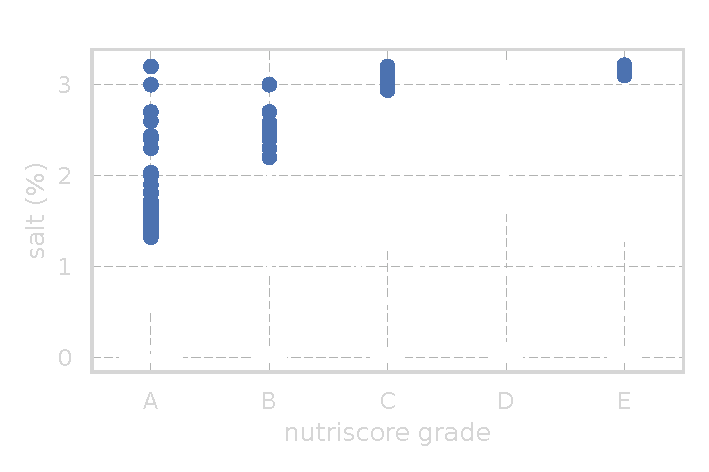
\includegraphics[width=50mm]{ANOVA/boxes.pdf}
			} ;
		}
		
		\visible<7-9>{
			\node[text centered] at (0.5\textwidth,0.2\textheight) {
				\begin{tabular}{ccccccc}
					\rowcolor{dfFirstRow}
					& $\sum y^2$ & DF & F & p-value & $\eta^2$ & $\omega^2$ \tabularnewline
					\rowcolor{dfEvenRow}
					nutriscore grade & 6456.376 & 4 & 3247.42 & 0.0 & 0.106 & 0.106 \tabularnewline
					\rowcolor{dfOddRow}
					Residual & 54512.732 & 109675 & & & &
				\end{tabular}
			} ;
		}
		\only<4-9>{
			\node[text centered] (A) at (0.25\textwidth,0.42\textheight)
				{Les groupes sont \alert{différents}} ;
		}

		\only<5->{
			\node at (0.72\textwidth,0.65\textheight) {
				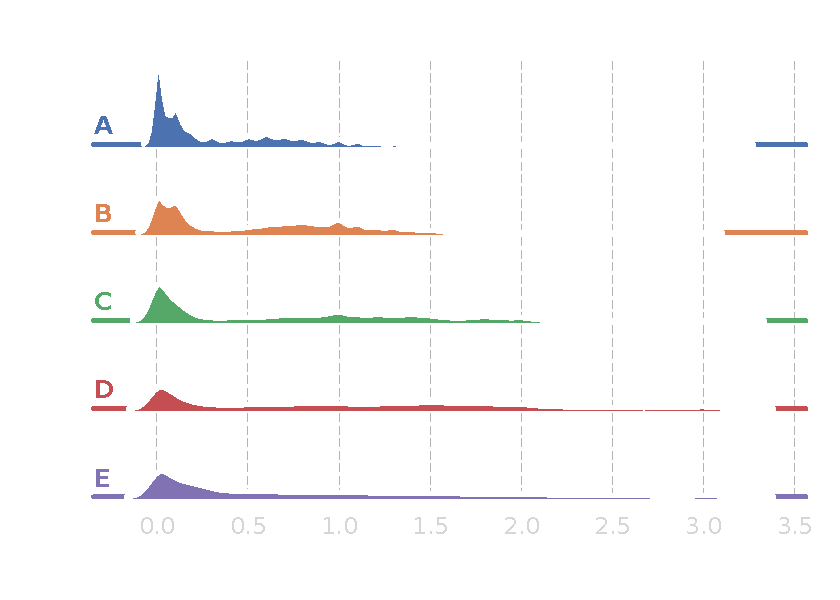
\includegraphics[width=55mm]{ANOVA/salt_grade_histo.pdf}
			} ;
		}

		\only<6-9>{
			\node[text width=20mm, text centered] at (0.9\textwidth,0.42\textheight) {Distributions \alert{multi-modales}} ;
			\node[text width=35mm, text centered] (B) at (0.57\textwidth,0.4\textheight) {Les moyennes sont\\\alert{faiblement} corrélées\\au "grade"} ;
		}

		\only<8-9>{
			\begin{scope}[xshift=57.25mm, yshift=16.5mm]
				\draw[myOrng, thick, rounded corners] (0,0) rectangle (26mm,7mm) ;
				\draw[myarrow] (A) to [out=-90, in=130] (0mm, 7mm) ;
			\end{scope}
		}

		\only<9>{
			\begin{scope}[xshift=84.25mm, yshift=16.5mm]
				\draw[myOrng, thick, rounded corners] (0,0) rectangle (21mm,7mm) ;
				\draw[myarrow] (B) to [out=-40, in=110] (3mm, 7mm) ;
			\end{scope}
		}

		\only<10->{
			\node at (0.5\textwidth,0.25\textheight) {
				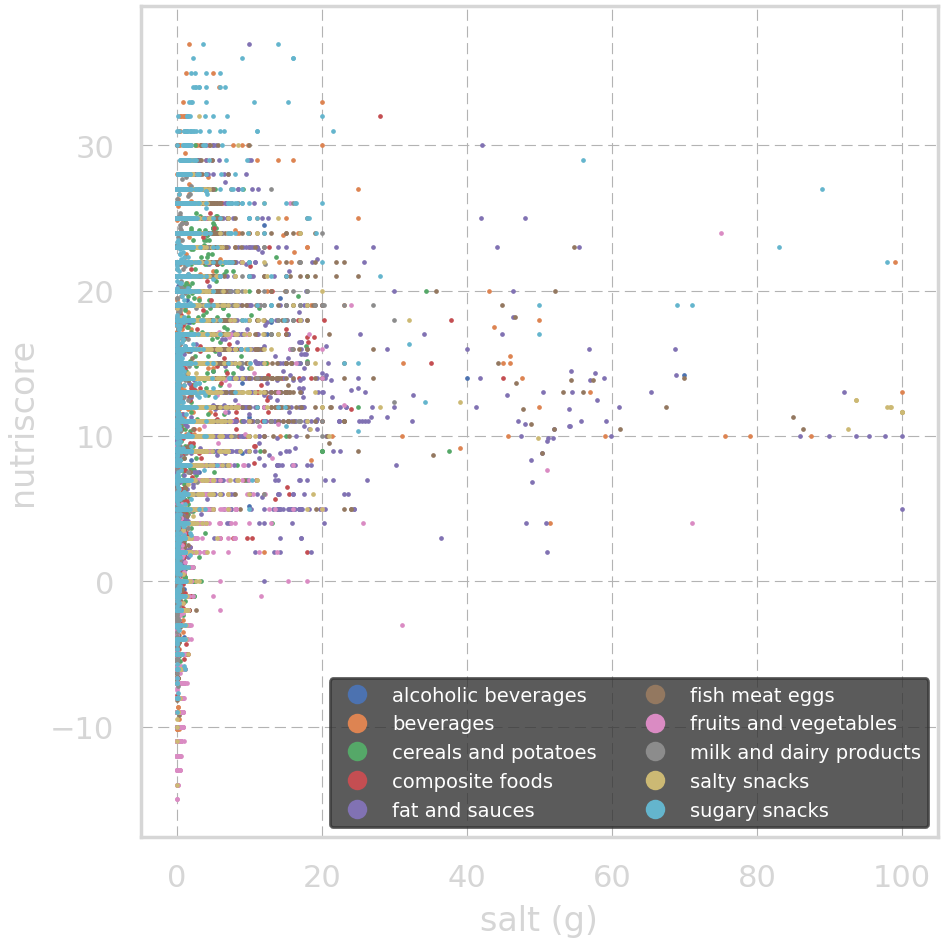
\includegraphics[width=40mm]{scatter/salt.png}
			} ;
		}

		\only<11->{
			\node[myOrng, box_style00, very thick, text width=20mm] (CCL) at (0.85\textwidth,0.2\textheight) {Aucune corrélation apparente} ;
			\draw[myarrow] (0.69\textwidth, 0.2\textheight) -- (CCL) ;
		}

	\end{tikzpicture}
\end{frame}


\begin{frame}[t, label=sugars]
	\vspace{0mm}
	\begin{tikzpicture}
		\linespread{1}% <--- locally defined vertical line spacing in nodes
		\draw[clrBorders] (0,0) rectangle (\textwidth,\textheight) ;

		\node[anchor=west, text width=90mm] at (5mm,0.9\textheight) {Analyse de la relation \alert{nutriscore} et la \alert{teneur en sucres}:} ;

		\only<2->{
			\node at (0.5\textwidth,0.5\textheight) {
				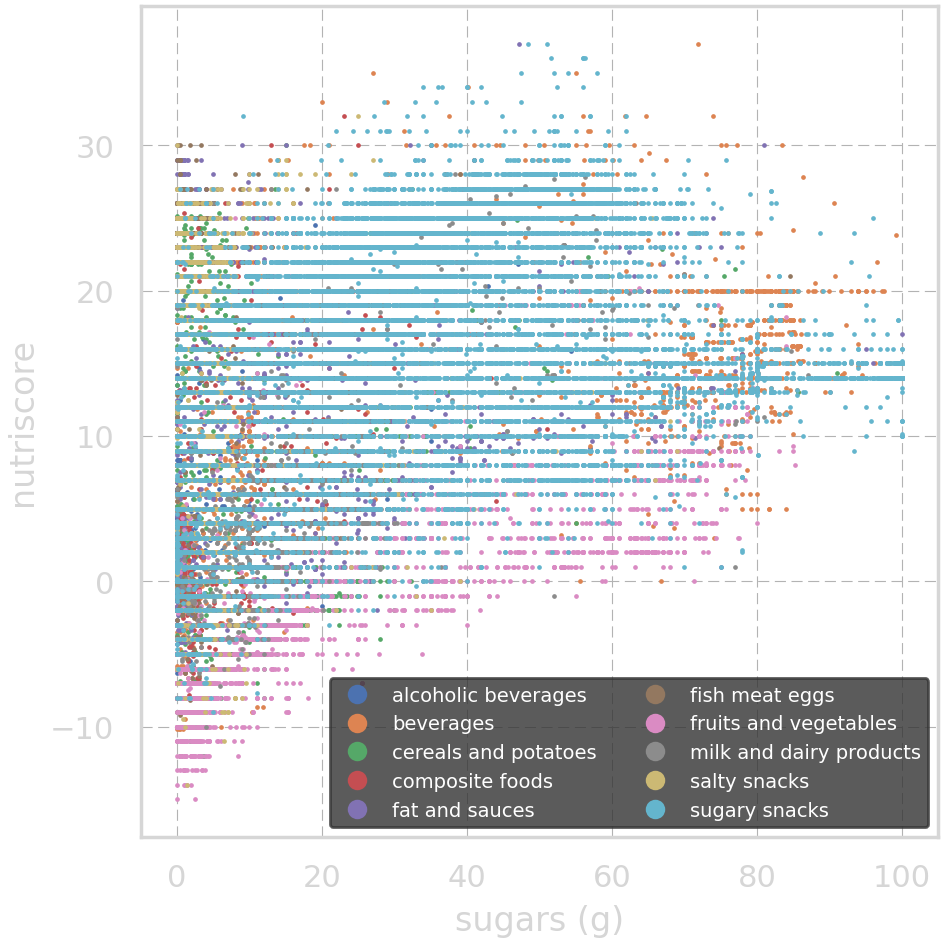
\includegraphics[width=60mm]{scatter/sugars.png}
			} ;
		}

		\only<3->{
			\begin{scope}[xshift=0.5\textwidth, yshift=0.58\textheight]
				\begin{scope}[rotate=37]
					\draw[myOrng, very thick] (0,0) circle [x radius=25mm, y radius = 14 mm] ;
				\end{scope}
			\end{scope}
			\node at (0.5\textwidth,10mm) {Une \alert{corrélation} est \alert{visible}, mais d'\alert{autres variables} influencent aussi le nutriscore } ;
		}
		% \only<2>{
		% 	\node at (0.5\textwidth,0.5\textheight) {
		% 		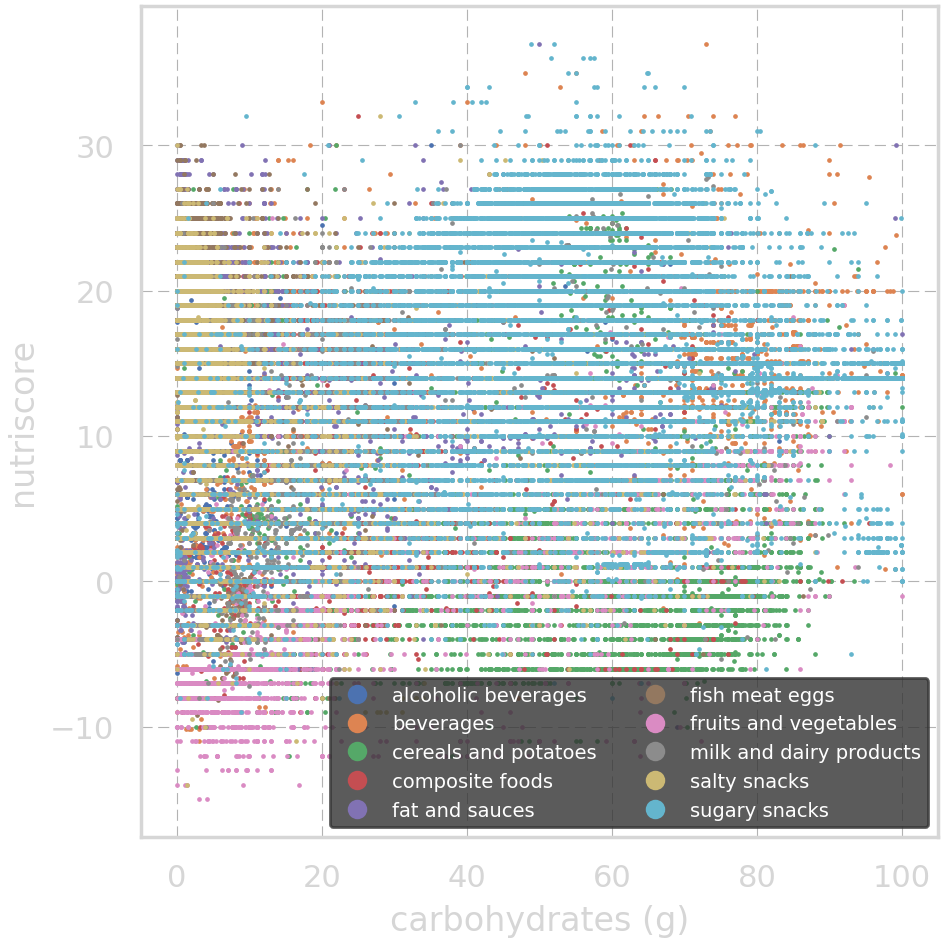
\includegraphics[width=60mm]{scatter/carbohydrates.png}
		% 	} ;
		% }


		% \only<3>{
		% 	\node at (0.5\textwidth,0.5\textheight) {
		% 		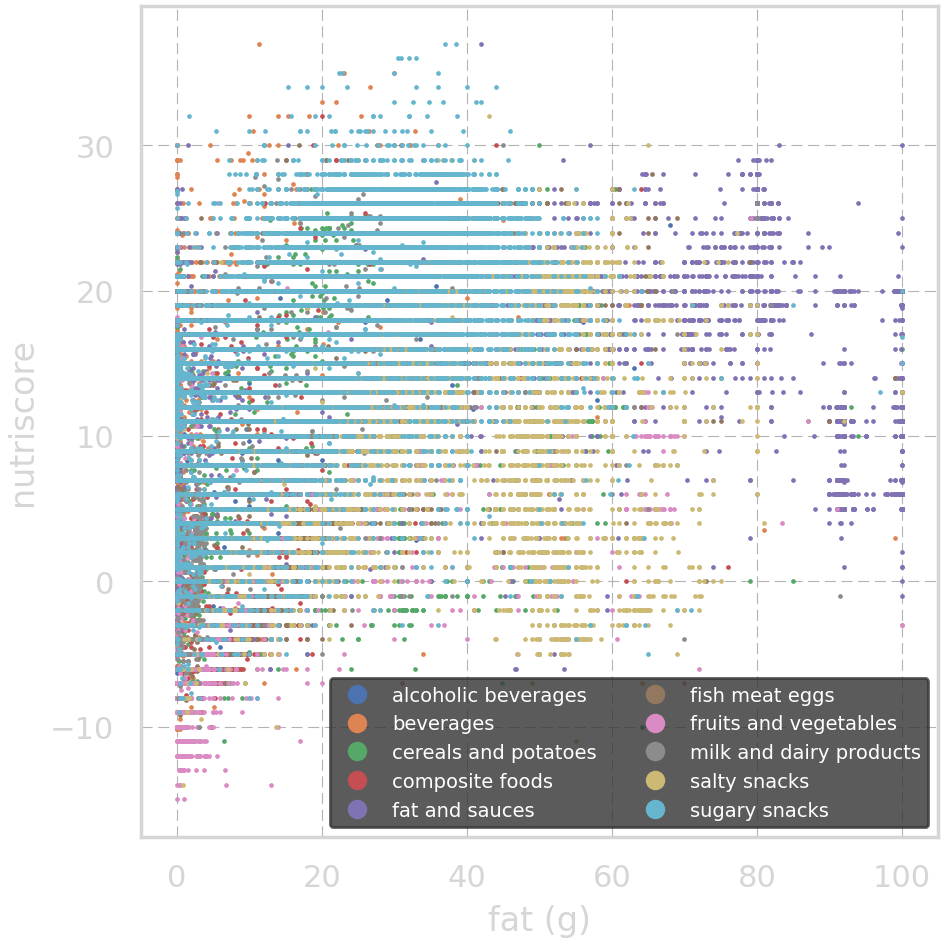
\includegraphics[width=60mm]{scatter/fat.png}
		% 	} ;
		% }

		% \only<4>{
		% 	\node at (0.5\textwidth,0.5\textheight) {
		% 		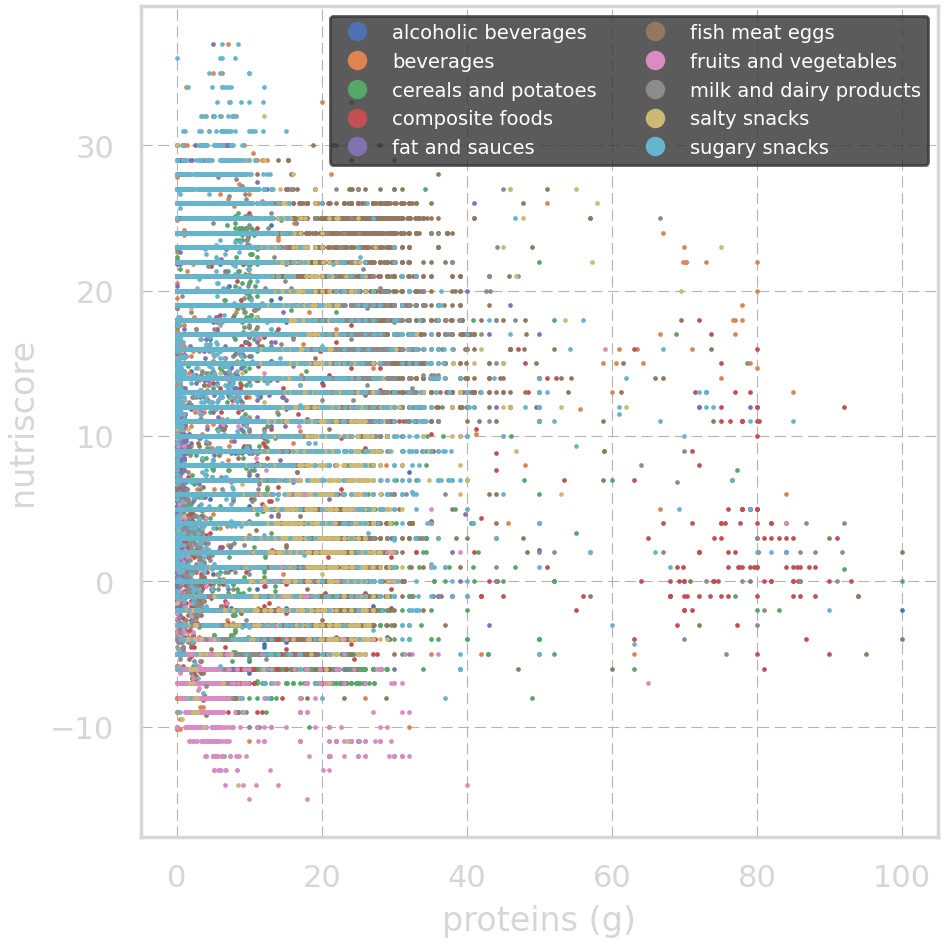
\includegraphics[width=60mm]{scatter/proteins.png}
		% 	} ;
		% }


		

	\end{tikzpicture}
\end{frame}


\begin{frame}[t, label=ingredientsTexte]
	\vspace{0mm}
	\begin{tikzpicture}
		\linespread{1}% <--- locally defined vertical line spacing in nodes
		\draw[clrBorders] (0,0) rectangle (\textwidth,\textheight) ;

		\node[anchor=west, text width=90mm] at (5mm,0.9\textheight) {Peut-on calculer l'indice glycémique ?} ;

		\only<2->{
			\node at (0.27\textwidth,0.78\textheight) {Exemple de listes d'ingrédients:} ;
			\node[text width=50mm] at (0.3\textwidth,0.5\textheight) {
				\tiny
				$\bullet$ lait entier (99\%); poudre de lait (1\%), ferments lactiques, présure.
				\\\vspace{2mm}
				$\bullet$ jus d'orange 40\% - jus de pomme 40\% - jus d'ananas 9\% - purée de banane - jus de raisin blanc - jus de pamplemousse - purée d'abricot - purée de pêche.
				\\\vspace{2mm}
				$\bullet$ 1 boite  de garniture: tomates fraiches (51\%), eau, oignons frais, huile d'olive vierge extra, huile de colza, sel, persil, concentré de tomate, jus concentré de citron, menthe, épaississants: farine de graines de caroube et gomme guar, arômes. 1 coupelle de semoule de blé dur précuite à la vapeur.
				\\\vspace{2mm}
				$\bullet$ farine de blé, sucre, beurre 12\% (lait), sirop de sucre inverti, poudres à lever: carbonates de sodium, diphosphates, lactosérum en poudre lait), lat entier en poudre, sel, émulsifiant: lécithine de soja; acidifiant : acide citrique; arôme (oeufs entiers en poudre).
				\\\vspace{2mm}
				$\bullet$ palette de porc avec os 90 \%, eau, sel, dextrose, conservateur : nitrite de sodium.
				\\
			} ;
		}

		\only<3->{
			\node[myOrng, box_style00, very thick, text width=40mm] at (0.75\textwidth,0.7\textheight) {Non, car les \% sont\\assez peu renseignés} ;
		}

		\only<4>{
			\node at (0.75\textwidth,0.4\textheight) {
				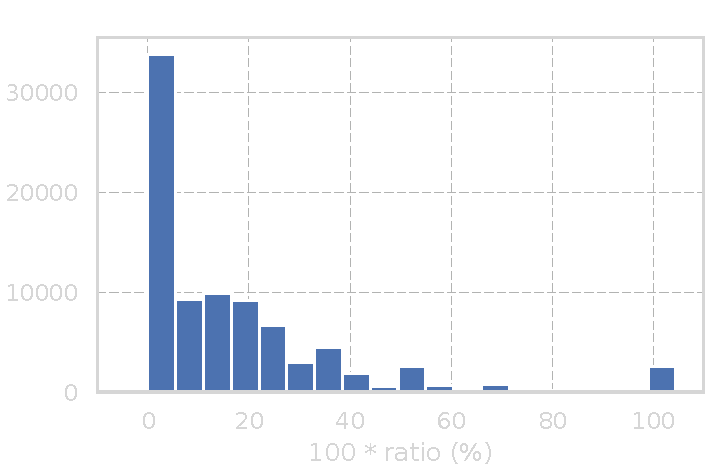
\includegraphics[width=40mm]{ratio_percent_sep.pdf}
			} ;
		}


	\end{tikzpicture}
\end{frame}



\section{CONCLUSIONS}

\begin{frame}[t, label=CCL]
	\vspace{0mm}
	\begin{tikzpicture}
		\linespread{1}% <--- locally defined vertical line spacing in nodes
		\draw[clrBorders] (0,0) rectangle (\textwidth,\textheight) ;

		\node[anchor=west, text width=90mm] at (5mm,0.9\textheight) {Résultats de la faisabilité des applications:} ;

		\visible<2->{
			\node[text centered] at (0.25\textwidth,0.8\textheight) {Données récupérables:} ;
		}
		\visible<4->{
			\node[ text centered] at (0.75\textwidth,0.8\textheight) {Applications:} ;
		}

		\visible<3->{
		\begin{scope}[xshift=0.25\textwidth, yshift=1.5mm]
			\node[box_style00, minimum height=8mm, text width=35mm] at (0,0.65\textheight) {Teneur en sel} ;
			\node[box_style00, minimum height=8mm, text width=35mm] at (0,0.55\textheight) {Charge calorique} ;
			\node[box_style00, minimum height=8mm, text width=35mm] at (0,0.45\textheight) {Présence d'ingrédients\\dont allergènes} ;
			\node[box_style00, minimum height=8mm, text width=35mm] at (0,0.315\textheight) {Pourcentage de macro-nutriments\\notamment graisses et sucres} ;
		\end{scope}
		}

		\begin{scope}[xshift=0.75\textwidth, yshift=3mm]
			\visible<5->{
				\node[green, box_style00, minimum height=8mm, text width=35mm] at (0,0.65\textheight) {Régime pauvre en sel} ;
				\node[green, box_style00, minimum height=8mm, text width=35mm] at (0,0.55\textheight) {Gestion de poids/IMC} ;
				\node[green, box_style00, minimum height=8mm, text width=35mm] at (0,0.45\textheight) {Régime sans/avec ...} ;
			}
			\visible<6->{
			\node[red, box_style00, minimum height=8mm, text width=35mm] at (0,0.35\textheight) {Gestion de l'indice glycémique} ;
			\node[red, box_style00, minimum height=8mm, text width=35mm] at (0,0.25\textheight) {Gestion équilibre acido-basique} ;
			}
		\end{scope}
		
		\visible<7->{
			\node[text width=95mm, text centered] at (0.5\textwidth,0.12\textheight) {Se rapprocher de \alert{spécialistes} du domaine\\est \alert{nécessaire} pour apporter une\\meilleure \alert{connaissance métier}\\(identifier/valider les contraintes\\alimentaires liées aux états de santé)} ;
		}
	\end{tikzpicture}
\end{frame}


\begin{frame}[t, label=CCL2]
	\vspace{0mm}
	\begin{tikzpicture}
		\linespread{1}% <--- locally defined vertical line spacing in nodes
		\draw[clrBorders] (0,0) rectangle (\textwidth,\textheight) ;

		\node[anchor=west, text width=90mm] at (5mm,0.9\textheight) {Pistes d'améliorations des traitements:} ;

		\visible<2->{
			\node[box_style00, text width=40mm] (A) at (0.25\textwidth,0.6\textheight) {Améliorer la \alert{gestion} des \alert{NaN}} ;
		}
		\visible<3->{
			\begin{scope}[xshift=0.15\textwidth]
				\node[box_style00, text width=18mm] (B) at (0,0.4\textheight) {Déterminer le \alert{pnns groups} à partir de la liste des ingrédients} ;
				\draw[myarrow] (0,52.8mm) -- (B) ;
			\end{scope}
		}

		\visible<4->{
			\begin{scope}[xshift=0.35\textwidth]
				\node[box_style00, text width=18mm] (B2) at (0,0.4\textheight) {Remplacement des \alert{NaN éparses}} ;
				\draw[myarrow] (0,52.8mm) -- (B2) ;
			\end{scope}
		}
		
		\visible<5->{
			\node[box_style00, text width=40mm] (C) at (0.75\textwidth,0.6\textheight) {Mettre en place des \alert{moteurs} de \alert{recommandation}} ;
		}

		\visible<6->{
			\begin{scope}[xshift=0.65\textwidth]
				\node[box_style00, text width=18mm] (D) at (0,0.4\textheight) {Basé sur le \alert{contenu}} ;
				\draw[myarrow] (0,51.4mm) -- (D) ;
			\end{scope}
			
			\begin{scope}[xshift=0.85\textwidth]
				\node[box_style00, text width=18mm] (E) at (0,0.4\textheight) {\alert{Filtrage collaboratif}} ;
				\draw[myarrow] (0,51.4mm) -- (E) ;
			\end{scope}
		}
		
	\end{tikzpicture}
\end{frame}

\begin{frame}[t, label=Merci]
	\vspace{0mm}
	\begin{tikzpicture}
		\linespread{1}% <--- locally defined vertical line spacing in nodes
		\draw[clrBorders] (0,0) rectangle (\textwidth,\textheight) ;

		\node at (0.5\textwidth,0.5\textheight) {\huge \alert{Merci} pour votre \alert{attention}.} ;

	\end{tikzpicture}
\end{frame}

\appendix


\section{knn}

\begin{frame}[t, label=knn]
	\vspace{0mm}
	\begin{tikzpicture}
		\linespread{1}% <--- locally defined vertical line spacing in nodes
		\draw[clrBorders] (0,0) rectangle (\textwidth,\textheight) ;

		\node[anchor=west] at (5mm,0.9\textheight) {{Principe:}} ;

		\begin{scope}[xshift=0.15\textwidth]
			\node[box_style00, text width=20mm] (A)
				at (0,0.75\textheight) {Données \alert{connues}} ;
				% at (0,0.75\textheight) {Calcul de la \alert{distance euclidienne} entre une \alert{entrée cible} et les \alert{entrée à sortie connue}} ;


			\visible<2->{
				\node[box_style00, text width=20mm] (B)
					at (0,0.4\textheight) {Entrée à \alert{sortie inconnue}} ;
			}

			\visible<3->{
				\node[box_style00, text width=20mm] (C)
					at (0,0.575\textheight) {Calcul des \alert{distances euclidiennes}} ;
				\draw[myarrow] (A) -- (C) ;
				\draw[myarrow] (B) -- (C) ;
			}
		\end{scope}

		\visible<4->{
			\node[box_style00, text width=20mm, anchor=center] (D)
				at (0.45\textwidth,0.75\textheight) {Sélection des \alert{k plus proches}} ;
			\draw[myarrow] (C) -| (D) ;
		}

		\visible<5->{
			\node[box_style00, text width=30mm, anchor=center] (E)
				at (0.8\textwidth,0.75\textheight) {Calcul de la \alert{valeur moyenne} pour les k éléments} ;
			\draw[myarrow] (D) -- (E) ;
		}

		\visible<6->{
		\node at (0.62\textwidth,0.35\textheight) {
			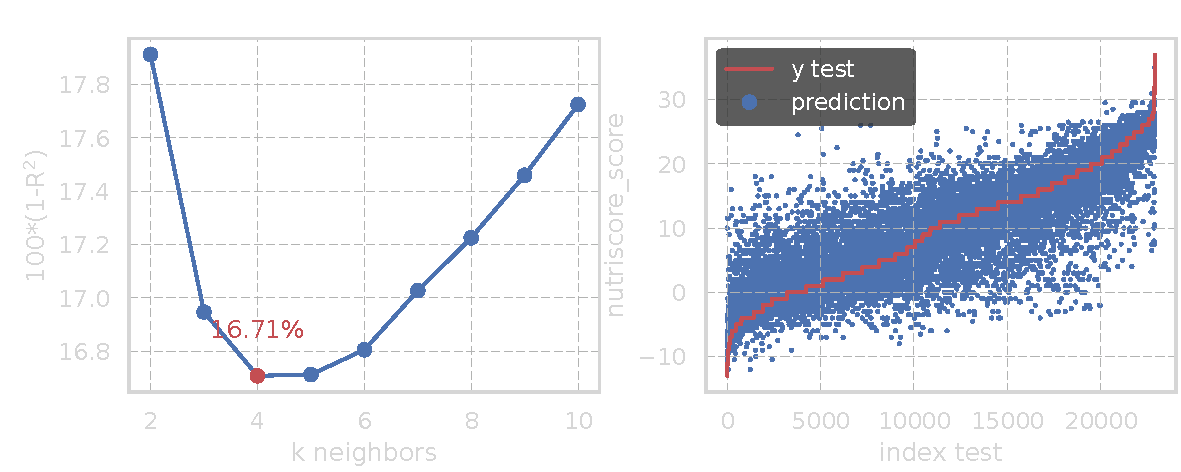
\includegraphics[width=78mm]{knn/0.pdf}
		} ;
		}

		\visible<7->{
			\draw[myOrng, thick] (48.5mm,25mm) circle (4mm) ;
			\node at (0.5\textwidth,0.1\textheight) {Avec les \alert{données brutes}, \alert{17\%} d'erreur $\rightarrow$ nécessité d'optimiser} ;
		}

	\end{tikzpicture}
\end{frame}

\begin{frame}[t, label=knnCorrelVars]
	\vspace{0mm}
	\begin{tikzpicture}
		\linespread{1}% <--- locally defined vertical line spacing in nodes
		\draw[clrBorders] (0,0) rectangle (\textwidth,\textheight) ;

		\node[anchor=west] at (5mm,0.9\textheight) {{Analyse de la \alert{corrélation} entre les variables:}} ;

		\visible<2->{
			\begin{scope}[xshift=0.45\textwidth, yshift=0.72\textwidth]
				\node[text centered] at (-12mm,0) {\small données originales} ;
				\node[text centered] at (17mm,0) {\small x'=x-y} ;
			\end{scope}
			\begin{scope}[yshift=0.7\textheight]
				\node at (0.45\textwidth,0) {
					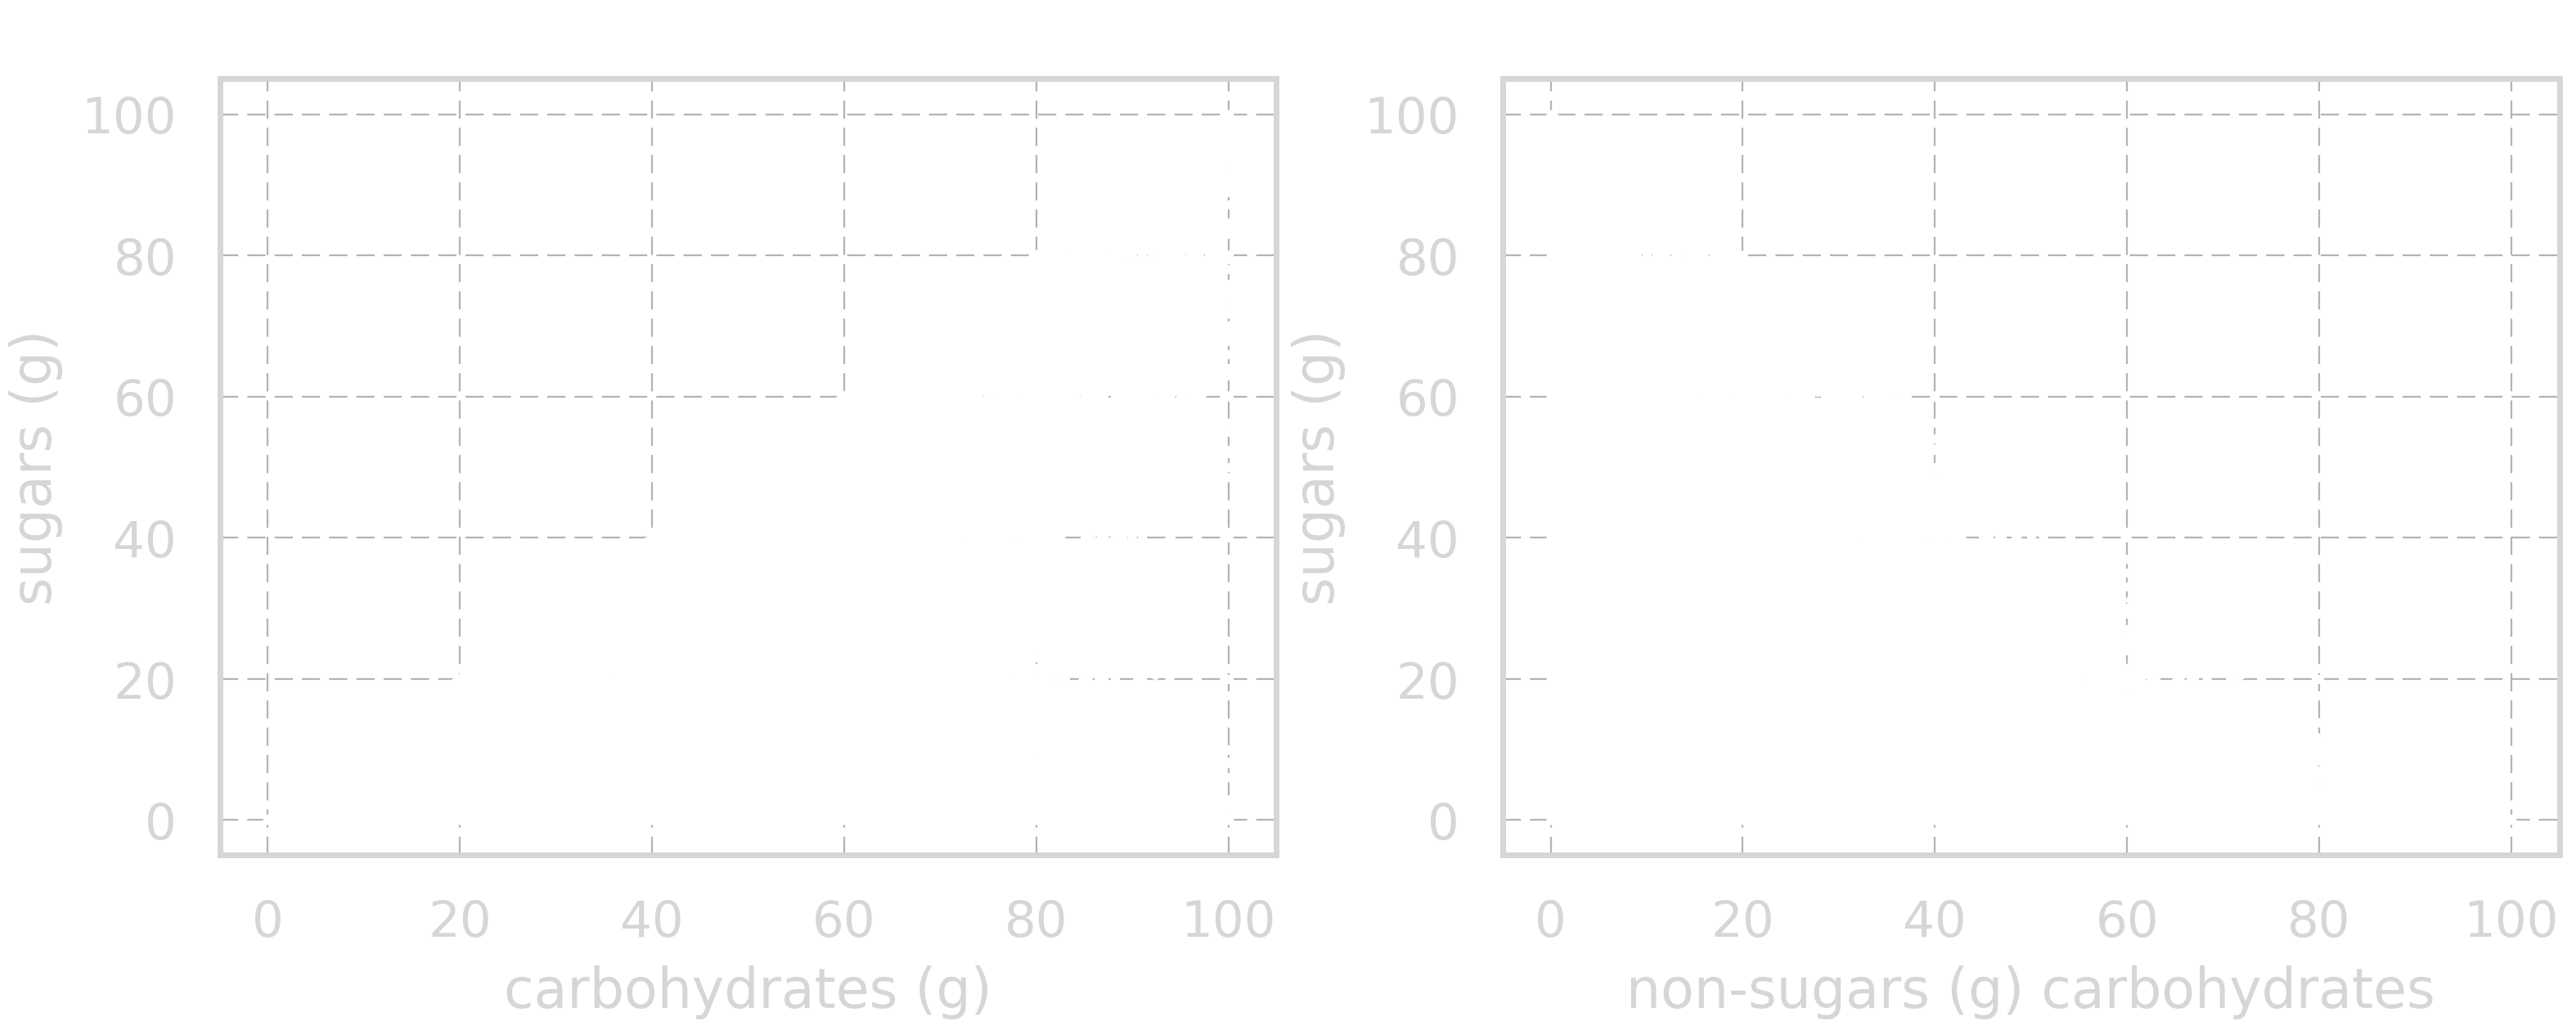
\includegraphics[width=60mm]{knn/correl_carbohydrates_100g.png}
				} ;
				\node[text centered, text width=11mm, font=\fontsize{7}{7}\selectfont] at (7mm,0) {carbohydrates\\/ sugars} ;
				\visible<3->{
					\node at (0.86\textwidth,0) {Décorrélation \alert{OK}} ;
				}
			\end{scope}
			}
		\visible<4->{
			\begin{scope}[yshift=0.42\textheight]
				\node at (0.45\textwidth,0) {
					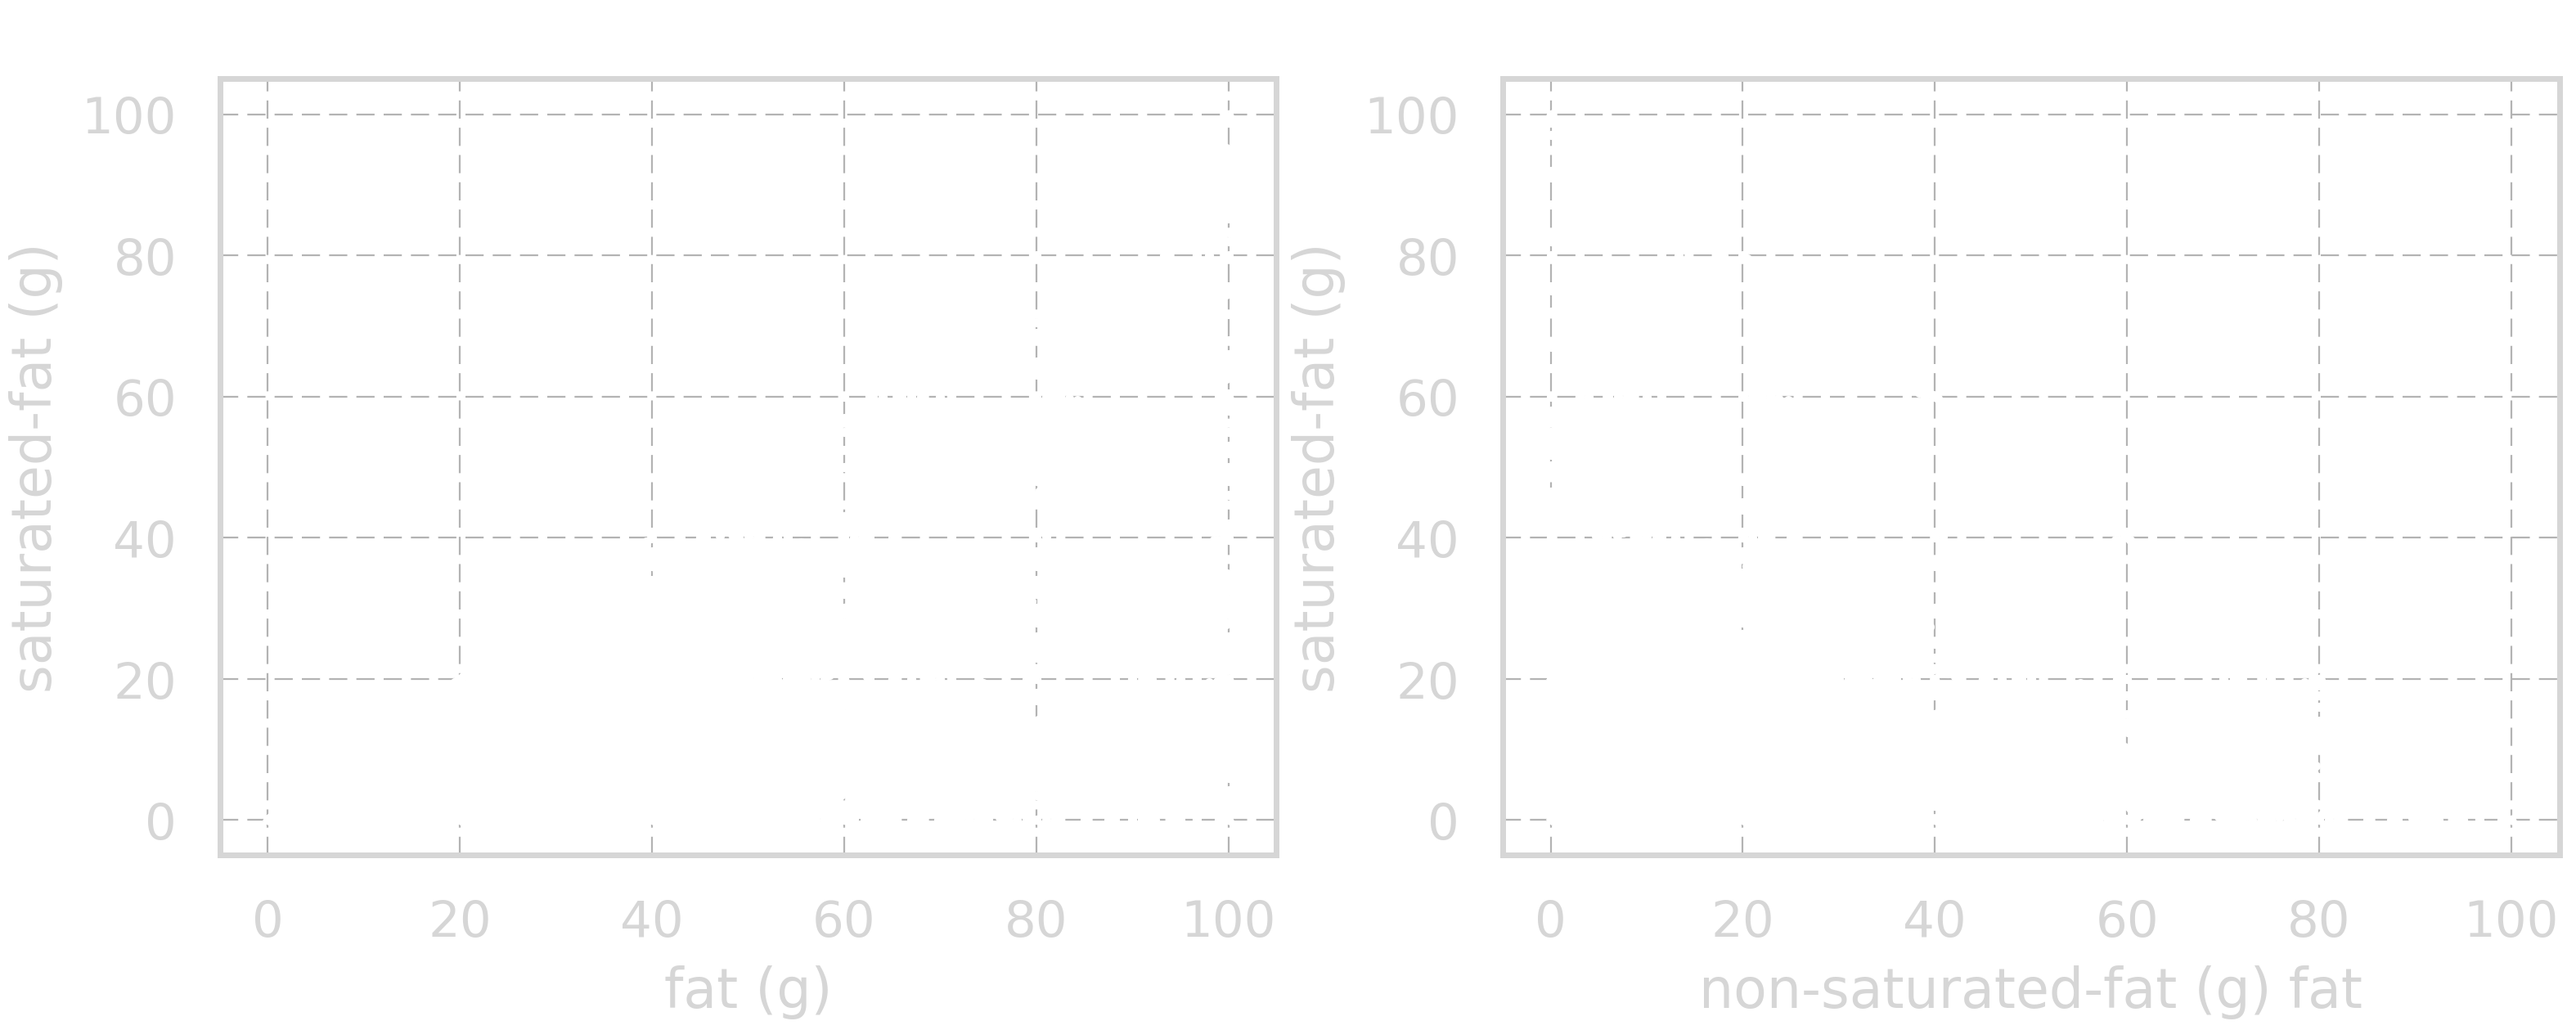
\includegraphics[width=60mm]{knn/correl_fat_100g.png}
				} ;
				\node[text centered, text width=11mm, font=\fontsize{7}{7}\selectfont] at (8mm,0) {fat /\\saturated-fat} ;
				\visible<5->{
					\node[text width=25mm, text centered] at (0.86\textwidth,0) {Décorrélation\\\alert{partielle}} ;
				}
			\end{scope}
		}
		\visible<6->{
			\begin{scope}[yshift=0.14\textheight]
				\node at (0.45\textwidth,0) {
					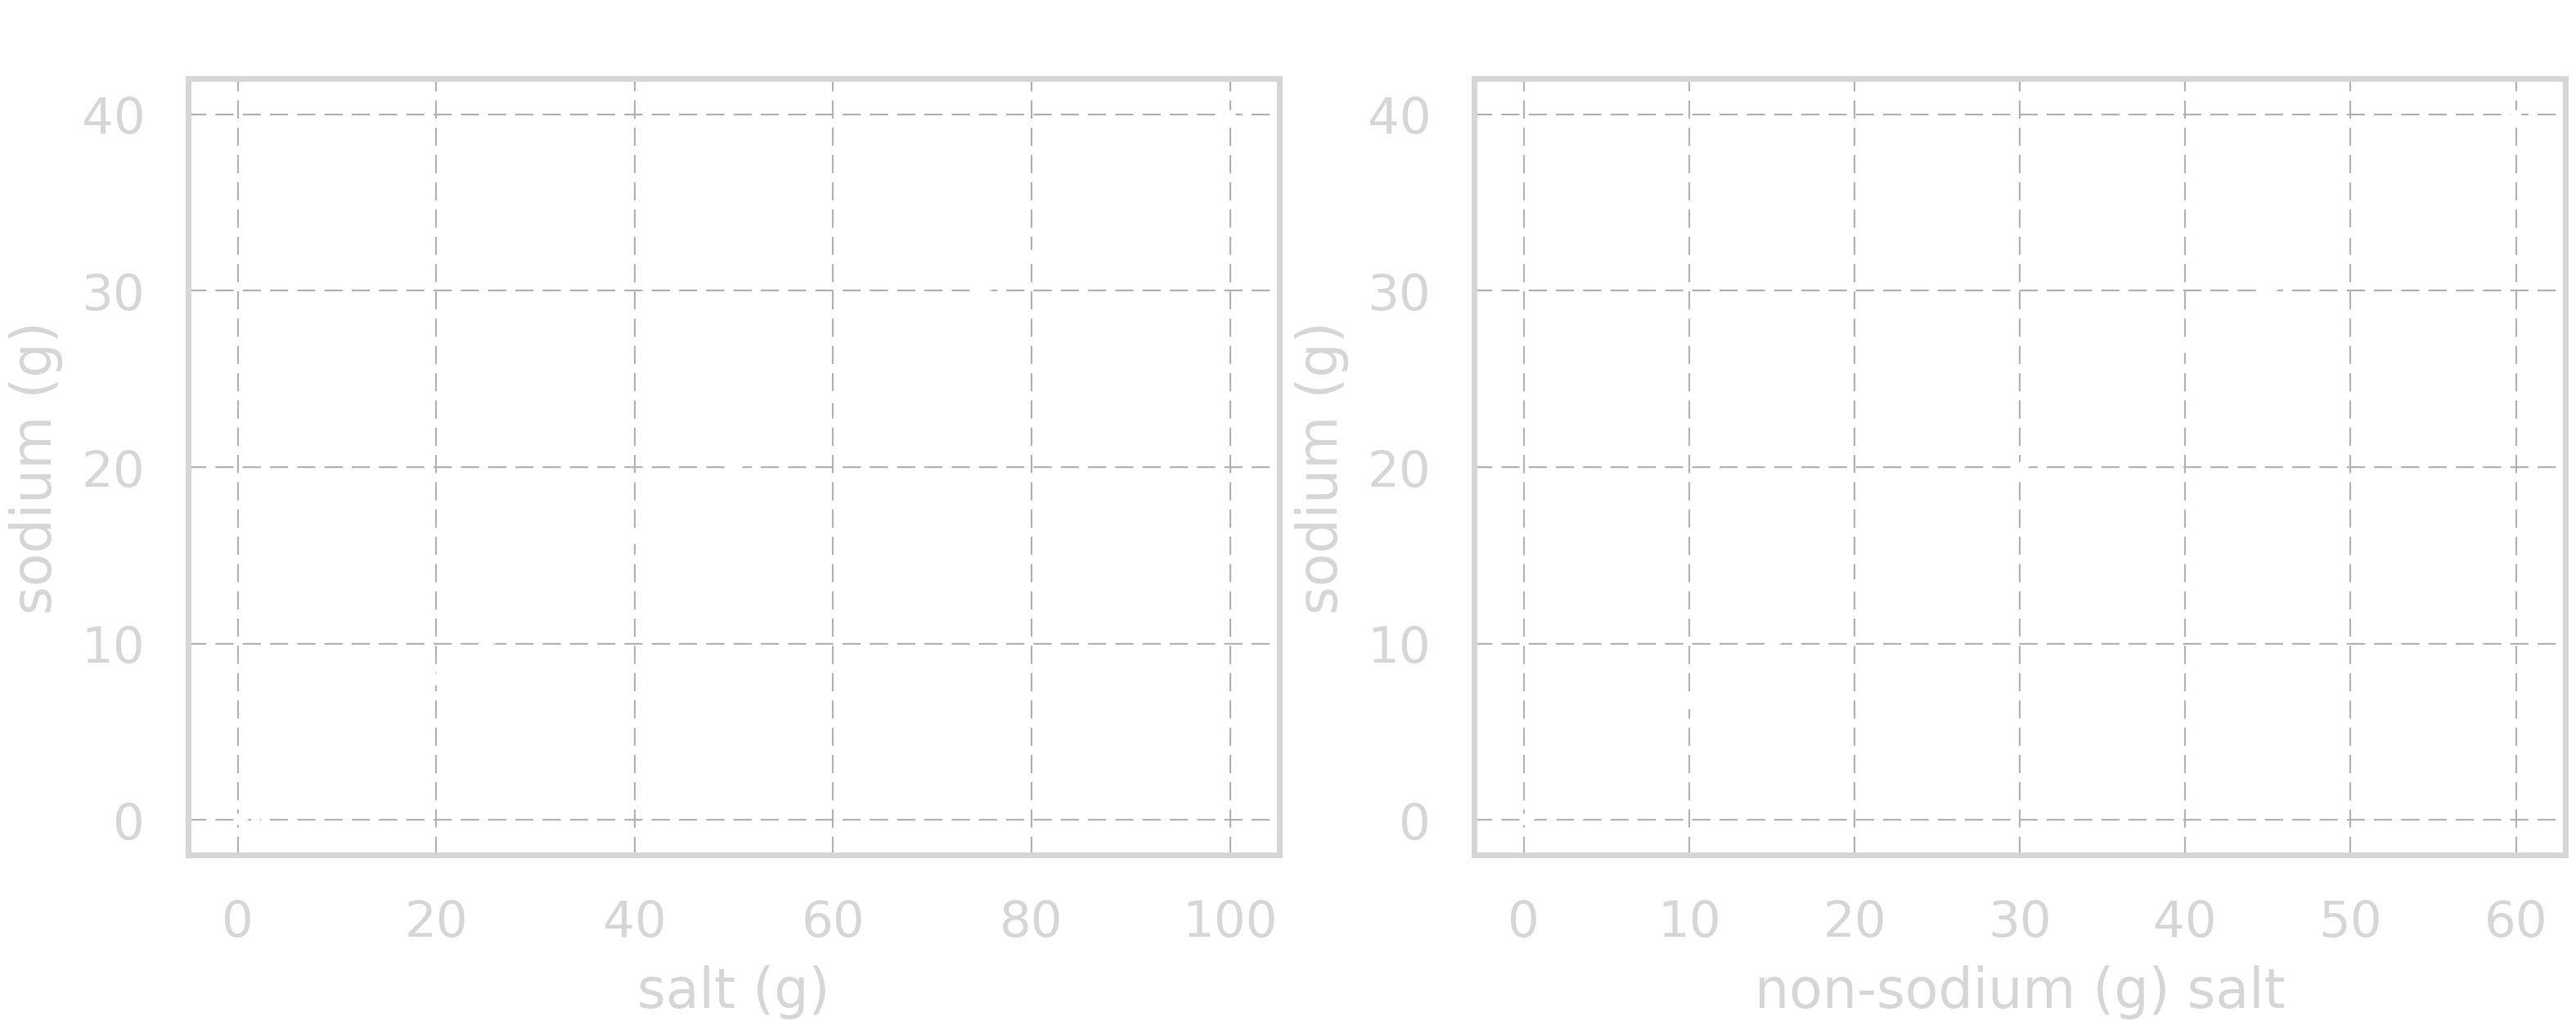
\includegraphics[width=60mm]{knn/correl_salt_100g.png}
				} ;
				\node[text centered, text width=11mm, font=\fontsize{7}{7}\selectfont] at (8mm,0) {sodium /\\fat} ;
				\visible<7->{
					\node[text width=25mm, text centered] at (0.86\textwidth,0) {Décorrélation\\\alert{nulle}\\$\rightarrow$ \alert{suppression} d'une variable} ;
				}
			\end{scope}

		}

	\end{tikzpicture}
\end{frame}

\begin{frame}[t, label=knnUpgraded]
	\vspace{0mm}
	\begin{tikzpicture}
		\linespread{1}% <--- locally defined vertical line spacing in nodes
		\draw[clrBorders] (0,0) rectangle (\textwidth,\textheight) ;

		\node[anchor=west] at (5mm,0.9\textheight) {Prédiction en utilisant la \alert{base améliorée}:} ;

		\only<2-3>{
			\node at (0.48\textwidth,0.55\textheight) {
				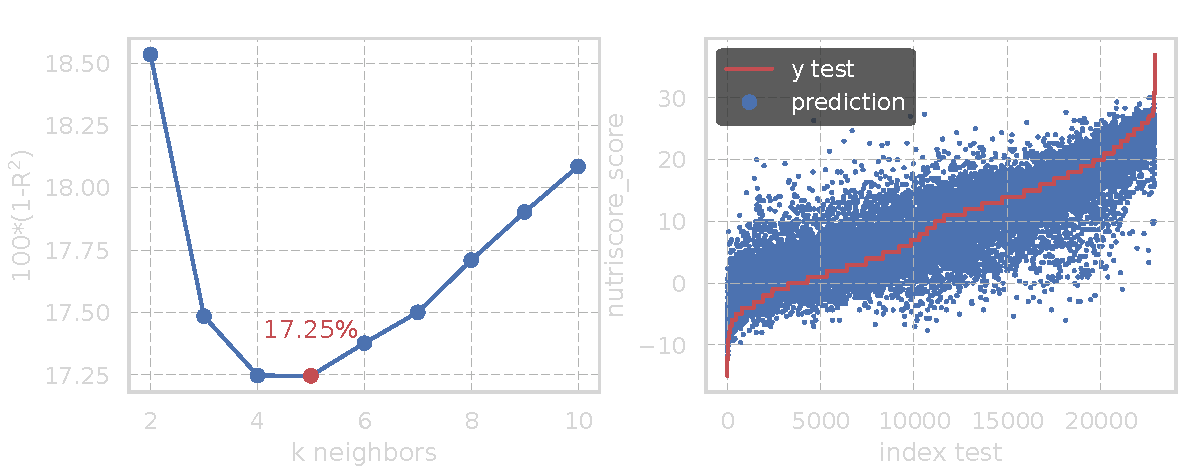
\includegraphics[width=90mm]{knn/1.pdf}
			} ;
		}
		\only<3->{
			\begin{scope}[yshift=-10mm]
				\node[anchor=west] at (0.2\textwidth,0.37\textheight) {$\rightarrow$ Amélioration \alert{non significative}} ;
				\node[anchor=west] at (0.2\textwidth,0.33\textheight) {$\rightarrow$ \alert{Centrage} et \alert{mise à l'échelle} des données} ;
			\end{scope}

		}

	\end{tikzpicture}
\end{frame}

\begin{frame}[t, label=knnUpgraded2]
	\vspace{0mm}
	\begin{tikzpicture}
		\linespread{1}% <--- locally defined vertical line spacing in nodes
		\draw[clrBorders] (0,0) rectangle (\textwidth,\textheight) ;

		\node[anchor=west] at (5mm,0.9\textheight) {Centrage et mise à l'échelle des données (par variable):} ;

		\visible<2->{
			\begin{scope}[yshift=0.8\textheight]
				\node[box_style0, text width=25mm] (A) at (0.3\textwidth,0) {Soustraction de la \alert{valeur moyenne}} ;

				\visible<3->{
					\node[box_style0, text width=25mm] (B) at (0.7\textwidth,0) { Normalisation de la \alert{variance} } ;
					\draw[myarrow] (A) -- (B) ;
				}
			\end{scope}
		}

		\only<4->{
			\node at (0.48\textwidth,0.5\textheight) {
				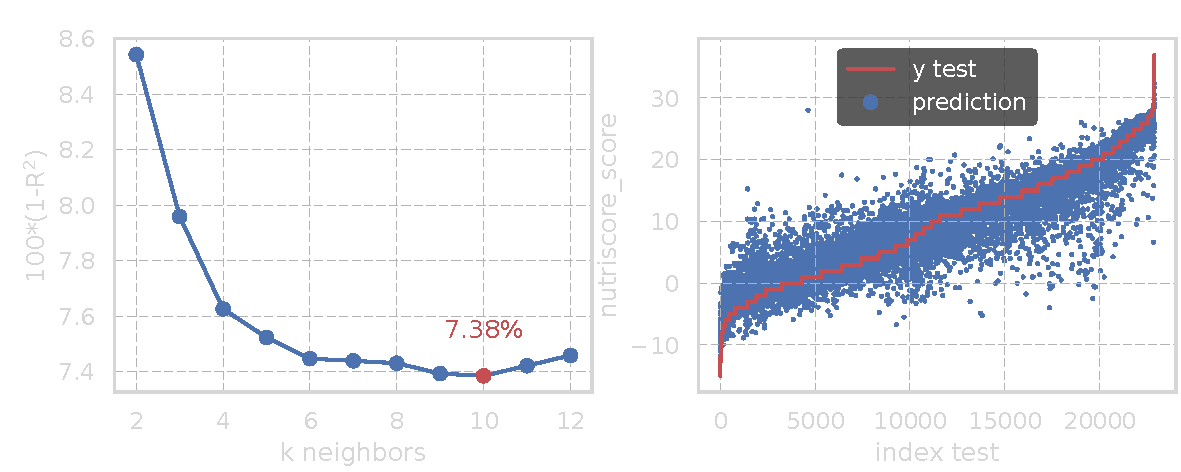
\includegraphics[width=90mm]{knn/2.pdf}
			} ;
		}
		\only<5->{
			\begin{scope}[yshift=-12mm]
				\node[anchor=west] at (0.2\textwidth,0.37\textheight) {$\rightarrow$ \alert{Nette} amélioration} ;
			\end{scope}
		}
		\visible<6->{
			\node[text centered] at (0.5\textwidth,10mm) {Quid de l'\alert{hypothèse} NaN fibers = 0 ? } ;
			}
	\end{tikzpicture}
\end{frame}


\begin{frame}[t, label=knnUpgraded3]
	\vspace{0mm}
	\begin{tikzpicture}
		\linespread{1}% <--- locally defined vertical line spacing in nodes
		\draw[clrBorders] (0,0) rectangle (\textwidth,\textheight) ;

		\node[anchor=west] at (5mm,0.9\textheight) {Vérification de l'hypothèse NaN fiber = 0:} ;

		\only<1->{
			\node at (0.48\textwidth,0.55\textheight) {
				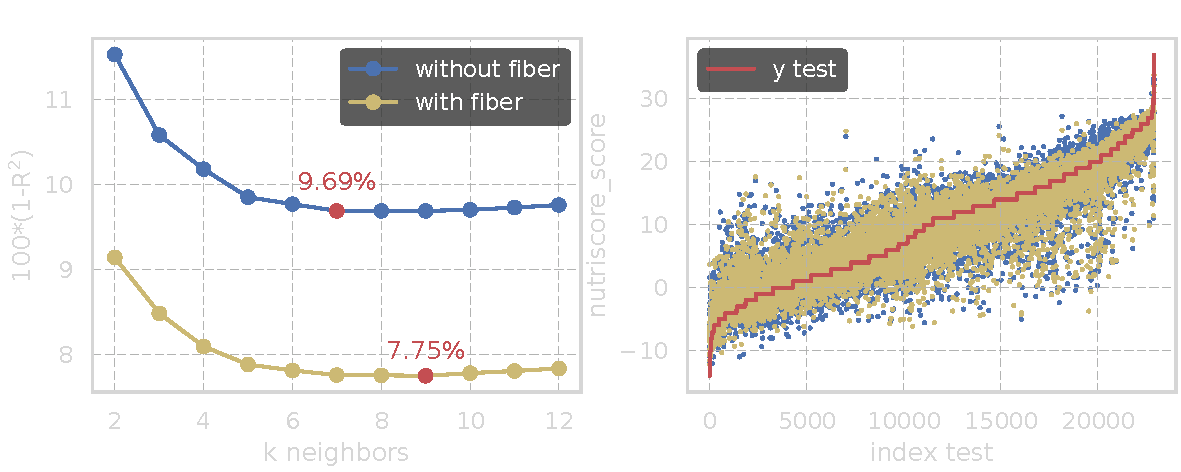
\includegraphics[width=90mm]{knn/3.pdf}
			} ;
		}
		\only<2->{
			\begin{scope}[yshift=-12mm]
				\node[anchor=west] at (0.2\textwidth,0.37\textheight) {$\rightarrow$ Hypothèse à priori \alert{validée} } ;
			\end{scope}
		}

	\end{tikzpicture}
\end{frame}


\section{PCA - projection}

\begin{frame}[t, label=pcaProjection]
	\vspace{0mm}
	\begin{tikzpicture}
		\linespread{1}% <--- locally defined vertical line spacing in nodes
		\draw[clrBorders] (0,0) rectangle (\textwidth,\textheight) ;

		\begin{scope}[xshift=0.5\textwidth, yshift=0.5\textheight]
			\visible<1>{
				\node at (0,0) {
					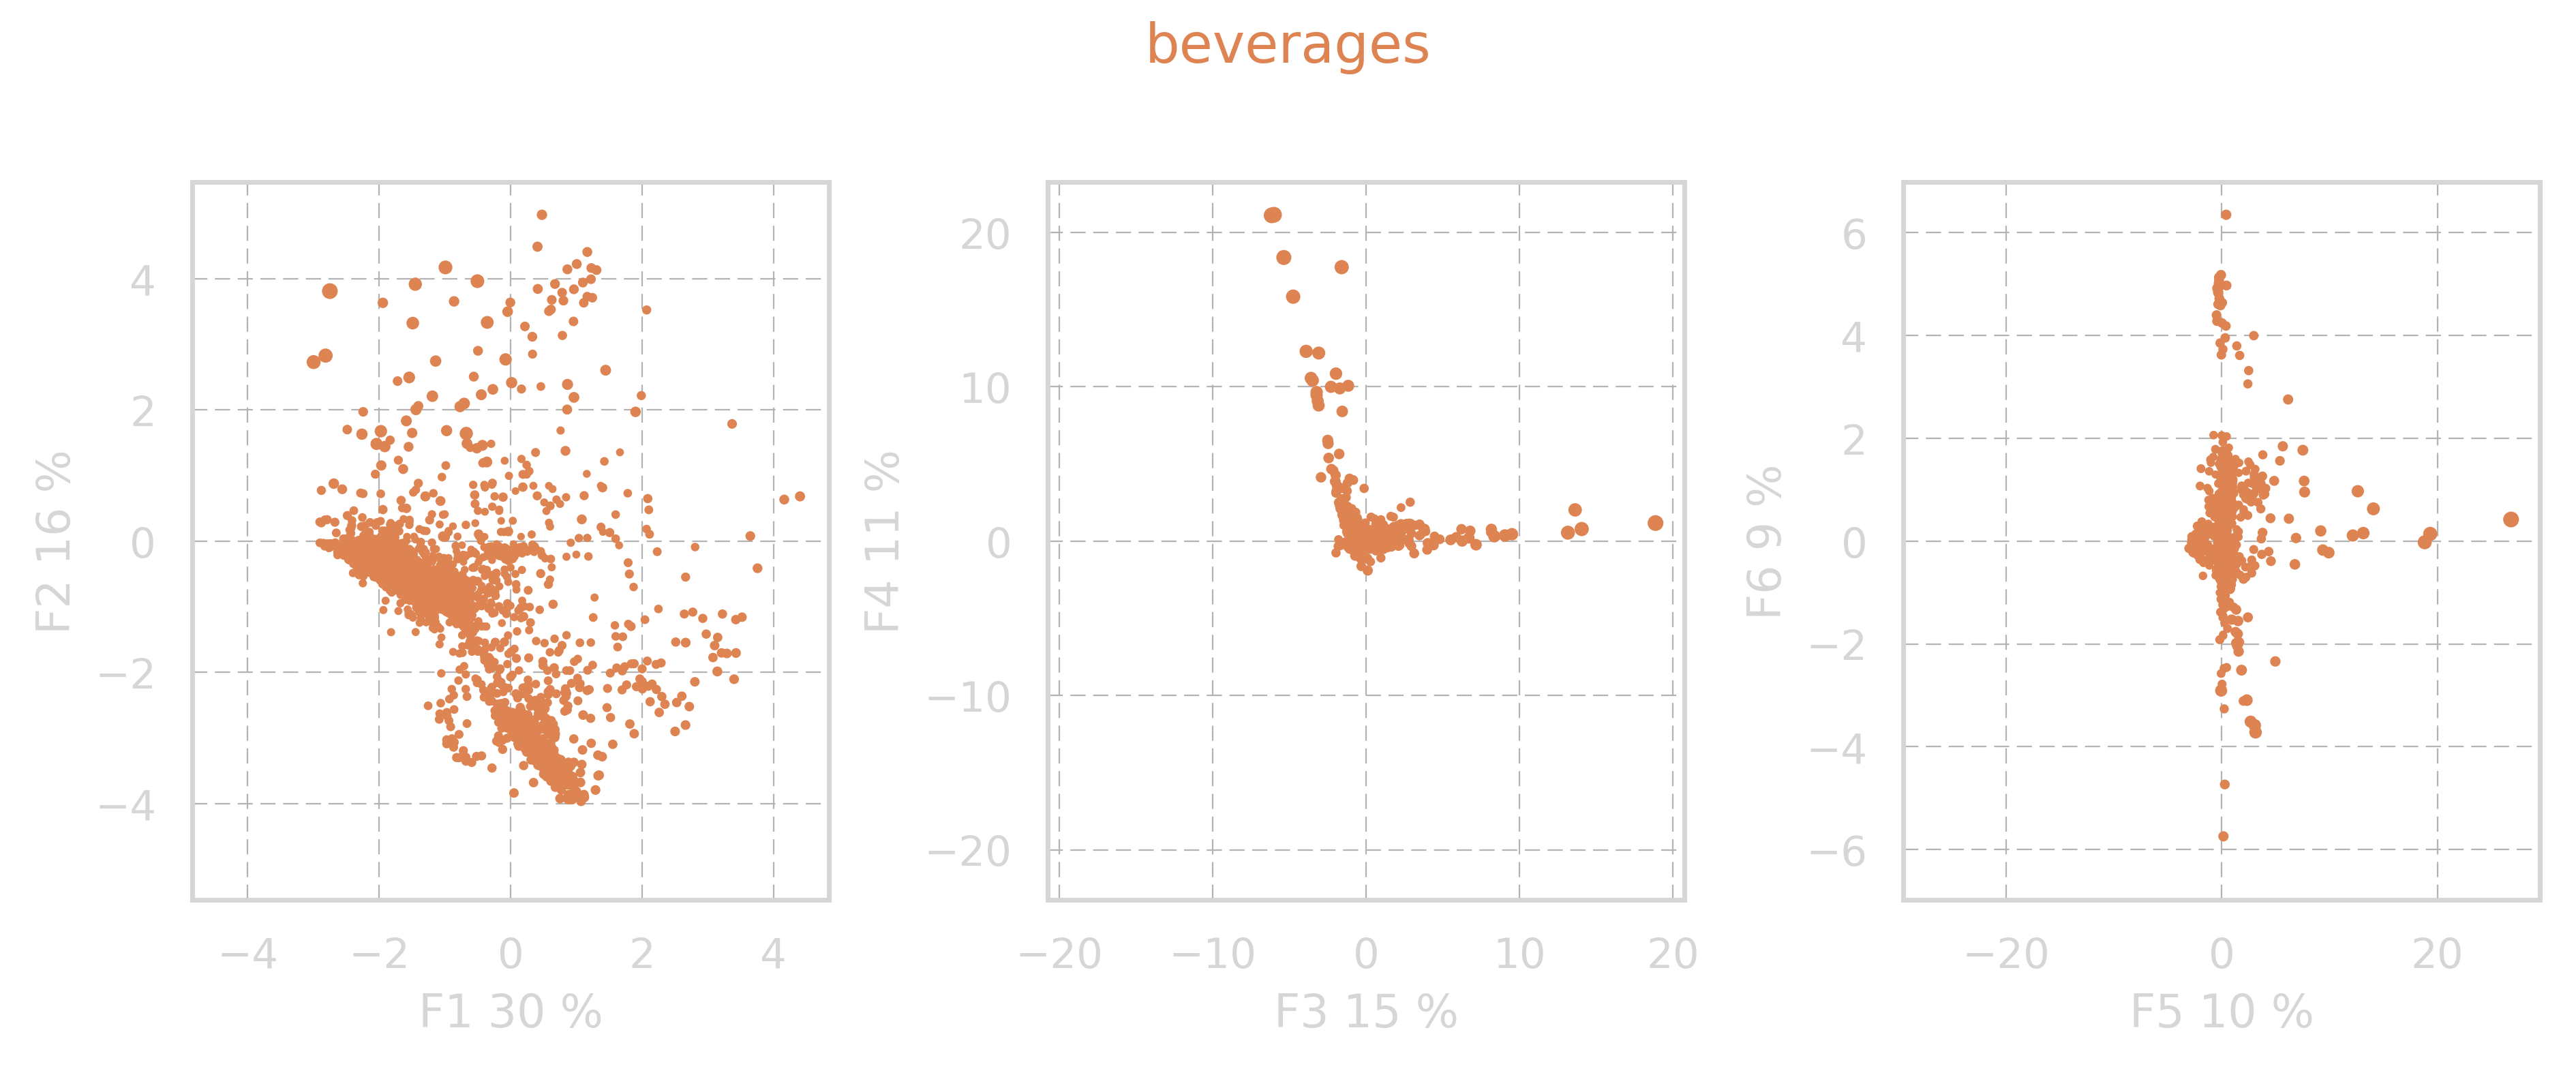
\includegraphics[width=100mm]{PCA/projection-beverages.png}
				} ;
			}

			\visible<2>{
				\node at (0,0) {
					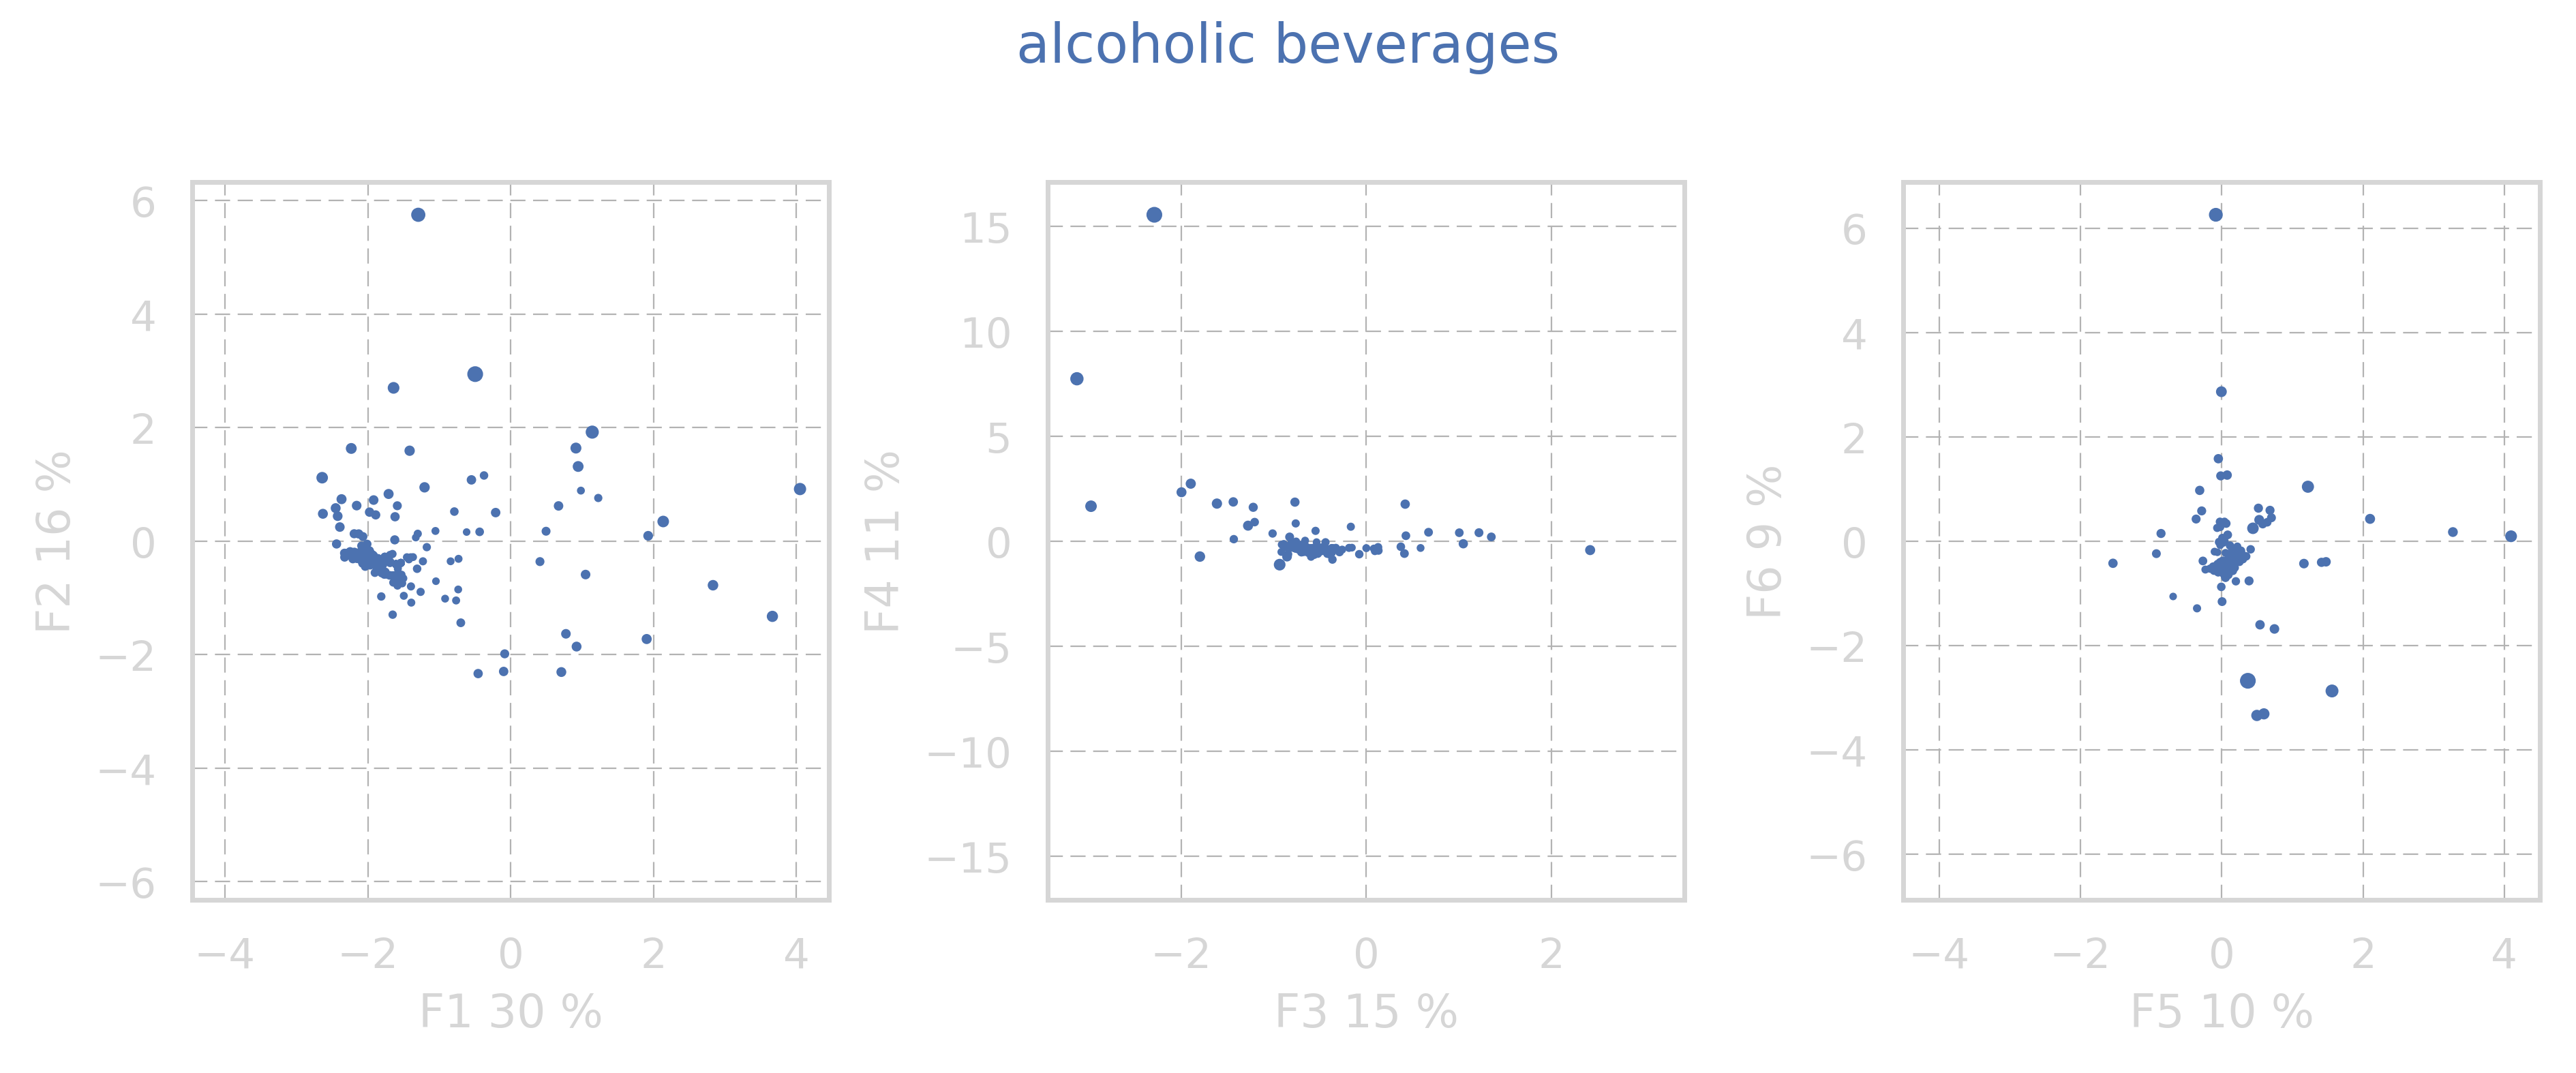
\includegraphics[width=100mm]{PCA/projection-alcoholic-beverages.png}
				} ;
			}

			\visible<3>{
				\node at (0,0) {
					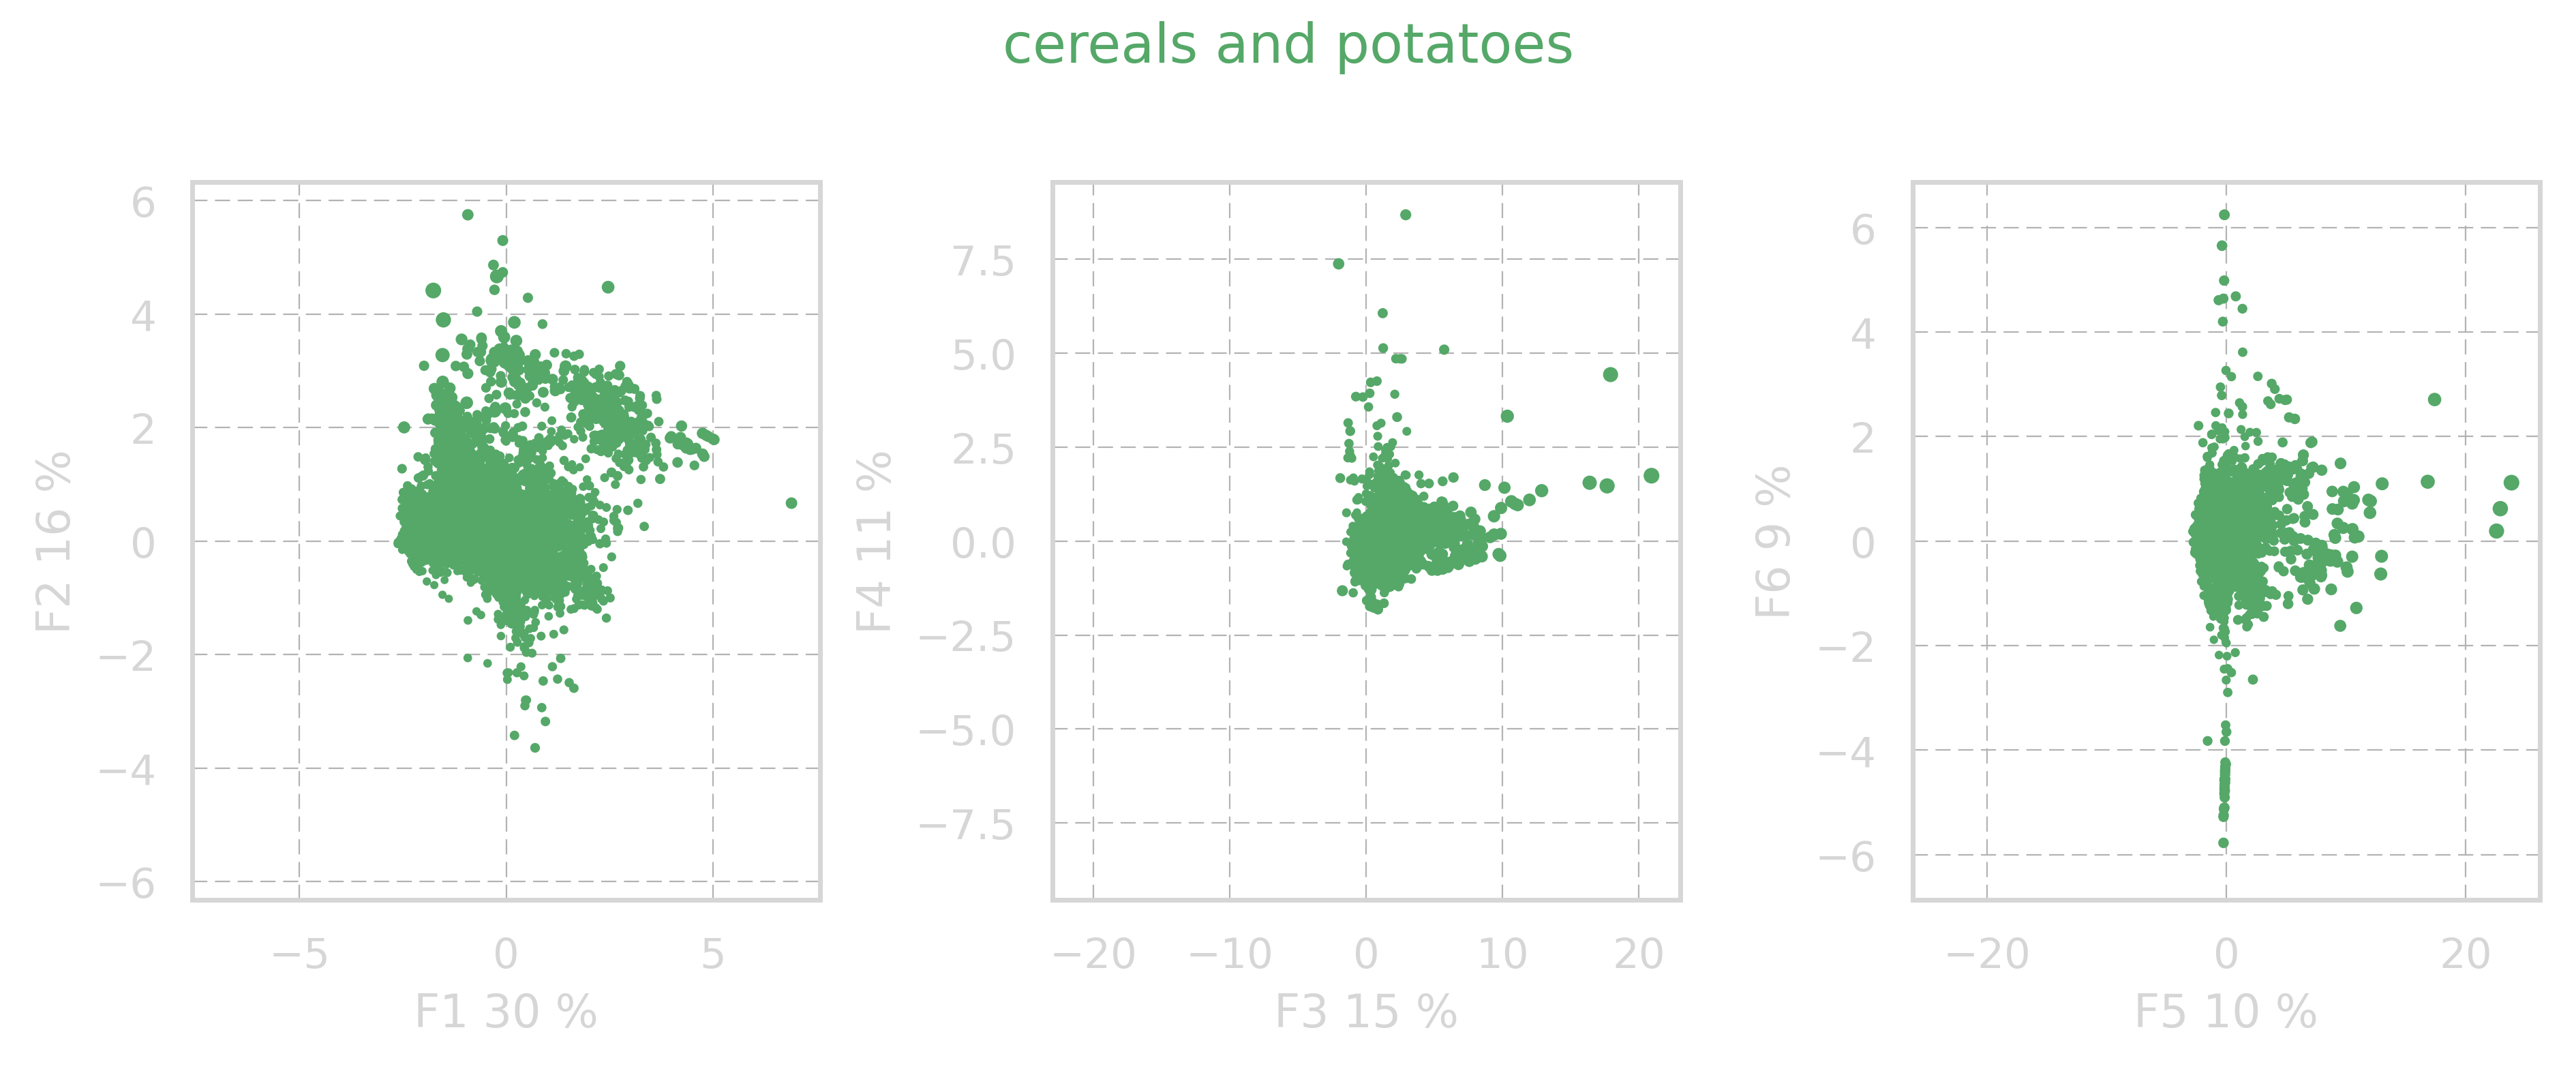
\includegraphics[width=100mm]{PCA/projection-cereals-and-potatoes.png}
				} ;
			}

			\visible<4>{
				\node at (0,0) {
					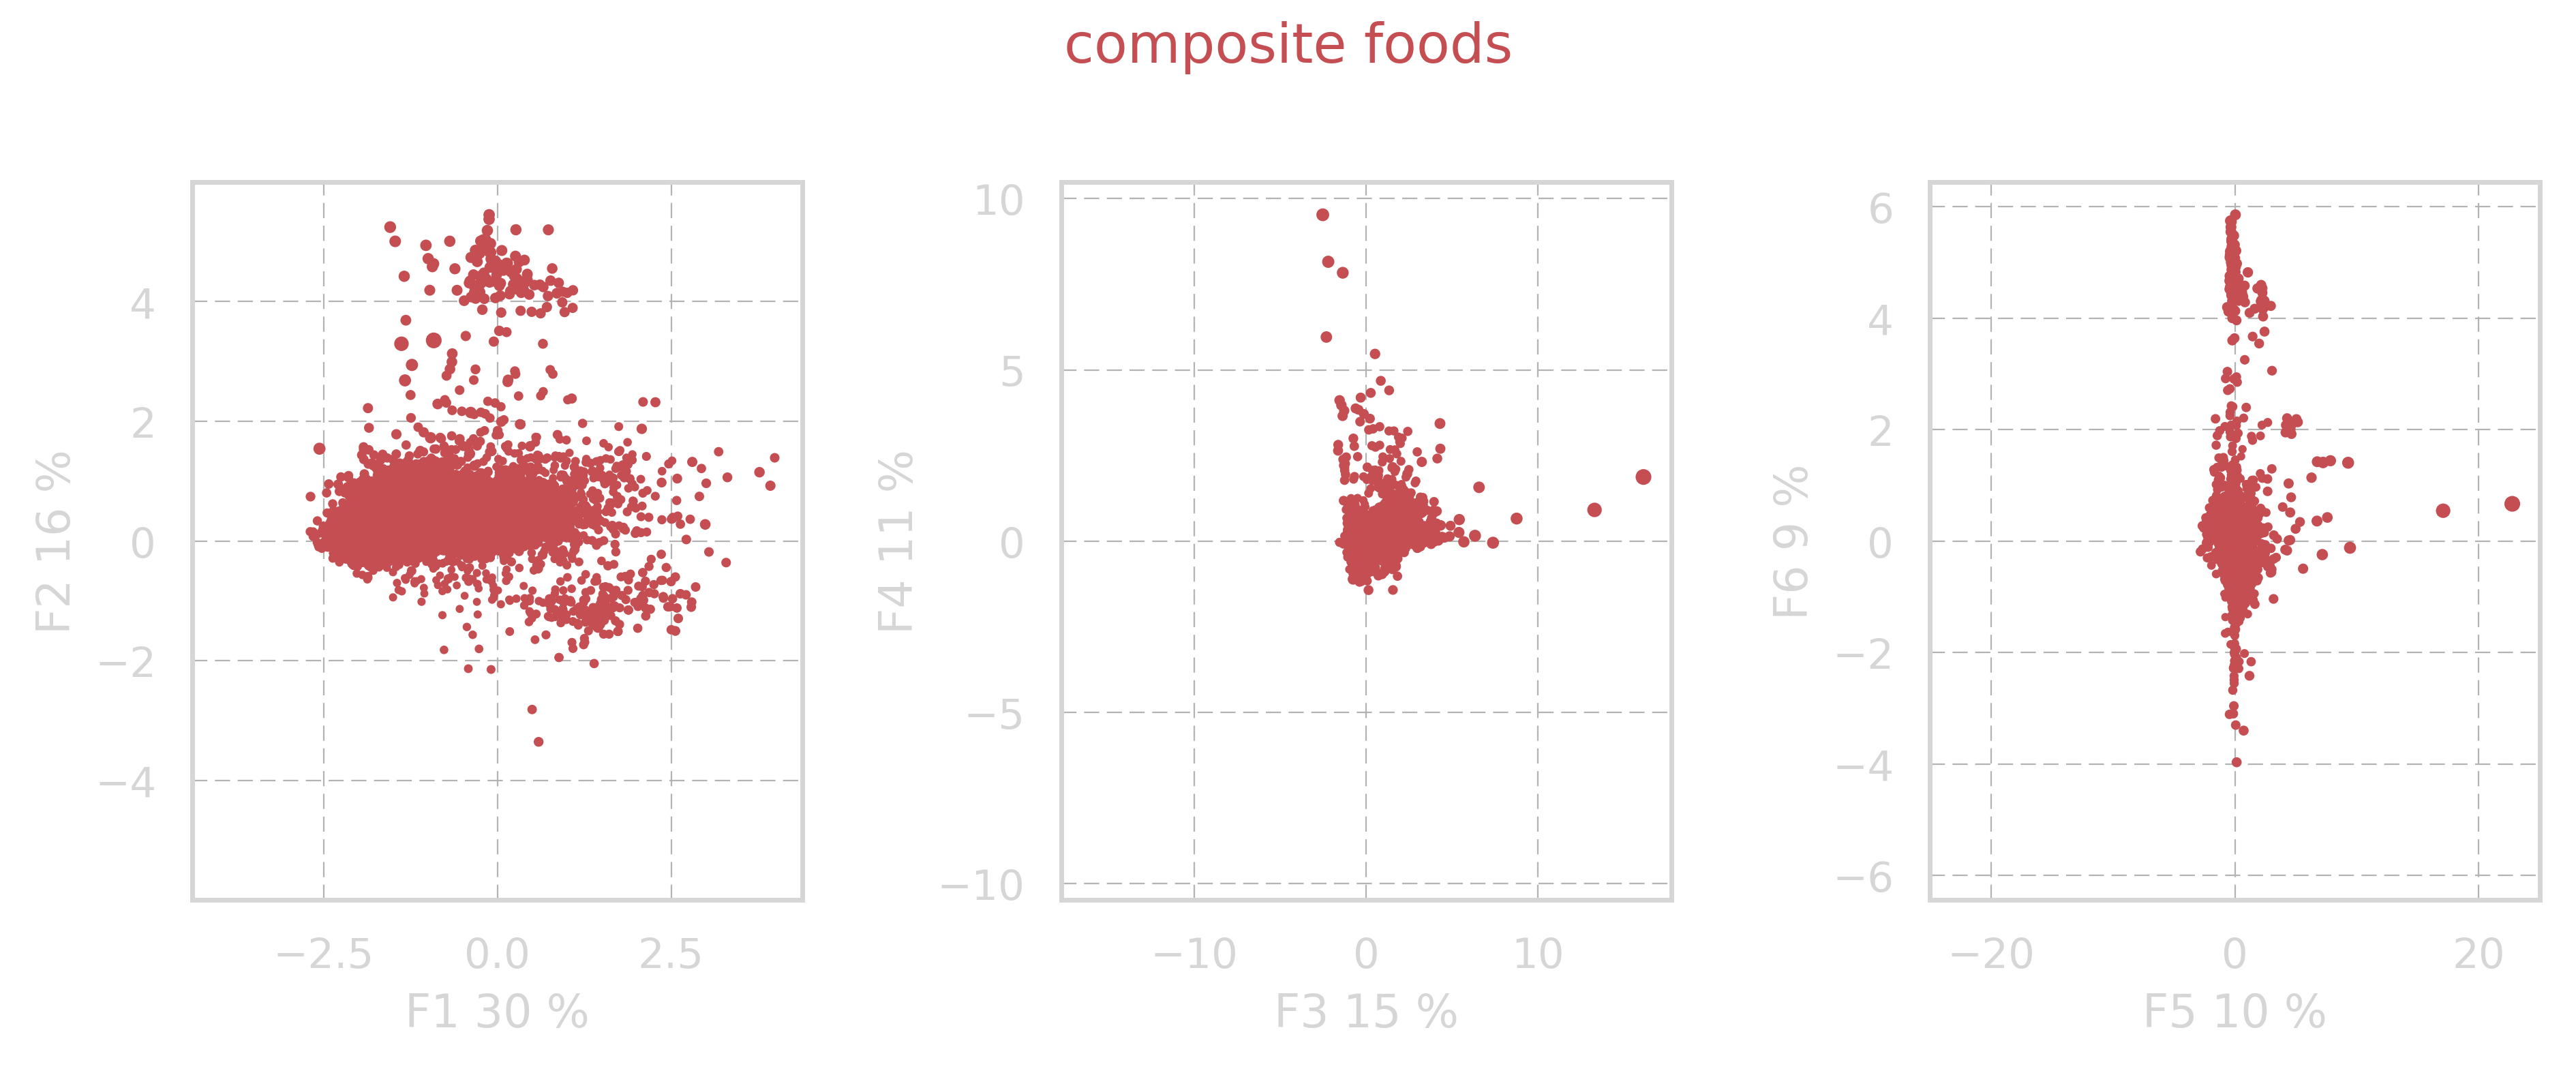
\includegraphics[width=100mm]{PCA/projection-composite-foods.png}
				} ;
			}

			\visible<5>{
				\node at (0,0) {
					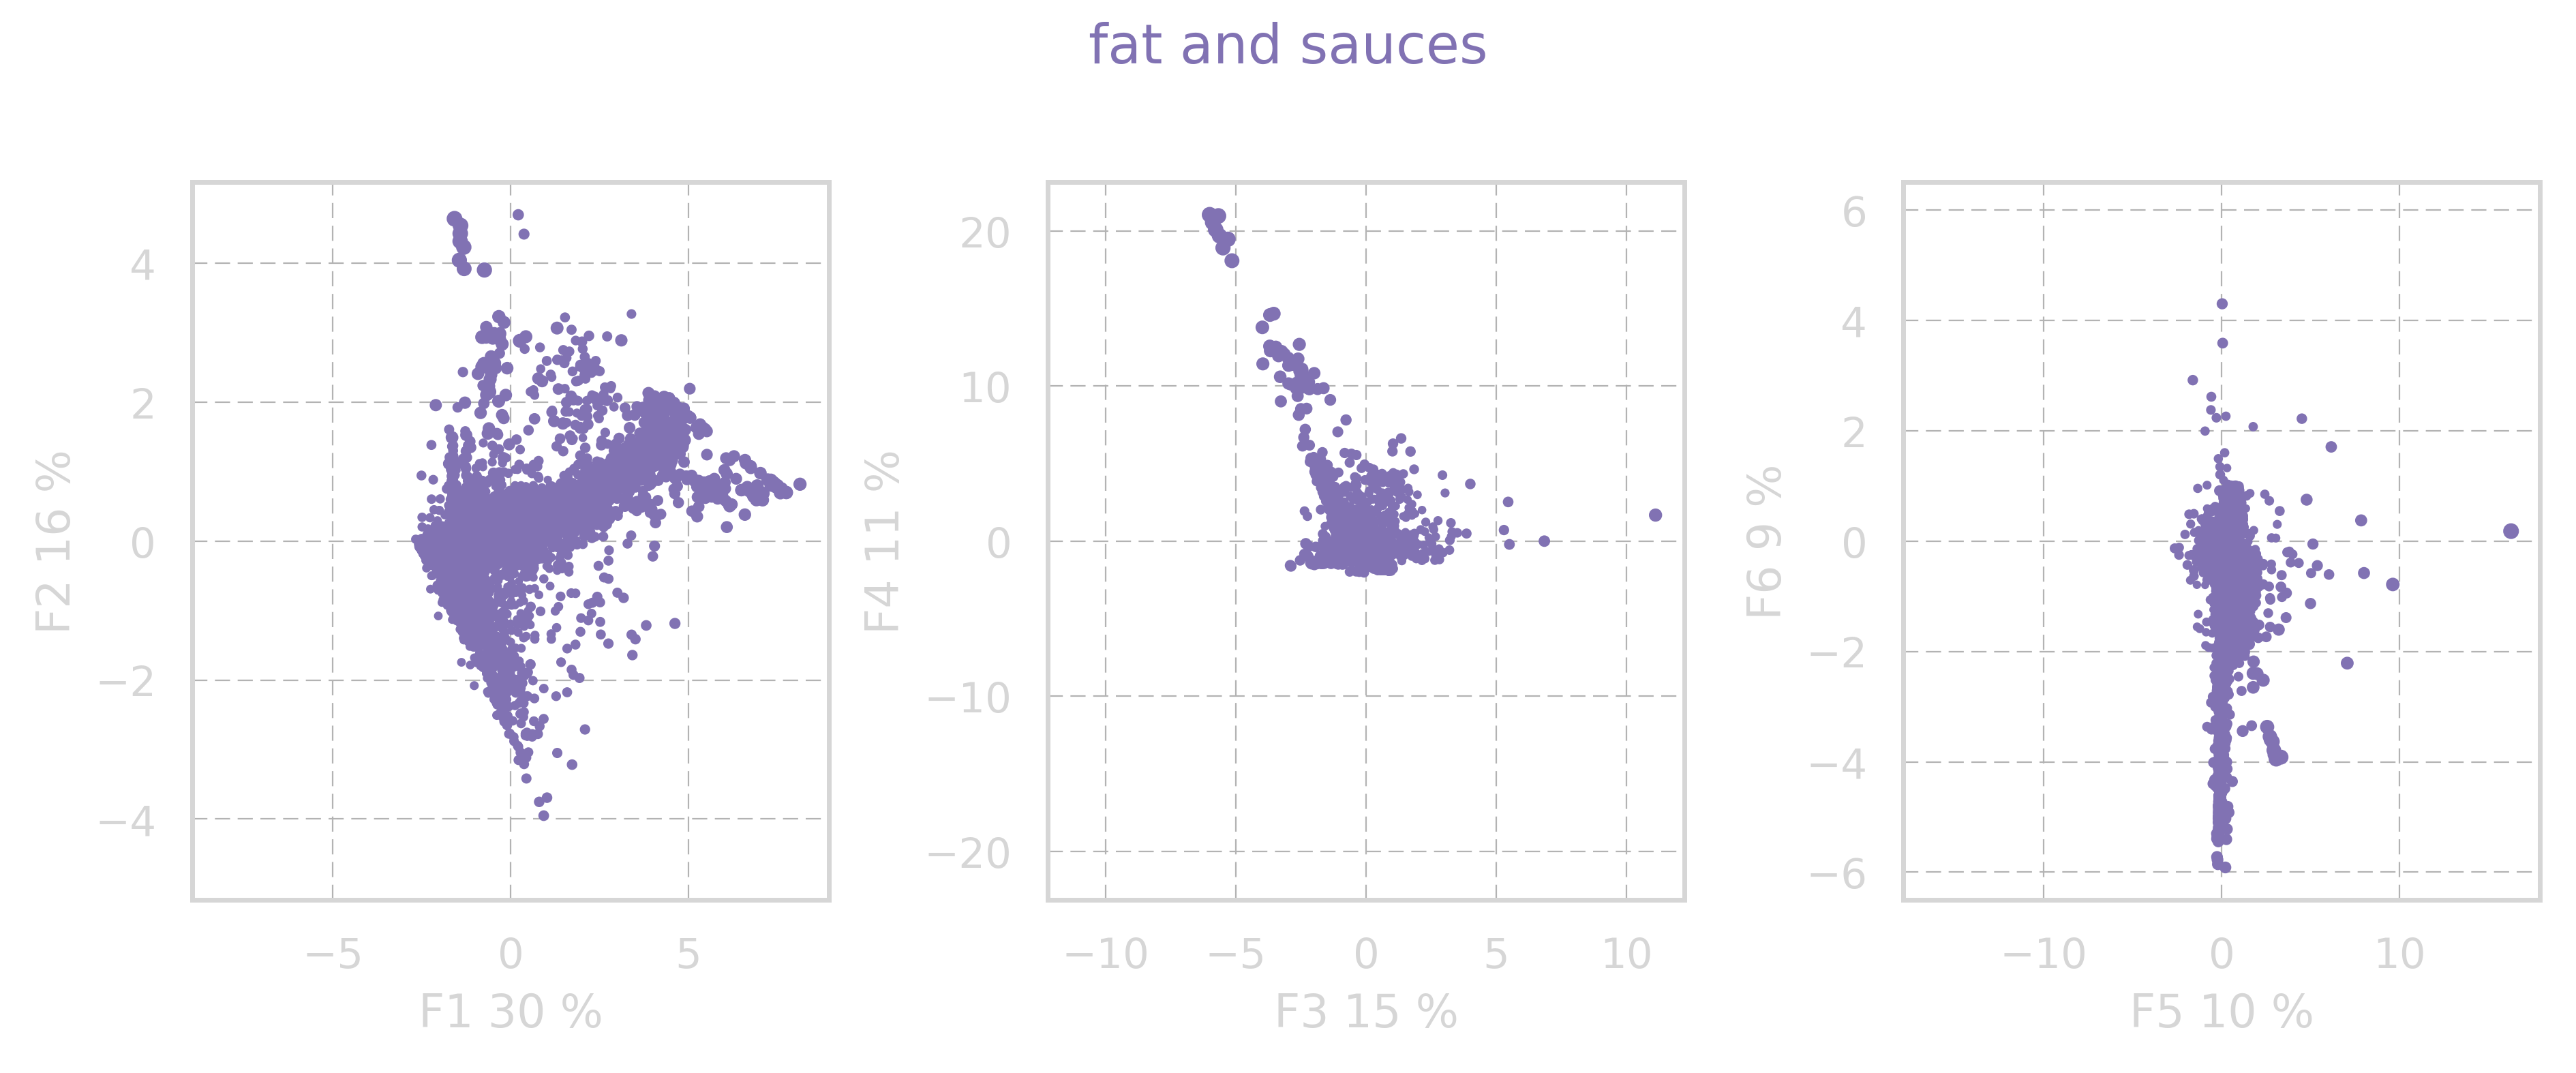
\includegraphics[width=100mm]{PCA/projection-fat-and-sauces.png}
				} ;
			}

			\visible<6>{
				\node at (0,0) {
					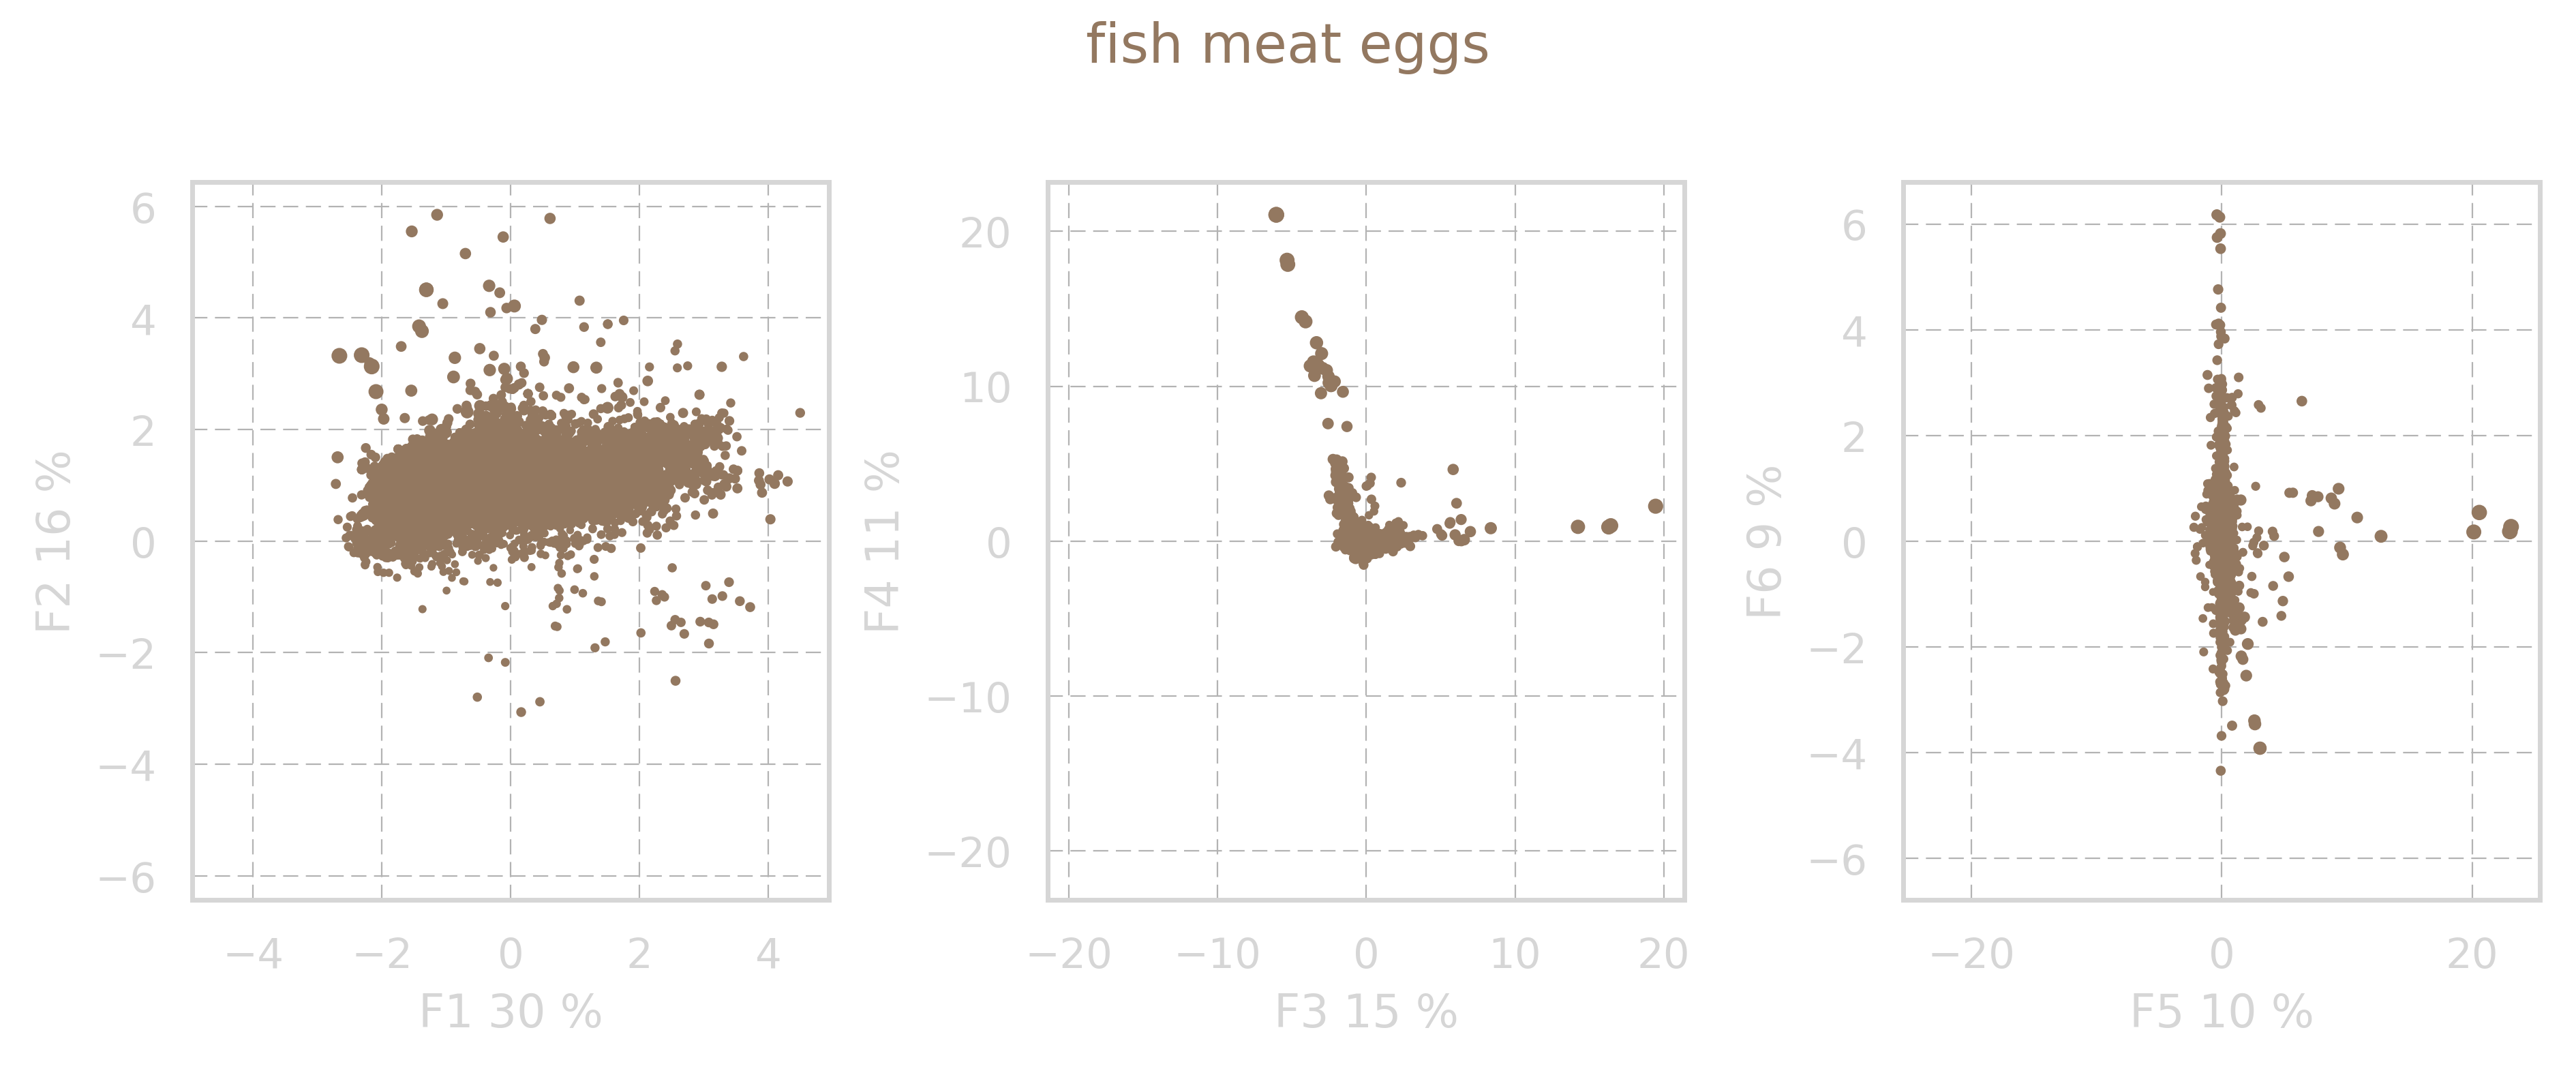
\includegraphics[width=100mm]{PCA/projection-fish-meat-eggs.png}
				} ;
			}

			\visible<7>{
				\node at (0,0) {
					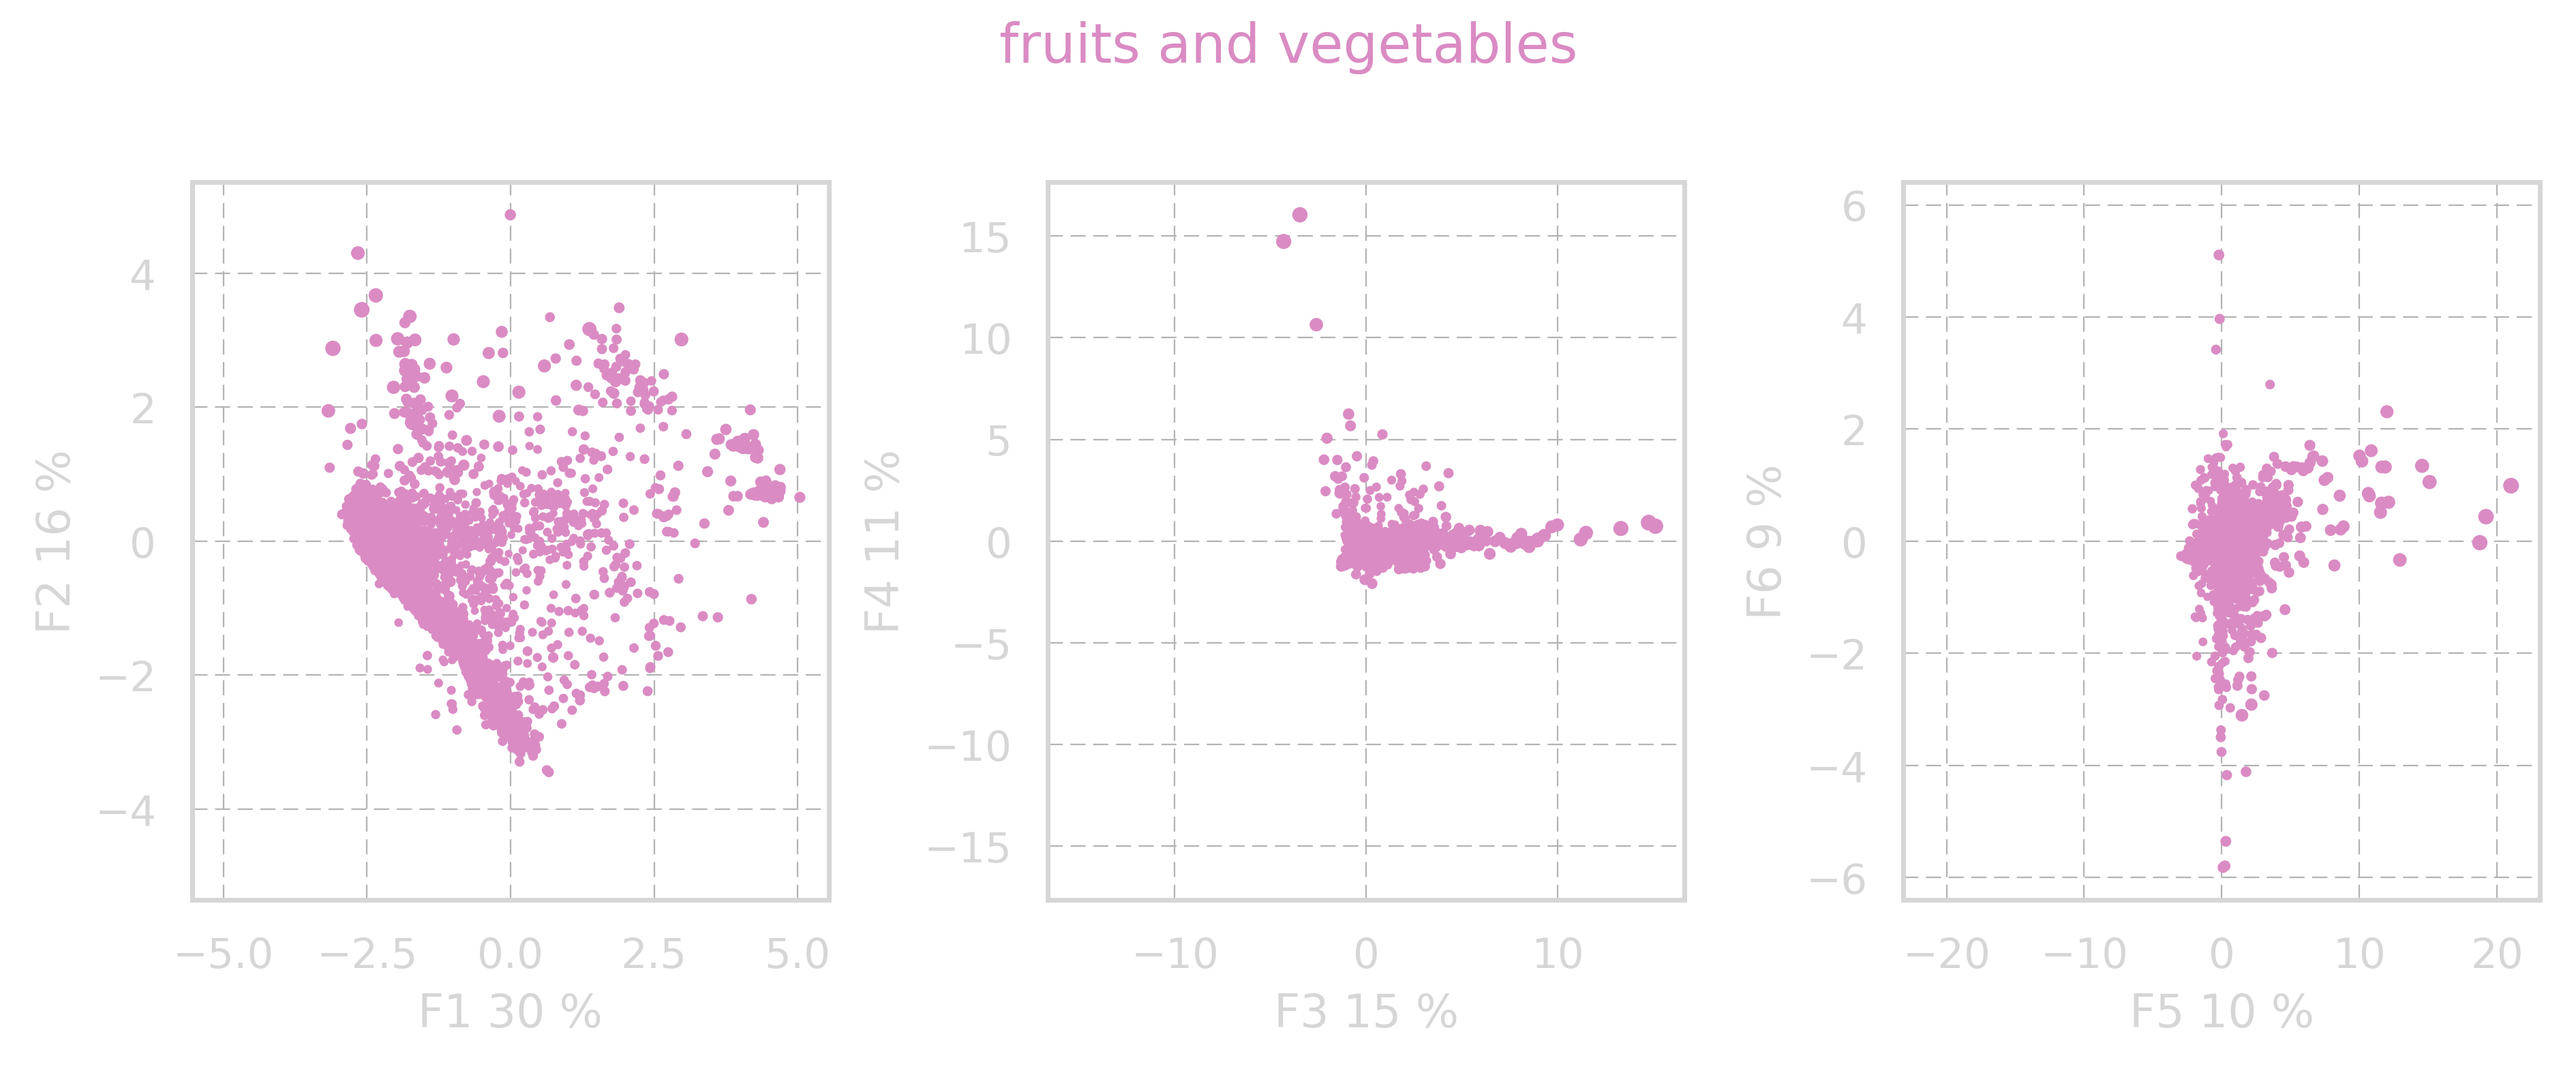
\includegraphics[width=100mm]{PCA/projection-fruits-and-vegetables.png}
				} ;
			}

			\visible<8>{
				\node at (0,0) {
					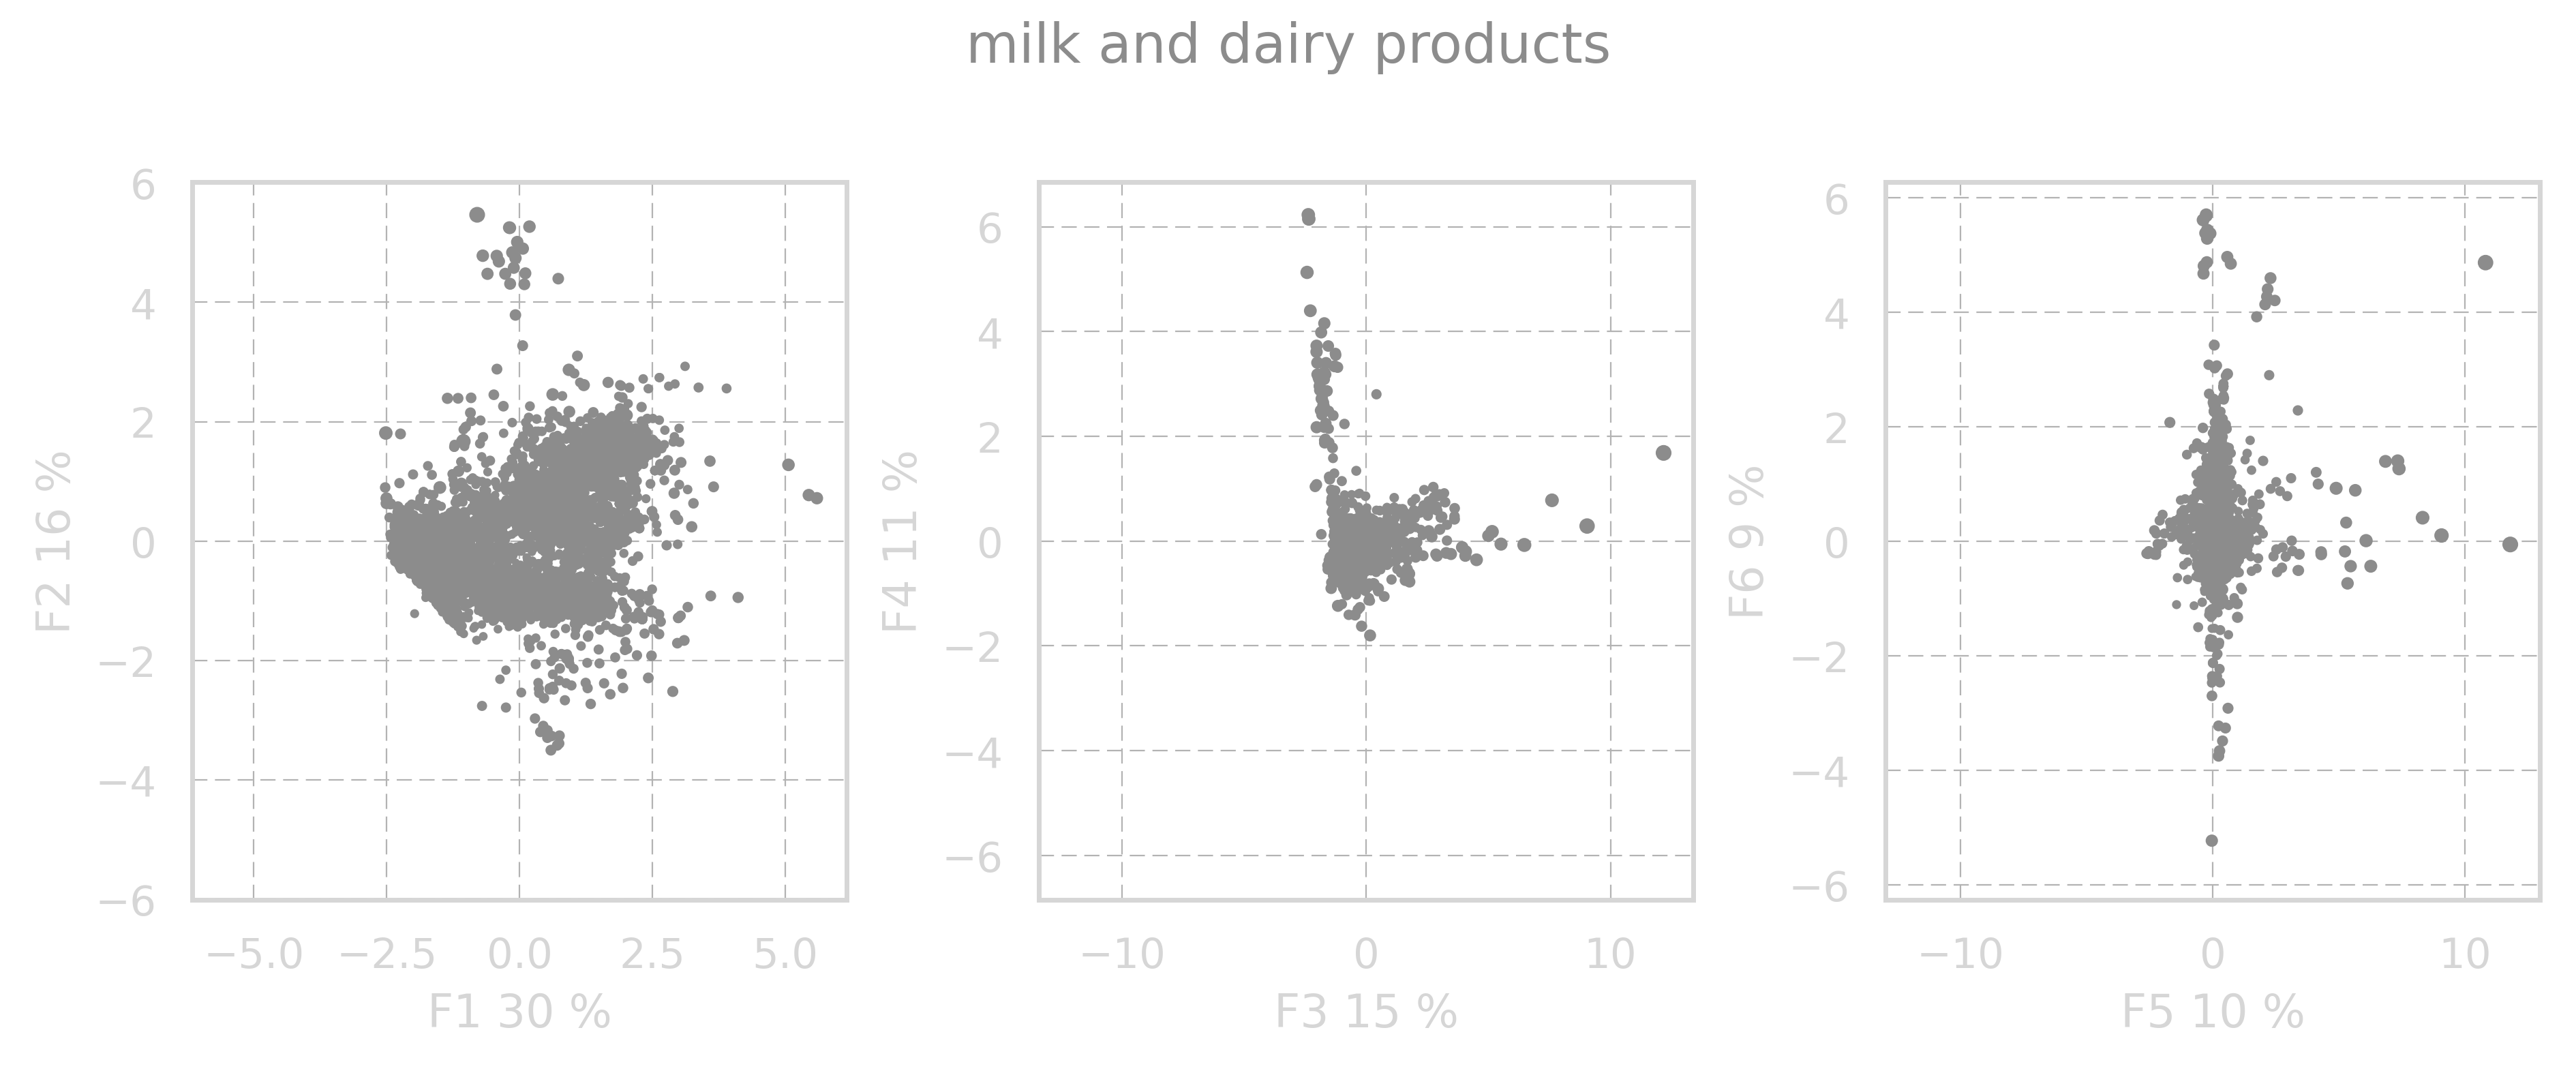
\includegraphics[width=100mm]{PCA/projection-milk-and-dairy-products.png}
				} ;
			}

			\visible<9>{
				\node at (0,0) {
					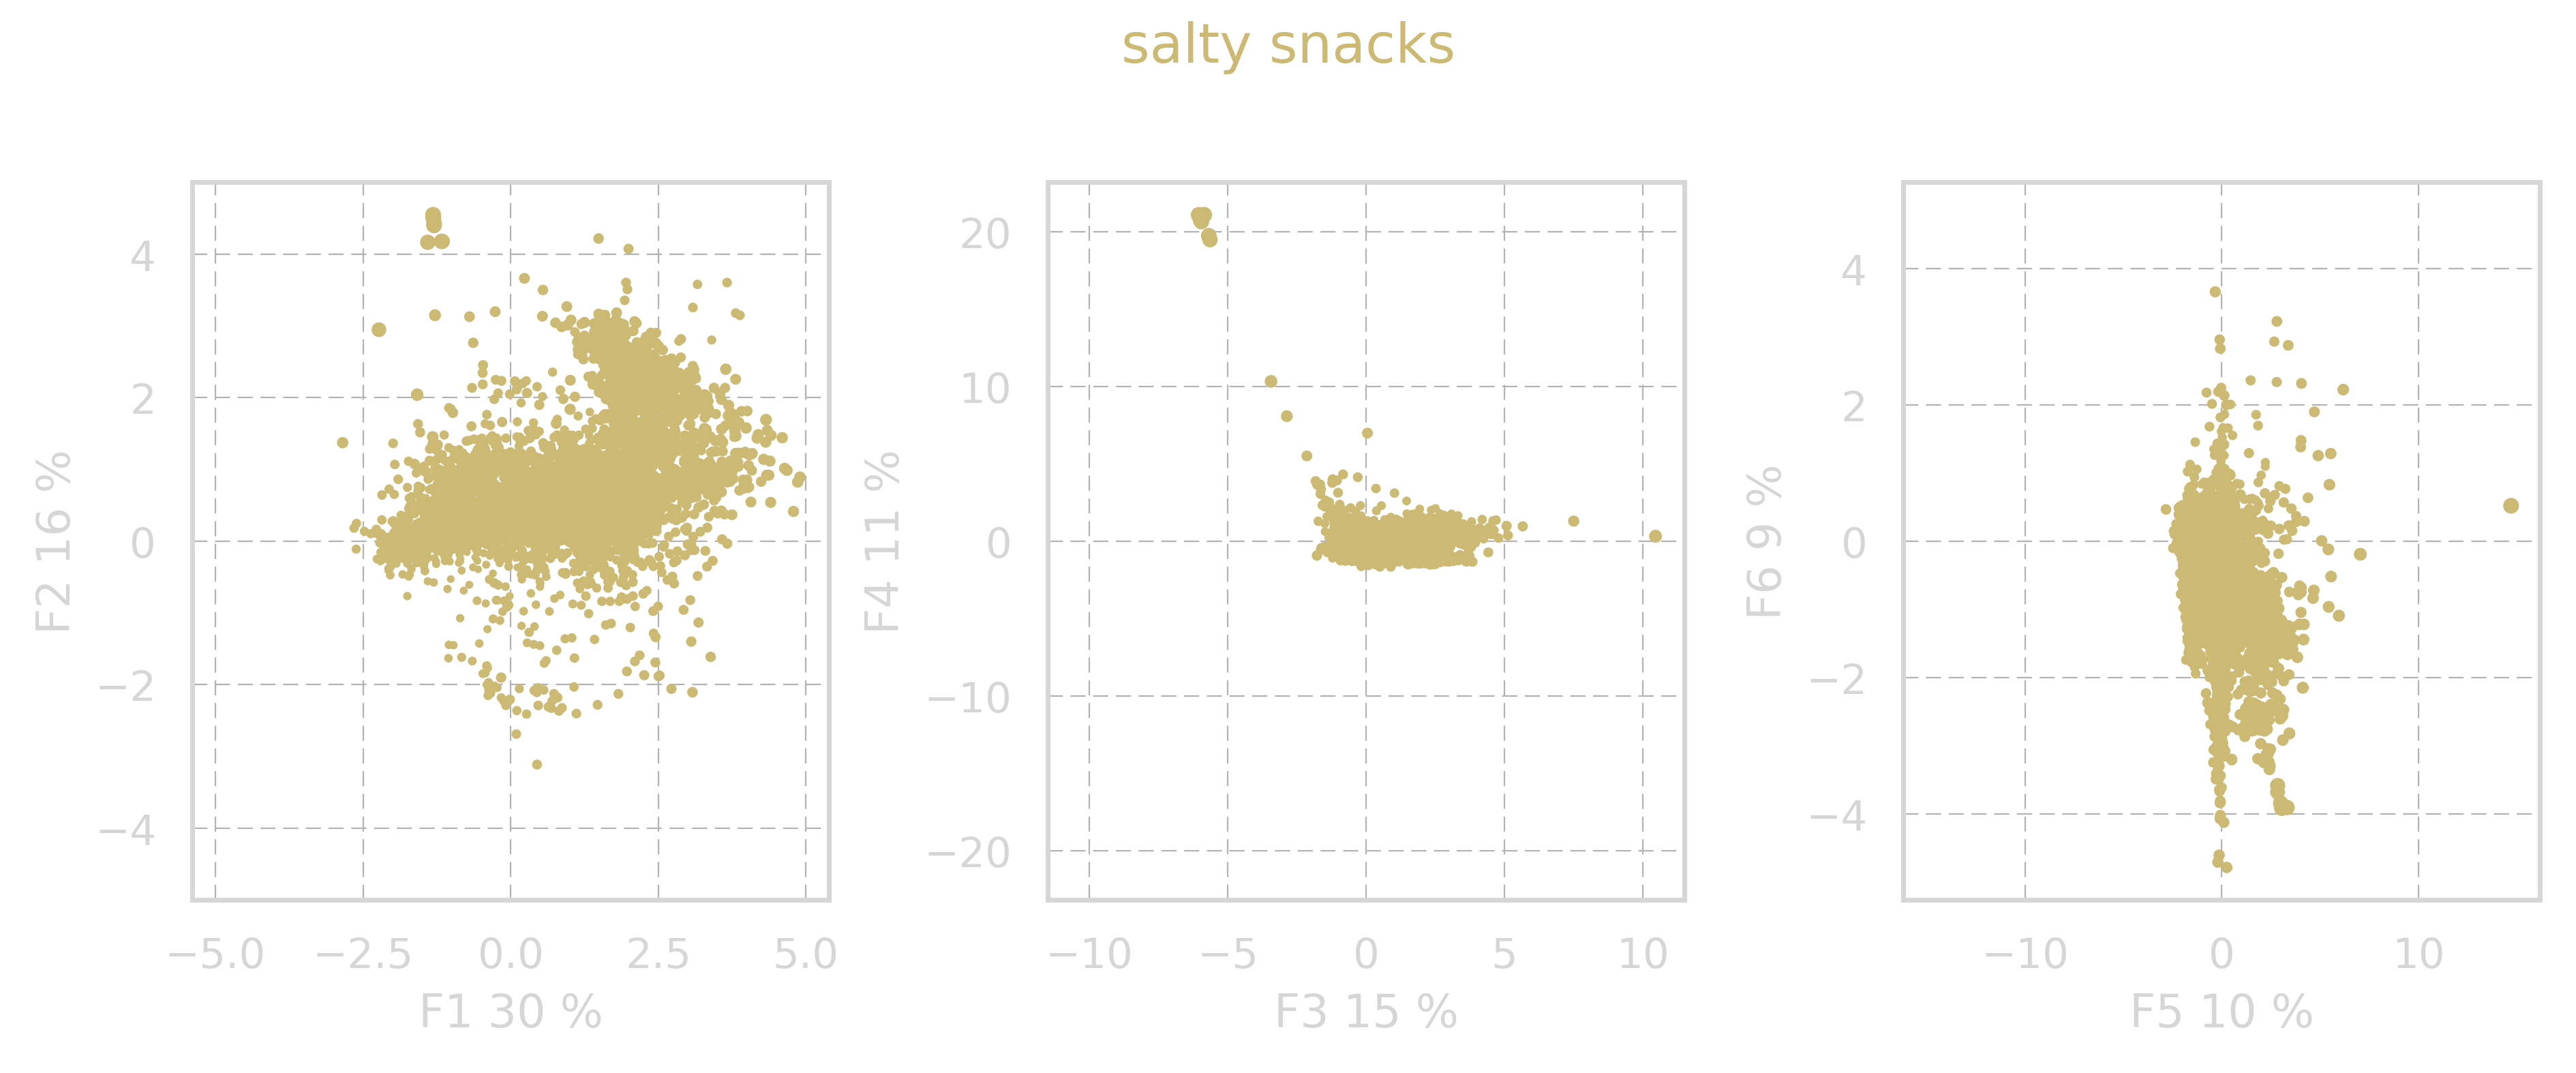
\includegraphics[width=100mm]{PCA/projection-salty-snacks.png}
				} ;
			}

			\visible<10>{
				\node at (0,0) {
					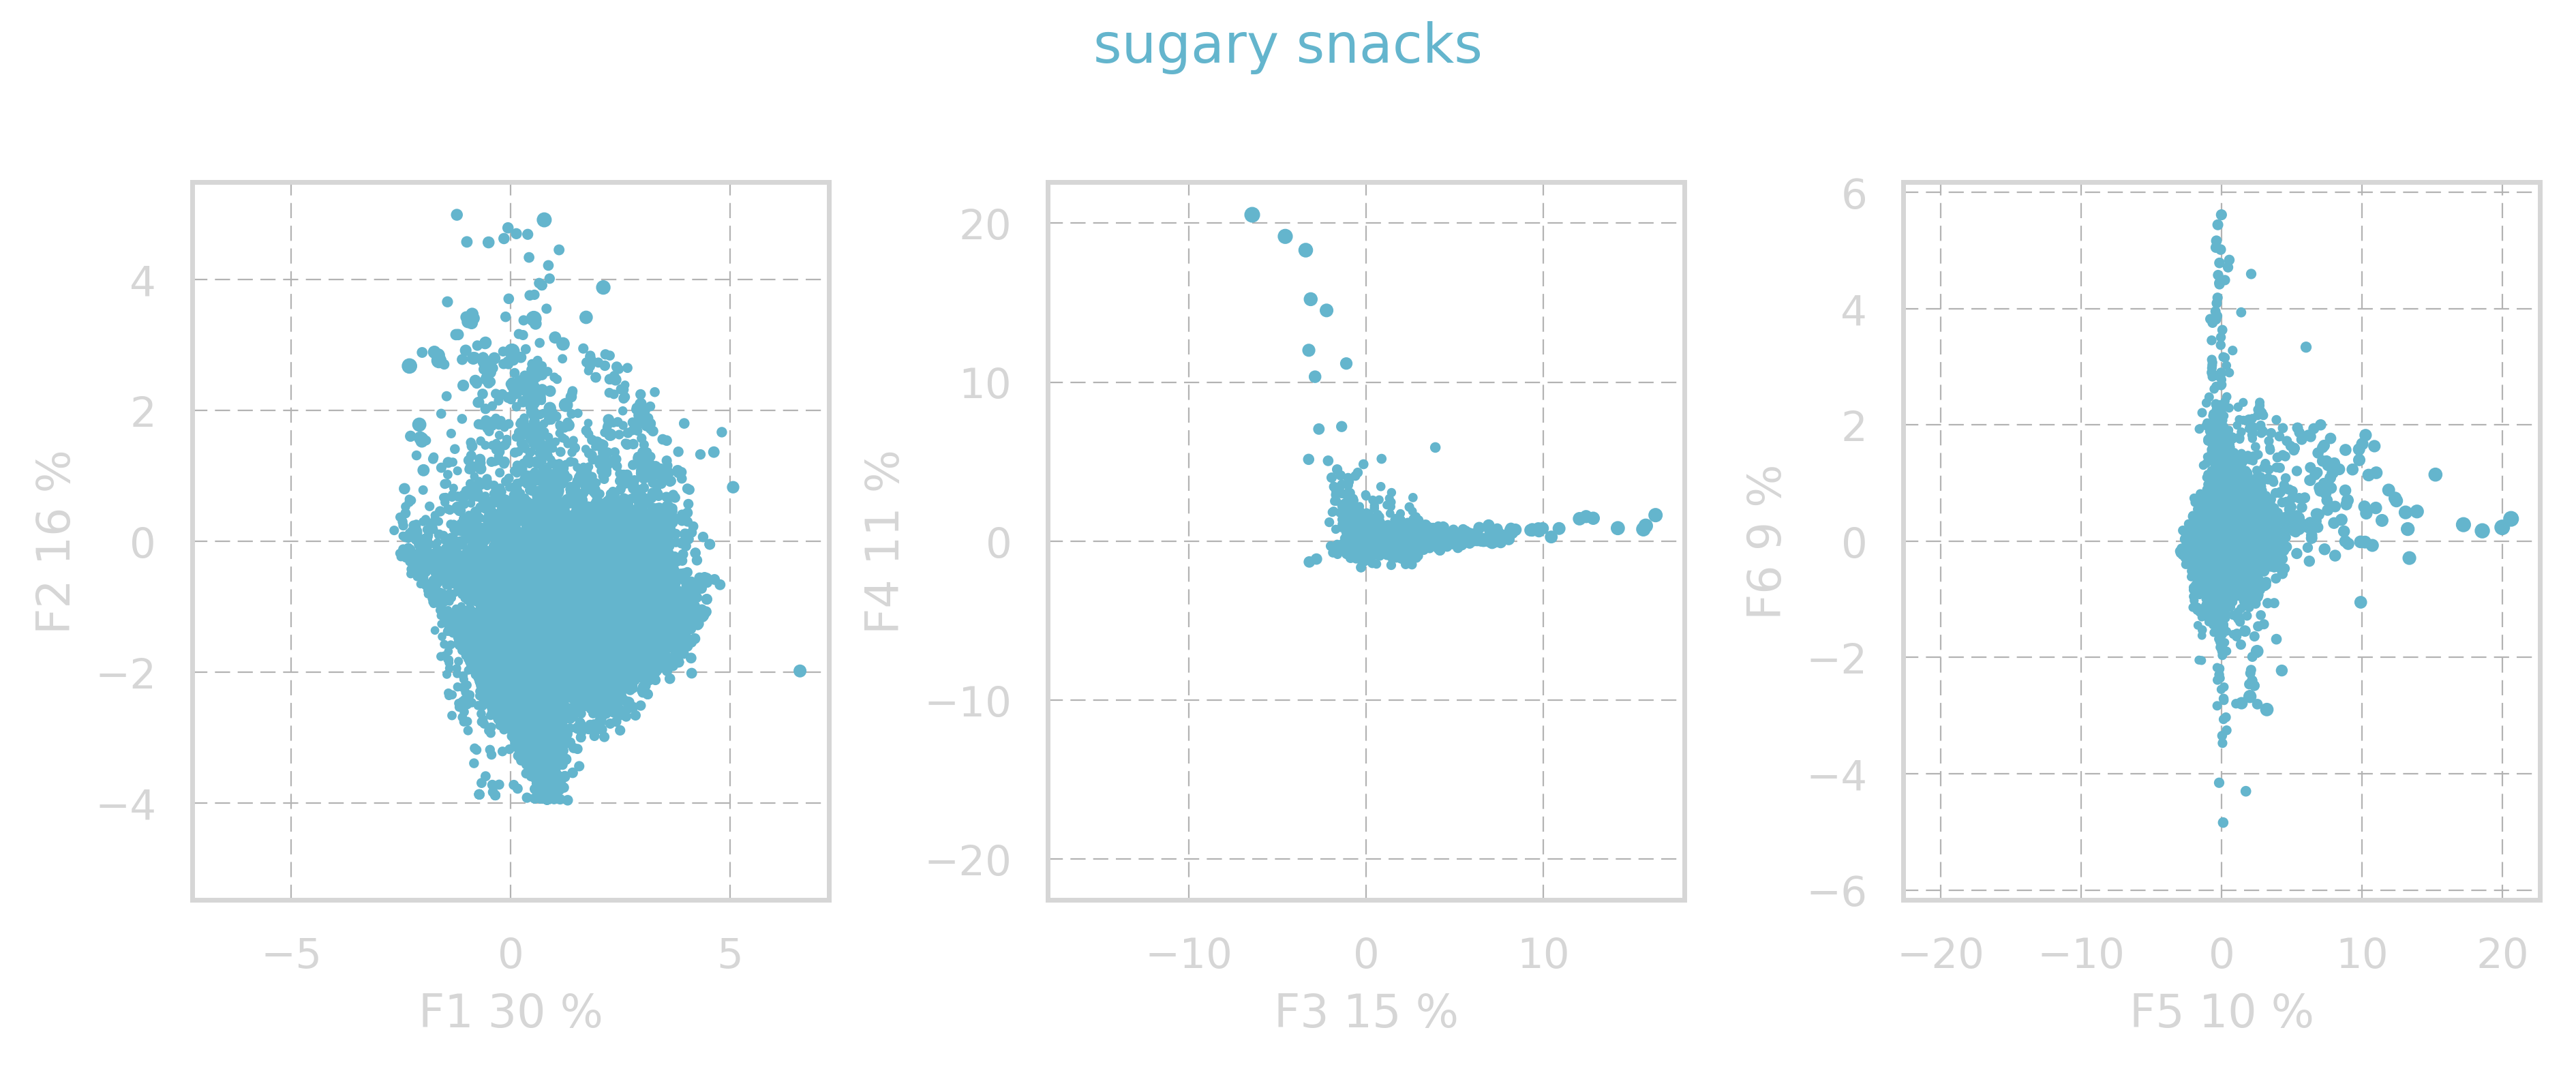
\includegraphics[width=100mm]{PCA/projection-sugary-snacks.png}
				} ;
			}
		\end{scope}

	\end{tikzpicture}
\end{frame}


\end{document}
